\chapter{Tensorflow进阶}
\section{模型存储和加载}
\begin{itemize}
\item 生成checkpoint文件,扩展名一般为.ckpt,通过在tf.train.Saver对象上调用Saver.saver()生成。它包含权重和其它程序中定义的变量,不包含
图的结构。如果需要在另一个程序中使用,需要重建图形结构,并告诉Tensorflow如何处理这些权重。
\item 生成(graph proto file),这是一个二进制文件,扩展名一般是.pb,用tf.train.write\_graph()保存,只包含图形结构,不包含权重,然后使用tf.import\_graph\_def()加载
图形。
\end{itemize}
\section{tf.estimator快速导航}
TensorFlow的高级机器学习API(tf.estimator)使得配置,训练评价多种机器学习模型变得很简单,在这个导航中,你将用tf.estimator构造一个神经网络分类器在\href{https://en.wikipedia.org/wiki/Iris_flower_data_set}{iris data}基于花萼和花瓣的几何特性训练预测花的种类,你的代码按照如下5步执行:
\begin{enumerate}
    \item 载入CSV文件的训练测试数据到TensorFlowDataset
    \item 构造\href{https://www.tensorflow.org/api_docs/python/tf/estimator/DNNClassifier}{神经网络分类器}
    \item 用训练数据训练模型。
    \item 评估模型的精度。
    \item 分类新的样本
\end{enumerate}
\subsection{完成神经网络源代码}
\lstinputlisting[language=Python]{./chapter2/code/iris_dnn_demo.py}
下面的章节将详细介绍代码。
\subsection{载入CSV数据进入TensorFlow}
\href{https://en.wikipedia.org/wiki/Iris_flower_data_set}{Iris data set}包含有150行iris样本:Iris setosa, Iris virginica和Iris versicolor。
\begin{figure}[H]
\includegraphics[width=\textwidth]{iris_three_species}
\end{figure}
每行的数据包括花萼的长宽,花瓣的长宽,花用整数代表0表示Iris setosa,1表示 Iris versicolor,2表示Iris virginica。
iris数据集已经被分成两部分
\begin{itemize}
    \item 120个样本的训练集\href{http://download.tensorflow.org/data/iris_training.csv}{iris\_training.csv}
    \item 30个样本的测试集\href{http://download.tensorflow.org/data/iris_test.csv}{iris\_test.csv}
\end{itemize}
导入需要的模型
\begin{lstlisting}[language=Python]
import os
import urllib.request

import numpy as np
import tensorflow as tf
#Ignore warning
os.environ['TF_CPP_MIN_LOG_LEVEL']='2' 

# Data sets
IRIS_TRAINING = "iris_training.csv"
IRIS_TRAINING_URL = "http://download.tensorflow.org/data/iris_training.csv"

IRIS_TEST = "iris_test.csv"
IRIS_TEST_URL = "http://download.tensorflow.org/data/iris_test.csv"
\end{lstlisting}
如果训练集和测试集没有被存储在本地,下载它们:
\begin{lstlisting}[language=Python]
if not os.path.exists(IRIS_TRAINING):
    raw = urllib.request.urlopen(IRIS_TRAINING_URL).read().decode('utf-8')
    with open(IRIS_TRAINING, "wb") as f:
      f.write(raw)

  if not os.path.exists(IRIS_TEST):
    raw = urllib.request.urlopen(IRIS_TEST_URL).read().decode('utf-8')
    with open(IRIS_TEST, "wb") as f:
      f.write(raw)
\end{lstlisting}
下一步用learn.dataset.base中的load\_csv\_with\_header()方法载入训练数据进入Dataset,load\_csv\_with\_header()方法接受三个参数:
\begin{itemize}
    \item filename:CSV文件的完成的路径加上文件名。
    \item target\_dtype:接收numpy datatype的数据集的目标值。
    \item feature\_dtype:接收numpy datatype类型的数据集的特征值。
\end{itemize}
这里的目标(你的训练模型的预测)是花的种类,值范围为0~2,因此合适的numpy数据类型是np.int。
\begin{lstlisting}[language=Python]
# Load datasets.
training_set = tf.contrib.learn.datasets.base.load_csv_with_header(
    filename=IRIS_TRAINING,
    target_dtype=np.int,
    features_dtype=np.float32)
test_set = tf.contrib.learn.datasets.base.load_csv_with_header(
    filename=IRIS_TEST,
    target_dtype=np.int,
    features_dtype=np.float32)
\end{lstlisting}
在tf.contrib.learn中的Dataset是\href{https://docs.python.org/2/library/collections.html#collections.namedtuple}{named tuples};你可以通过data和target访问特征数据和目标值,这里training\_set.data和training\_set.target包含训练集的特征数据和目标数据,对应的test\_set.data和test\_set.target包含测试集特征和目标。
\subsection{构造神经网络分类器}
tf.estimator提供多种预定义方法,称为Estimator,你可以通过它在你的数据上运行训练,评估操作,你可以实例化tf.estimator.DNNClassfier:
\begin{lstlisting}[language=Python]
# Specify that all features have real-value data
feature_columns = [tf.feature_column.numeric_column("x", shape=[4])]

# Build 3 layer DNN with 10, 20, 10 units respectively.
classifier = tf.estimator.DNNClassifier(feature_columns=feature_columns,
                                        hidden_units=[10, 20, 10],
                                        n_classes=3,
                                        model_dir="./iris_model")
\end{lstlisting}
上面的代码中首先定义模型的特征列,指定在数据集中的特征的数据类型。所有的特征数据是连续的,因此tf.feature\_column.number\_column是构造特征列的合适的函数,数据集中有4个特征,因此我们指定shape为[4]保持所有的数据,然后用下面的参数创建DNNClassfier分类器模型:
\begin{itemize}
    \item feature\_columns=feature\_columns,特征集合的列。
    \item hidden\_units=[10,20,10],三个\href{http://stats.stackexchange.com/questions/181/how-to-choose-the-number-of-hidden-layers-and-nodes-in-a-feedforward-neural-netw}{hidden layer}包含有10,20,10个神经元。
    \item n\_classes=3,三个目标类,对应三个iris种类。
    \item model\_dir=./iris\_model:训练模型中保存checkpoint文件的路径
\end{itemize}
\subsection{描述训练的输入pipline}
tf.estimator API用输入函数创建TensorFlow操作为模型生成数据,你可以用\newline
tf.estimator.numpy\_input\_fn生成输入pipeline:
\begin{lstlisting}[language=Python]
# Define the training inputs
train_input_fn = tf.estimator.inputs.numpy_input_fn(
    x={"x": np.array(training_set.data)},
    y=np.array(training_set.target),
    num_epochs=None,
    shuffle=True)
\end{lstlisting}
\subsection{为iris训练集拟合DNNClassfier}
现在我们已经配置好的classfier模型,你可以用train方法通过训练数据训练模型。传递train\_input\_fn作为input\_fn,这里训练步数为2000:
\begin{lstlisting}[language=Python]
# Train model.
classifier.train(input_fn=train_input_fn, steps=2000)
\end{lstlisting}
状态模型被保存在classfier,意味着你可以反复训练,例如下面是合适的:
\begin{lstlisting}[language=Python]
classifier.train(input_fn=train_input_fn, steps=1000)
classifier.train(input_fn=train_input_fn, steps=1000)
\end{lstlisting}
然而,如果你在训练的时候跟踪模型,你可以用TensorFlow \href{https://www.tensorflow.org/api_docs/python/tf/train/SessionRunHook}{SessionRunHook}执行采集操作.
\subsection{评估模型的精度}
你可以在iris训练集上训练你的DNNClassfier模型;现在你可以在测试集上用evaluate检查它在测试集上个精确度。evaluate返回一个评估结果的字典,下面的代码传递irish测数据给test\_set.data和test\_set.target评估和从结果中打印。
\begin{lstlisting}[language=Python]
# Define the test inputs
test_input_fn = tf.estimator.inputs.numpy_input_fn(
    x={"x": np.array(test_set.data)},
    y=np.array(test_set.target),
    num_epochs=1,
    shuffle=False)

# Evaluate accuracy.
accuracy_score = classifier.evaluate(input_fn=test_input_fn)["accuracy"]

print("\nTest Accuracy: {0:f}\n".format(accuracy_score))
\end{lstlisting}
\begin{quote}
\emph{这里num\_epochs=1参数对于numpy\_input\_fn是很重要的。test\_input\_fn将在数据上迭代一次然后报出OutOfRangeError,这个错误通知分类器停止评估,因此它将计算输入一次}
\end{quote}
然后你可以运行完整的脚本,它将打印出:
\begin{lstlisting}[language=Python]
Test Accuracy: 0.966667
\end{lstlisting}
你的精度结果可能有点不同但是应该大于90\%。
\subsection{分类新的样本}
用estimator的predict()方法分类新的样本,例如你有两个新的花的样本:\par
\begin{table}
\centering
\begin{tabular}{|c|c|c|c|}
\hline
花萼长度&花萼宽度&花瓣长度&花瓣宽度\\
\hline
6.4&3.2&4.5&1.5\\
\hline
5.8&3.1&5.0&1.7\\
\hline
\end{tabular}
\end{table}
\par
你可以用predict(方法预测结果,predict返回一个词典生成器,生成器可以容易的被转化成列表,下面的代码访问和打印预测的分类:
\begin{lstlisting}[language=Python]
# Classify two new flower samples.
new_samples = np.array(
    [[6.4, 3.2, 4.5, 1.5],
     [5.8, 3.1, 5.0, 1.7]], dtype=np.float32)
predict_input_fn = tf.estimator.inputs.numpy_input_fn(
    x={"x": new_samples},
    num_epochs=1,
    shuffle=False)

predictions = list(classifier.predict(input_fn=predict_input_fn))
predicted_classes = [p["classes"] for p in predictions]

print(
    "New Samples, Class Predictions:    {}\n"
    .format(predicted_classes))
\end{lstlisting}
你应该得到如下结果
\begin{lstlisting}[language=Python]
New Samples, Class Predictions:    [1 2]
\end{lstlisting}
结果预测样本是 Iris versicolor, Iris virginica。
\section{用tf.estimator创建一个输入函数}
在这个导航中向你介绍在tf.estimator创建一个输入函数。你将看到如何构造一个input\_fn去处理和输入数据进你的模型,然后模型将为神经网络回归器实现一个input\_fn函数,评估预测房价数据
\subsection{用input\_fn自定义Pipeline}
input\_fn被用来传递特征和目标数据到Estimator的train,evaluate,predict方法。
\begin{lstlisting}[language=Python]
import numpy as np

training_set = tf.contrib.learn.datasets.base.load_csv_with_header(
    filename=IRIS_TRAINING, target_dtype=np.int, features_dtype=np.float32)

train_input_fn = tf.estimator.inputs.numpy_input_fn(
    x={"x": np.array(training_set.data)},
    y=np.array(training_set.target),
    num_epochs=None,
    shuffle=True)

classifier.train(input_fn=train_input_fn, steps=2000)
\end{lstlisting}
\subsection{input\_fn的分解}
下面的代码描述了输入函数的基本结构:
\begin{lstlisting}[language=Python]
def my_input_fn():

    # Preprocess your data here...

    # ...then return 1) a mapping of feature columns to Tensors with
    # the corresponding feature data, and 2) a Tensor containing labels
    return feature_cols, labels
\end{lstlisting}
输入函数的函数体包含指定处理你的输入数据的逻辑,像数据清洗和\href{https://en.wikipedia.org/wiki/Feature_scaling}{特征缩放},输入函数必须返回两个包含最终的标签和特征的数据输入进你的模型:

featrue\_cols:一个包含有映射特征列名字为Tensor包含有特征数据的键值(key/value)对。

labels:一个包含有你的标签的值(你的模型想要预测的值)
\subsection{转换特征数据为Tensor}
如果你的feature/label数据是一个python数据,或者pandas dateframe或者numpy数组,你可以用下面的方法构造
input\_fn:
\begin{lstlisting}[language=Python]
import numpy as np
# numpy input_fn.
my_input_fn = tf.estimator.inputs.numpy_input_fn(
    x={"x": np.array(x_data)},
    y=np.array(y_data),
    ...)
\end{lstlisting}
\begin{lstlisting}[language=Python]
import pandas as pd
# pandas input_fn.
my_input_fn = tf.estimator.inputs.pandas_input_fn(
    x=pd.DataFrame({"x": x_data}),
    y=pd.Series(y_data),
    ...)
\end{lstlisting}
对于\href{https://en.wikipedia.org/wiki/Sparse_matrix}{稀疏,分类数据},你将需要填入下面三个参数:
\begin{itemize}
    \item dense\_shape:形状tensor。每个维度的列表的索引。例如dense\_shape=[3,6]指定二维tensor,形状为$3\times6$,dense\_shape=[2,3,4]指定3维tensor,形状为$2\times3\times4$tensor,dense\_shape=[9]指定包含9个元素的一维tensor。
    \item indices:在你的包含有非零值的tensor的元素的索引。接受列表,列表中的每个元素是包含非0元素的索引。(例如[0,0]代表两维Tensor的第0行第0列。indices=[[1,3],[2,4]]指定索引为[1,3],[2,4]的元素有非零值。)
    \item values:一维值得tensor,values中的i对应indices中的i和它指定的值。例如给定值indices=[[1,3],[2,4]],参数values=[18,3.6],指定元素索引[1,3]的位置为18,[2,4]的值为3.6。
\end{itemize}
下面的代码定义一个二维$3\times5$的SparseTensor,索引为[0,1]的位置的值为6,[2,4]位置的值为0.5,其它值为0。
\begin{lstlisting}[language=Python]
sparse_tensor = tf.SparseTensor(indices=[[0,1], [2,4]],
                                values=[6, 0.5],
                                dense_shape=[3, 5])
\end{lstlisting}
对应的tensor:
\begin{lstlisting}[language=Python]
[[0, 6, 0, 0, 0]
 [0, 0, 0, 0, 0]
 [0, 0, 0, 0, 0.5]]
\end{lstlisting}
\subsection{传递input\_fn数据到你的模型}
为了输入数据给你的模型训练,你简单的传递你创建的输入函数给你的train操作:
\begin{lstlisting}[language=Python]
classifier.train(input_fn=my_input_fn, steps=2000)
\end{lstlisting}
注意input\_fn参数必须接受一个函数对象(例如input\_fn=input\_fn),这意味着如果你在训练调用的时候传递参数给你的input\_fn,不是函数调用的返回值,正如下面的代码一样,你将得到TypeError:
\begin{lstlisting}[language=Python]
classifier.train(input_fn=my_input_fn(training_set), steps=2000)
\end{lstlisting}
然而如果你想参数化你的输入函数,有其它的方法能做到,你可以实现一个包装器函数不接受参数input\_fn用它实现你想要的参数输入函数。
\begin{lstlisting}[language=Python]
def my_input_fn(data_set):
  ...

def my_input_fn_training_set():
  return my_input_fn(training_set)

classifier.train(input_fn=my_input_fn_training_set, steps=2000)
\end{lstlisting}
你同样可以用Python的\href{https://docs.python.org/2/library/functools.html#functools.partial}{function.pattial}函数构造一个新的参数固定的函数对象。
\begin{lstlisting}[language=Python]
classifier.train(
    input_fn=functools.partial(my_input_fn, data_set=training_set),
    steps=2000)
\end{lstlisting}
第三个选择是用lambda表达式包装你的input\_fn函数传递它给你的input\_fn参数:
\begin{lstlisting}[language=Python]
classifier.train(input_fn=lambda: my_input_fn(training_set), steps=2000)
\end{lstlisting}
用上面的方法的一个很大的好处是为你的数据集接受参数,你可以通过改变数据集参数传递相同的input\_fn函数给evaluate和prediction操作:
\begin{lstlisting}[language=Python]
classifier.evaluate(input_fn=lambda: my_input_fn(test_set), steps=2000)
\end{lstlisting}
这种方法加强的代码的维护性:不需要定义多的input\_fn函数(例如input\_fn\_train,\newline
input\_fn\_test,input\_fn\_prediction)给每个操作,最终你可以用tf.estimator.inputs中的方法从numpy或者pandas数据集创建input\_fn。另一个好处是你可以用更多的参数,像num\_epochs和shuffle控制input\_fn如何在数据上迭代,
\begin{lstlisting}[language=Python]
import pandas as pd

def get_input_fn_from_pandas(data_set, num_epochs=None, shuffle=True):
  return tf.estimator.inputs.pandas_input_fn(
      x=pd.DataFrame(...),
      y=pd.Series(...),
      num_epochs=num_epochs,
      shuffle=shuffle)
\end{lstlisting}
\begin{lstlisting}[language=Python]
import numpy as np

def get_input_fn_from_numpy(data_set, num_epochs=None, shuffle=True):
  return tf.estimator.inputs.numpy_input_fn(
      x={...},
      y=np.array(...),
      num_epochs=num_epochs,
      shuffle=shuffle)
\end{lstlisting}
\subsection{波士顿房价的神经网络模型}
接下来的导航,你将写输入函数处理从\href{https://archive.ics.uci.edu/ml/datasets/Housing}{UCI Gousing Data Set}获取的数据集的子集,传递数据给神经网络回归器预测房价
你将用于训练的神经网络包含下面的子集Boston CSV data sets包含下面\href{https://archive.ics.uci.edu/ml/machine-learning-databases/housing/housing.names}{特征数据}\par

\begin{tabular}{|c|c|}
\hline
特征&描述\\
\hline
CRIM&人均犯罪率\\
\hline
ZN&居住地面积划分为25000平方英尺一块\\
\hline
INDUS&非商业用地的一部分\\
\hline
NOX&一氧化氮的浓度为千万分之一\\
\hline
RM&每个房子的房间数\\
\hline
AGE&1940年前自有居民的比例\\
\hline
DIS&离波士顿就业中心的距离\\
\hline
TAX&每10000美元的税率\\
\hline
PTRATIO&学生老师的比率\\
\hline
\end{tabular}
\subsection{建立}
下载数据集\href{https://github.com/bleedingfight/TF_Code/blob/master/boston_price/boston_train.csv}{boston\_train.csv},\href{https://github.com/bleedingfight/TF_Code/blob/master/boston_price/boston_test.csv}{boston\_test.csv}和\href{https://github.com/bleedingfight/TF_Code/blob/master/boston_price/boston_predict.csv}{boston\_predict.csv}
\subsection{导入的房子数据}
\begin{lstlisting}[language=Python]
from __future__ import absolute_import
from __future__ import division
from __future__ import print_function

import itertools

import pandas as pd
import tensorflow as tf

tf.logging.set_verbosity(tf.logging.INFO)
\end{lstlisting}
给CULUMNS中的数据定义名字,区别于标签中的特征,定义FEATURES和LABEL,读入CSV文件到pandas DataFrame:
\begin{lstlisting}[language=Python]
COLUMNS = ["crim", "zn", "indus", "nox", "rm", "age",
           "dis", "tax", "ptratio", "medv"]
FEATURES = ["crim", "zn", "indus", "nox", "rm",
            "age", "dis", "tax", "ptratio"]
LABEL = "medv"

training_set = pd.read_csv("boston_train.csv", skipinitialspace=True,
                           skiprows=1, names=COLUMNS)
test_set = pd.read_csv("boston_test.csv", skipinitialspace=True,
                       skiprows=1, names=COLUMNS)
prediction_set = pd.read_csv("boston_predict.csv", skipinitialspace=True,
                             skiprows=1, names=COLUMNS)
\end{lstlisting}
\subsection{定义特征列创建回归器}
下一步是为输入数据创建FeatureColumn,数据的格式指定用于训练的特征集,因为所有在房价数据集中的的特征包含连续的值,你可以用tf.contrib.layers.real\_valued\_column()创建它们的FeatureColumn:
\begin{lstlisting}[language=Python]
feature_cols = [tf.feature_column.numeric_column(k) for k in FEATURES]
\end{lstlisting}
现在初始化一个神经网络回归模型的实体DNNRegressor,你需要提供两个参数:hidden\_units指定每个隐藏层的节点数(这里的两层,每层10个节点)和feature\_columns:包含FeatureColumns
\begin{lstlisting}[language=Python]
regressor = tf.estimator.DNNRegressor(feature_columns=feature_cols,
                                      hidden_units=[10, 10],
                                      model_dir="/boston_model")
\end{lstlisting}
\subsection{构建input\_fn}
传递输入数据给regressor,写一个factory方法接受pandas DataFrame返回一个input\_fn:
\begin{lstlisting}[language=Python]
def get_input_fn(data_set, num_epochs=None, shuffle=True):
  return tf.estimator.inputs.pandas_input_fn(
      x=pd.DataFrame({k: data_set[k].values for k in FEATURES}),
      y = pd.Series(data_set[LABEL].values),
      num_epochs=num_epochs,
      shuffle=shuffle)
\end{lstlisting}
注意输入数据被传递给input\_fn的data\_set参数,这意味着函数可以处理任何你导入的的DataFrame,training\_set,test\_set和prediction\_set。提供两个额外的参数num\_epochs(控制在数据上的迭代次数)训练的时候设置为None,因此input\_fn保持返回值知道训练步数到达,为了平局和测试设置为1,因此input\_fn将在数据上迭代然后抛出OutOfRangeError,错误将通知Estimator停止评估或者预测:shuffle(是否打乱数据)。对于评估和预测,设置为False,因此input\_fn在数据上顺序迭代,对于训练设置为True。
\subsection{训练回归器}
为了训练神经网络回归器,用training\_set传递给input\_fn运行train:
\begin{lstlisting}[language=Python]
regressor.train(input_fn=get_input_fn(training_set), steps=5000)
\end{lstlisting}
你应该能看到类似的输出,每100步报告训练的损失:
\begin{lstlisting}[language=Python]
INFO:tensorflow:Create CheckpointSaverHook.
INFO:tensorflow:Saving checkpoints for 1 into ./boston_model_demo/model.ckpt.
INFO:tensorflow:loss = 58842.2, step = 1
INFO:tensorflow:global_step/sec: 379.343
INFO:tensorflow:loss = 10089.6, step = 101 (0.264 sec)
INFO:tensorflow:global_step/sec: 414.38
INFO:tensorflow:loss = 12056.9, step = 201 (0.241 sec)
INFO:tensorflow:global_step/sec: 417.317
...
INFO:tensorflow:loss = 2884.69, step = 4801 (0.271 sec)
INFO:tensorflow:global_step/sec: 388.267
INFO:tensorflow:loss = 5111.75, step = 4901 (0.257 sec)
INFO:tensorflow:Saving checkpoints for 5000 into ./boston_model_demo/model.ckpt.
INFO:tensorflow:Loss for final step: 4082.04.
INFO:tensorflow:Starting evaluation at 2017-11-21-05:42:23
INFO:tensorflow:Restoring parameters from ./boston_model_demo/model.ckpt-5000
INFO:tensorflow:Finished evaluation at 2017-11-21-05:42:23
INFO:tensorflow:Saving dict for global step 5000: average_loss = 13.7577, global_step = 5000, loss = 1375.77
Loss: 1375.769165
INFO:tensorflow:Restoring parameters from ./boston_model_demo/model.ckpt-5000
\end{lstlisting}
\subsection{评估模型}
下一步看看模型在测试数据及上的性能,运行evaluate,传递test\_set到input\_fn:
\begin{lstlisting}[language=Python]
ev = regressor.evaluate(
    input_fn=get_input_fn(test_set, num_epochs=1, shuffle=False))
\end{lstlisting}
从ev结果返回损失的,打印:
\begin{lstlisting}[language=Python]
loss_score = ev["loss"]
print("Loss: {0:f}".format(loss_score))
\end{lstlisting}
你应该能看到下面的结果:
\begin{lstlisting}[language=Python]
Loss: 1375.769165
\end{lstlisting}
\subsection{做出预测}
最后你可以用模型在给定的预测包含特征数据没有标签的数据集上预测房价
\begin{lstlisting}[language=Python]
y = regressor.predict(
    input_fn=get_input_fn(prediction_set, num_epochs=1, shuffle=False))
# .predict() returns an iterator of dicts; convert to a list and print
# predictions
predictions = list(p["predictions"] for p in itertools.islice(y, 6))
print("Predictions: {}".format(str(predictions))
\end{lstlisting}
你应该得到包含6个房价值(单位是千美元)
\begin{lstlisting}[language=Python]
Predictions: [array([ 34.70497513], dtype=float32), array([ 17.63309288], dtype=float32), array([ 23.71421814], dtype=float32), array([ 35.60274506], dtype=float32), array([ 15.12172413], dtype=float32), array([ 19.79147911], dtype=float32)]
\end{lstlisting}
\section{tf.contrib.learn采集和监控基础}
当我们训练模型的时候实时跟踪评估是有价值的,在这个导航中,你将学习如何用TensorFlow的采集能力和Monitor API在分类iris花的过程中省查程序。这个导航的代码基于上一上。
\subsection{建立}
\begin{lstlisting}[language=Python]
from __future__ import absolute_import
from __future__ import division
from __future__ import print_function

import os

import numpy as np
import tensorflow as tf

# Data sets
IRIS_TRAINING = os.path.join(os.path.dirname(__file__), "iris_training.csv")
IRIS_TEST = os.path.join(os.path.dirname(__file__), "iris_test.csv")

def main(unused_argv):
    # Load datasets.
    training_set = tf.contrib.learn.datasets.base.load_csv_with_header(
        filename=IRIS_TRAINING, target_dtype=np.int, features_dtype=np.float32)
    test_set = tf.contrib.learn.datasets.base.load_csv_with_header(
        filename=IRIS_TEST, target_dtype=np.int, features_dtype=np.float32)

    # Specify that all features have real-value data
    feature_columns = [tf.contrib.layers.real_valued_column("", dimension=4)]

    # Build 3 layer DNN with 10, 20, 10 units respectively.
    classifier = tf.contrib.learn.DNNClassifier(feature_columns=feature_columns,
                                                hidden_units=[10, 20, 10],
                                                n_classes=3,
                                                model_dir="/tmp/iris_model")

    # Fit model.
    classifier.fit(x=training_set.data,
                   y=training_set.target,
                   steps=2000)

    # Evaluate accuracy.
    accuracy_score = classifier.evaluate(x=test_set.data,
                                         y=test_set.target)["accuracy"]
    print('Accuracy: {0:f}'.format(accuracy_score))

    # Classify two new flower samples.
    new_samples = np.array(
        [[6.4, 3.2, 4.5, 1.5], [5.8, 3.1, 5.0, 1.7]], dtype=float)
    y = list(classifier.predict(new_samples, as_iterable=True))
    print('Predictions: {}'.format(str(y)))

if __name__ == "__main__":
  tf.app.run()
\end{lstlisting}
复制上面的代码到一个文件下载相关的\href{http://download.tensorflow.org/data/iris_training.csv}{训练}和\href{http://download.tensorflow.org/data/iris_test.csv}{测试}数据在同一目录。下面你将更新代码增加采集和监控能力。
\subsection{概览}
上一张我们实现了一个神经网络分类器分类iris样本为三种类别,但是当代码运行的时候,输出没有跟踪训练进程,仅仅打印处结果:
\begin{lstlisting}[language=Python]
Accuracy: 0.933333
Predictions: [1 2]
\end{lstlisting}
没有任何采集,模型就像一个黑盒子,你不能看到TensorFlow随着梯度下降发生了什么,模型是否收敛或者是否审查决定是否应该\href{https://en.wikipedia.org/wiki/Early_stopping}{提前停止},处理这个问题的一个方法是分隔模型为多个fit调用在更小的时间步获得更精确的评估,然而日常使用不推荐因为它会极大地降低模型的训练。幸运的是tf.contrib.learn提供了另一个解:一个\href{https://www.tensorflow.org/api_docs/python/tf/contrib/learn/monitors}{Monitor API}设计用来帮助你在训练中采集度量和评估你的模型,下面的章节你将学习如何在TensorFlow中采集,建立ValidationMonitor做streaming评估,用TensorBoard可视化你的衡量标准。
\subsection{让你的TensorFlow能采集}
TensorFlow有5个不同的等级采集消息。分别是DEBUG,INFO,WARN,ERROR和FATAL,当你配置好级别后TensorFlow将输出所有和你级别和更高级别的相关消息。例如你设置级别为DEBUG你将从上面五个级别得到采集信息。默认,TensorFlow被被配置的采集级别为WARN,但是当跟踪模型训练时,你将想要调整级别为INFO,将提供额外的反馈作为fit操作,增加下面行到你的代码:
\begin{lstlisting}[language=Python]
tf.logging.set_verbosity(tf.logging.INFO)
\end{lstlisting}
当你运行代码的时候,你将看到如下额外的采集输出:
\begin{lstlisting}[language=Python]
INFO:tensorflow:loss = 1.18812, step = 1
INFO:tensorflow:loss = 0.210323, step = 101
INFO:tensorflow:loss = 0.109025, step = 201
\end{lstlisting}
在INFO级别采集tf.contrib.learn自动每100步输出\href{}{train-loss metric}到标准输出。
\subsection{配置Streaming评估的ValidationMonitor}
采集训练的损失对于帮你理解你的模型是否收敛是很有用的,但是如果你想了解训练过程发生了什么?tf.contrib.learn提供几个更高级别的Monitor,你可以添加到你的fit操作以进一步在模型训练中记录度量或者调试低级TensorFlow操作。包括:

\begin{table}[h!]
\centering
	\begin{tabular}{|p{3cm}|p{7cm}|}
\hline 
Monitor&描述\\
CaptureVariable&每n步保存一个指定变量的值到集合\\
PrintTensor&在每个训练步采集指定tensor的值。\\
SummarySave&用tf.summary.FileWriter在训练中每n步为一个指定的\href{https://www.tensorflow.org/api_docs/python/tf/Summary}{tf.Summary protocal buffer}\\
ValidationMonitor&在训练中每n步采集一个指定的评估方案,如果想要,在确定条件下实现early stopping。\\
\hline
\end{tabular}
\end{table}
\subsection{每N步评估}
对于神经网络分类器你也许想采集训练损失同时像评估测试数据,看看模型的泛化能力。你可以你结合配置一个ValidationMonitor和测试数据(test\_set.data,test\_set.target),用every\_n\_steps设置评估的频率。every\_n\_steps默认值为100,这里设置every\_n\_step为50每50步评估模型训练。
\begin{lstlisting}[language=Python]
validation_monitor = tf.contrib.learn.monitors.ValidationMonitor(
    test_set.data,
    test_set.target,
    every_n_steps=50)
\end{lstlisting}
放这段代码在初始化classfier之前。ValidationMonitor依靠保存checkpoint文件指定计算操作,你将想要修改classifier去增加一个包含有save\_checkpointers\_secs的tf.contrib.learn.RunConfig(指定训练过程多少秒保存checkpoint)。因为iris数据集很小,这样训练和快,可以设置save\_checkpoints\_secs文件为1(每一秒保存一个ckeckpoint文件),确保一个高效的checkpoint。
\begin{lstlisting}[language=Python]
classifier = tf.contrib.learn.DNNClassifier(
    feature_columns=feature_columns,
    hidden_units=[10, 20, 10],
    n_classes=3,
    model_dir="/tmp/iris_model",
    config=tf.contrib.learn.RunConfig(save_checkpoints_secs=1))
\end{lstlisting}
注意model\_dir指定了一个可用的目录(/tmp/iris\_model)存储模型数据,这个路径相比自动生成的路径在之后将会很容易被访问,每次你运行代码的时候任何/tmp/iris\_model中的数据将被载入,模型将继续从上次停止的地方运行,为了重新训练模型在运行代码前先删掉/tmp/iris\_model,最后添加你的validation\_monitor,更新包含monitor参数的fit调用
\begin{lstlisting}[language=Python]
classifier.fit(x=training_set.data,
               y=training_set.target,
               steps=2000,
               monitors=[validation_monitor])
\end{lstlisting}
当你返回代码,你应该看到下面输出:
\begin{lstlisting}[language=Python]
INFO:tensorflow:Validation (step 50): loss = 1.71139, global_step = 0, accuracy = 0.266667
...
INFO:tensorflow:Validation (step 300): loss = 0.0714158, global_step = 268, accuracy = 0.966667
...
INFO:tensorflow:Validation (step 1750): loss = 0.0574449, global_step = 1729, accuracy = 0.966667
\end{lstlisting}
\subsection{用MetricSpec自定义评估方案}
默认没有评估方案指定,ValidationMonitor将采集损失和精度,但是你可以每50步自定义度量列表,为了指定明确的方案你在评估运行时指定明确的方案,你可以增加一个metrics参数到ValidationMonitor构造体,metrics结果一个字典(key/value)这里key是你想采集的度量的名字,相对应的值是MetricSpec对象,MetricSpec构造体接受4个参数:
\begin{itemize}
  \item metric\_fn:函数计算返回度量的值。这可以是tf.contrib.metric模型中预定义的可用的函数,像tf.contrib.streaming\_precision或者tf.contrib.metrics.streaming\_recall。你可以定义你的个性化的度量函数(必须接受predictions和labels作为参数,weights参数每选择性提供。函数必须返回下面两种格式的值)
  \begin{itemize}
    \item 一个tensor
    \item 一个操作对(value\_Op,update\_op),这里value\_op返回metric值update\_op执行一个对应的操作更新内部模块的状态。
  \end{itemize}
  \item prediction\_key:包含模型返回的label的tensor,由模型的input\_fn指定,正如prediction\_key,如果input\_fn返回一个tensor或者单输入的字典,在导航中的iris例子,DNNClassfier没有input\_fn(x,y数据直接传递给fit),因此不需要提供label\_key。
  \item weights\_key:包含有metric\_fn权重输入的tensor。
\end{itemize}
下面的代码创建一个validation\_metric字典在模型评估中定义三个度量。
\begin{itemize}
  \item accuracy:用tf.contrib.metrics.streaming\_accuracy作为metric\_fn。
  \item prediction:用tf.contrib.metrics.streaming\_prediction作为metric\_fn
  \item recall:用tf.contrib.metrics.streaming\_recall作为metric\_fn
\end{itemize}
\begin{lstlisting}[language=Python]
validation_metrics = {
    "accuracy":
        tf.contrib.learn.MetricSpec(
            metric_fn=tf.contrib.metrics.streaming_accuracy,
            prediction_key=tf.contrib.learn.PredictionKey.CLASSES),
    "precision":
        tf.contrib.learn.MetricSpec(
            metric_fn=tf.contrib.metrics.streaming_precision,
            prediction_key=tf.contrib.learn.PredictionKey.CLASSES),
    "recall":
        tf.contrib.learn.MetricSpec(
            metric_fn=tf.contrib.metrics.streaming_recall,
            prediction_key=tf.contrib.learn.PredictionKey.CLASSES)
}
\end{lstlisting}
在ValidationMonitor构造体前增加上面的代码,然后ValidationMonitor构造体增加metrics参数去采集validation\_metrics中定义的 accuracy, precision和recall metrics(损失总是被采集不需要明确的指定)
\begin{lstlisting}[language=Python]
validation_monitor = tf.contrib.learn.monitors.ValidationMonitor(
    test_set.data,
    test_set.target,
    every_n_steps=50,
    metrics=validation_metrics)
\end{lstlisting}
返回代码你应该在你的输出日志中看到precision和recall:
\begin{lstlisting}[language=Python]
INFO:tensorflow:Validation (step 50): recall = 0.0, loss = 1.20626, global_step = 1, precision = 0.0, accuracy = 0.266667
...
INFO:tensorflow:Validation (step 600): recall = 1.0, loss = 0.0530696, global_step = 571, precision = 1.0, accuracy = 0.966667
...
INFO:tensorflow:Validation (step 1500): recall = 1.0, loss = 0.0617403, global_step = 1452, precision = 1.0, accuracy = 0.966667
\end{lstlisting}
\subsection{用ValidationMonitor提前终止}
注意上面的输出每600步模型已经得到precision和recall 1.0。抛出问题说明模型是否可以从early stopping中获得好处、另外采集运算的度量,当指定条件满足时ValidationMonitor容易通过下面的参数实现early stopping。

\begin{table}[h!]
\centering
\begin{tabular}{|p{6cm}|p{8cm}|}
		\hline
参数&描述\\
\hline
early\_stopping\_metrics&度量在给定的条件early\_stopping\_rounds和early\_stopping\_metric\_metric\_minimize下出发early stopping,默认是"loss"\\
\hline
early\_stopping\_metric\_minimize&如果想要模型行为最小化early\_stopping\_metric为True,如果想最大化它的值为False,默认为True\\
\hline
early\_stopping\_rounds&如果early\_stopping\_metric不见效或者增加,训练将被停止,默认为None表示永不提前停止\\
\hline
\end{tabular}
\end{table}
按照下面修改ValidationMonitor构造体,指定是否损失200步(early\_stopping\_rounds=200)没有减少,模型训练在到达这个点将立即终止,并不完成fit中指定的2000步。
\begin{lstlisting}[language=Python]
validation_monitor = tf.contrib.learn.monitors.ValidationMonitor(
    test_set.data,
    test_set.target,
    every_n_steps=50,
    metrics=validation_metrics,
    early_stopping_metric="loss",
    early_stopping_metric_minimize=True,
    early_stopping_rounds=200)
\end{lstlisting}
如果模型训练提前结束将返回下面的代码:
\begin{lstlisting}[language=Python]
...
INFO:tensorflow:Validation (step 1150): recall = 1.0, loss = 0.056436, global_step = 1119, precision = 1.0, accuracy = 0.966667
INFO:tensorflow:Stopping. Best step: 800 with loss = 0.048313818872.
\end{lstlisting}
特别是这里的训练步数为1150,对于之前200步,损失不在减少,总体800产生最小的损失与之对应测试数据集。这意味着额外的超参数标准被减少也许将进一步提升模型。
\subsection{用TensorBoard可视化采集数据}
读ValidationMonitor生成的日志提供了丰富的训练过程中的原始数据,可视化这些数据有助于得到更深的见解。例如精确度如何随着步数改变。你可以用TensorBoard设置,命令行参数logdir画图,运行下面的命令行tensorboard --logdir=/tmp/iris\_model/浏览器中导航到http://0.0.0.0:<6006>,如果你点击精确度范围,你将看到一个像下面的图,绘制精度和步数。
\begin{figure}[H]
\includegraphics[width=\textwidth]{validation_monitor_tensorboard_accuracy.png}
\end{figure}

% \section{TensorBoard}
% \subsection{Visualizing Learning}
% 当你使用TensorFlow训练大规模深度神经网络的时候计算可能很复杂难以理解。为了更容易理解,调试,优化TensorFlow程序,我们包含了一个称为TensorBoard的可视化工具。你可以使用TensorBoard可视化你的TensorFlow图,画出关于你的图执行的一些度量,显示像图像之类的额外信息。TensorBoard配置好后看起来像这样:
% \begin{figure}[!ht]
% \centering
% 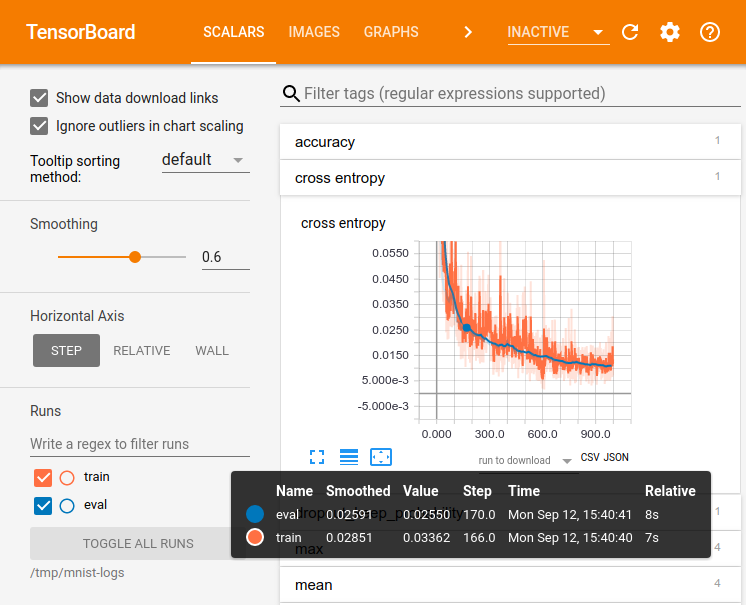
\includegraphics[width=\textwidth]{mnist_tensorboard.png}
% \caption{MNIST的TensorBoard图}
% \end{figure}
% 这个导航尝试让你从简单的TensorBoard开始。其它的资源也可用。\href{https://github.com/tensorflow/tensorboard}{TensorBoard's Github}有一些关于TensorBoard的使用,包含技巧,注意和调试信息。
% 
% \subsection{序列化数据}
% TensorBoard操作通过读TensorBoard包含TensorFlow运行产生的事件文件。时间文件的通常声明周期在TensorBoard中。
% 
% 首先创建TensorFlow图收集你想总结的数据,决定你想用\href{https://www.tensorflow.org/api_guides/python/summary}{summary operations}的那个节点。
% 
% 例如,假设你正在训练一个卷积神经网络识别MNIST数字。你想记录学习率变量随着时间如何变化,目标函数如何改变。通过添加\href{https://www.tensorflow.org/api_docs/python/tf/summary/scalar}{tf.summary.scalar }操作到节点输出学习率和损失的关系。然后给scalar\_summary一个有意义的tag,像`learning rate`或者`loss function`。
% 
% 也许你想可视化特殊层的分布,或者梯度或者权重的分布。通过\href{https://www.tensorflow.org/api_docs/python/tf/summary/histogram}{tf.summary.histogram}操作生成提出输出和和你的权重变量的对应关系。
% 
% 更多详细的总结操作查看\href{https://www.tensorflow.org/api_guides/python/summary}{summary operations}。
% 
% 在TensorFlow中的操作在你运行它之前将不做任何操作,或者一个操作依赖他们的输出。在你的图上创建的总结节点仅仅是次要的:你当前的操作没有任何一个依赖于他们。因此,生成总结,我们需要运行这些总结节点。手动管理这些节点将很愚蠢,为了使用\href{https://www.tensorflow.org/api_docs/python/tf/summary/merge_all}{tf.summary.merge\_all}结合他们在一个单独的操作生成所有的总结。
% 
% 然后你可以运行融合操作,生成给定步数的序列化的Summary protobuf对象。最后,为了写这个总结数据到磁盘,传递总结protobuf到一个\href{https://www.tensorflow.org/api_docs/python/tf/summary/FileWriter}{tf.summary.FileWriter}
% 
% FileWriter接受一个logdir,这个logdir很重要,它是所有时间输出的目录。FileWriter可以选择接受一个Graph构造体。如果它接受一个Graph对象,然后TensorBoard将沿着tensor形状可视化你的图。这将给你一个更好的理解你的图。查看\href{https://www.tensorflow.org/programmers_guide/graph_viz#tensor-shape-information}{Tensor shape information}
% 
% 注意你已经修改了你的图有一个FileWriter,你准备好了运行你的网络!如果你想,你可以单步运行融合操作,记录一些训练数据。这可能比你需要的多,因此考虑每n步运行融合的总结操作。
% 
% 下面的代码修改自\href{https://www.tensorflow.org/tutorials/layers}{simple MNIST tutorial},在代码中我们已经记录了总结和运行统计。查看\href{https://www.tensorflow.org/programmers_guide/summaries_and_tensorboard#serializing-the-data}{Summaries Tutorial}了解如何记录总结的详细信息。完整代码在\href{https://www.github.com/tensorflow/tensorflow/blob/r1.6/tensorflow/examples/tutorials/mnist/mnist_with_summaries.py}{这里}。
% \begin{pythoncode}
% # Train the model, and also write summaries.
%   # Every 10th step, measure test-set accuracy, and write test summaries
%   # All other steps, run train_step on training data, & add training summaries
% 
%   def feed_dict(train):
%     """Make a TensorFlow feed_dict: maps data onto Tensor placeholders."""
%     if train or FLAGS.fake_data:
%       xs, ys = mnist.train.next_batch(100, fake_data=FLAGS.fake_data)
%       k = FLAGS.dropout
%     else:
%       xs, ys = mnist.test.images, mnist.test.labels
%       k = 1.0
%     return {x: xs, y_: ys, keep_prob: k}
% 
%   for i in range(FLAGS.max_steps):
%     if i % 10 == 0:  # Record summaries and test-set accuracy
%       summary, acc = sess.run([merged, accuracy], feed_dict=feed_dict(False))
%       test_writer.add_summary(summary, i)
%       print('Accuracy at step %s: %s' % (i, acc))
%     else:  # Record train set summaries, and train
%       if i % 100 == 99:  # Record execution stats
%         run_options = tf.RunOptions(trace_level=tf.RunOptions.FULL_TRACE)
%         run_metadata = tf.RunMetadata()
%         summary, _ = sess.run([merged, train_step],
%                               feed_dict=feed_dict(True),
%                               options=run_options,
%                               run_metadata=run_metadata)
%         train_writer.add_run_metadata(run_metadata, 'step%d' % i)
%         train_writer.add_summary(summary, i)
%         print('Adding run metadata for', i)
%       else:  # Record a summary
%         summary, _ = sess.run([merged, train_step], feed_dict=feed_dict(True))
%         train_writer.add_summary(summary, i)
% \end{pythoncode}
% 这代码将每100在step99生成运行统计。
% 
% 当你启动tensorboard到Graph,你现在将在Session runs下看到运行metadada被添加的对应的步骤。选择一个运行将现实给你关于网络的快照,无用节点为灰色。在左边的控制面板,你将能着色memory或者总共的计算时间。例外,点击节点将显示准确的的memory,计算时间和tensor输出尺寸
% \begin{figure}[H]
% \centering
% 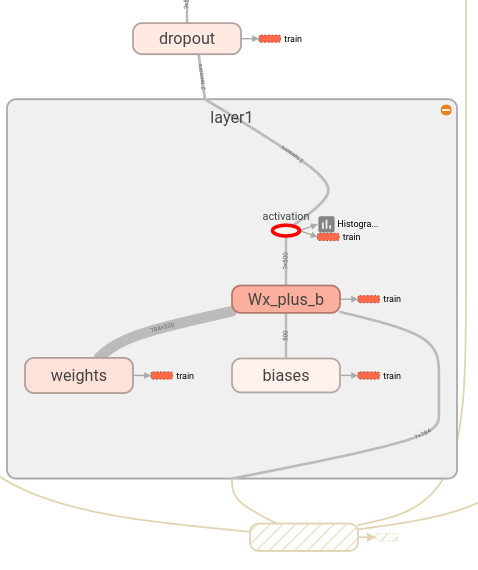
\includegraphics[width=\textwidth]{run_metadata_graph.png}
% \caption{MNIST的TensorBoard图}
% \end{figure}
\section{TensorBoard}
 \subsection{Visualizing Learning}\label{subsec:visualize}
 当你使用TensorFlow训练大规模深度神经网络的时候计算可能很复杂难以理解。为了更容易理解,调试,优化TensorFlow程序,我们包含了一个称为TensorBoard的可视化工具。你可以使用TensorBoard可视化你的TensorFlow图,画出关于你的图执行的一些度量,显示像图像之类的额外信息。TensorBoard配置好后看起来像这样:
 \begin{figure}[!ht]
 \centering
 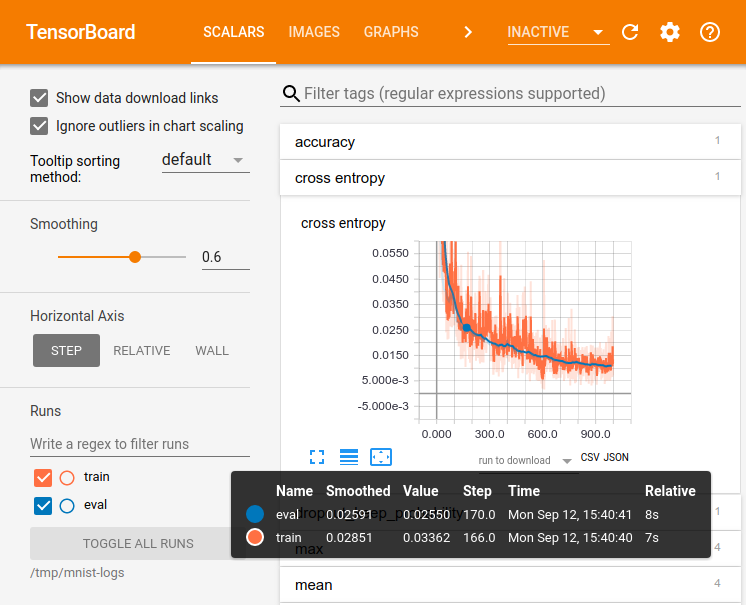
\includegraphics[width=\textwidth]{mnist_tensorboard.png}
 \caption{MNIST的TensorBoard图}
 \end{figure}
 这个导航尝试让你从简单的TensorBoard开始。其它的资源也可用。\href{https://github.com/tensorflow/tensorboard}{TensorBoard's Github}有一些关于TensorBoard的使用,包含技巧,注意和调试信息。
 
 \subsection{序列化数据}
 TensorBoard操作通过读TensorBoard包含TensorFlow运行产生的事件文件。时间文件的通常声明周期在TensorBoard中。
 
 首先创建TensorFlow图收集你想总结的数据,决定你想用\href{https://www.tensorflow.org/api_guides/python/summary}{summary operations}的那个节点。
 
 例如,假设你正在训练一个卷积神经网络识别MNIST数字。你想记录学习率变量随着时间如何变化,目标函数如何改变。通过添加\href{https://www.tensorflow.org/api_docs/python/tf/summary/scalar}{tf.summary.scalar }操作到节点输出学习率和损失的关系。然后给scalar\_summary一个有意义的tag,像`learning rate`或者`loss function`。
 
 也许你想可视化特殊层的分布,或者梯度或者权重的分布。通过\href{https://www.tensorflow.org/api_docs/python/tf/summary/histogram}{tf.summary.histogram}操作生成提出输出和和你的权重变量的对应关系。
 
 更多详细的总结操作查看\href{https://www.tensorflow.org/api_guides/python/summary}{summary operations}。
 
 在TensorFlow中的操作在你运行它之前将不做任何操作,或者一个操作依赖他们的输出。在你的图上创建的总结节点仅仅是次要的:你当前的操作没有任何一个依赖于他们。因此,生成总结,我们需要运行这些总结节点。手动管理这些节点将很愚蠢,为了使用\href{https://www.tensorflow.org/api_docs/python/tf/summary/merge_all}{tf.summary.merge\_all}结合他们在一个单独的操作生成所有的总结。
 
 然后你可以运行融合操作,生成给定步数的序列化的Summary protobuf对象。最后,为了写这个总结数据到磁盘,传递总结protobuf到一个\href{https://www.tensorflow.org/api_docs/python/tf/summary/FileWriter}{tf.summary.FileWriter}
 
 FileWriter接受一个logdir,这个logdir很重要,它是所有时间输出的目录。FileWriter可以选择接受一个Graph构造体。如果它接受一个Graph对象,然后TensorBoard将沿着tensor形状可视化你的图。这将给你一个更好的理解你的图。查看\href{https://www.tensorflow.org/programmers_guide/graph_viz#tensor-shape-information}{Tensor shape information}
 
 注意你已经修改了你的图有一个FileWriter,你准备好了运行你的网络!如果你想,你可以单步运行融合操作,记录一些训练数据。这可能比你需要的多,因此考虑每n步运行融合的总结操作。
 
 下面的代码修改自\href{https://www.tensorflow.org/tutorials/layers}{simple MNIST tutorial},在代码中我们已经记录了总结和运行统计。查看\href{https://www.tensorflow.org/programmers_guide/summaries_and_tensorboard#serializing-the-data}{Summaries Tutorial}了解如何记录总结的详细信息。完整代码在\href{https://www.github.com/tensorflow/tensorflow/blob/r1.6/tensorflow/examples/tutorials/mnist/mnist_with_summaries.py}{这里}。
 \begin{pythoncode}
 def variable_summaries(var):
   """Attach a lot of summaries to a Tensor (for TensorBoard visualization)."""
   with tf.name_scope('summaries'):
     mean = tf.reduce_mean(var)
     tf.summary.scalar('mean', mean)
     with tf.name_scope('stddev'):
       stddev = tf.sqrt(tf.reduce_mean(tf.square(var - mean)))
     tf.summary.scalar('stddev', stddev)
     tf.summary.scalar('max', tf.reduce_max(var))
     tf.summary.scalar('min', tf.reduce_min(var))
     tf.summary.histogram('histogram', var)
 
 def nn_layer(input_tensor, input_dim, output_dim, layer_name, act=tf.nn.relu):
   """Reusable code for making a simple neural net layer.
 
   It does a matrix multiply, bias add, and then uses relu to nonlinearize.
   It also sets up name scoping so that the resultant graph is easy to read,
   and adds a number of summary ops.
   """
   # Adding a name scope ensures logical grouping of the layers in the graph.
   with tf.name_scope(layer_name):
     # This Variable will hold the state of the weights for the layer
     with tf.name_scope('weights'):
       weights = weight_variable([input_dim, output_dim])
       variable_summaries(weights)
     with tf.name_scope('biases'):
       biases = bias_variable([output_dim])
       variable_summaries(biases)
     with tf.name_scope('Wx_plus_b'):
       preactivate = tf.matmul(input_tensor, weights) + biases
       tf.summary.histogram('pre_activations', preactivate)
     activations = act(preactivate, name='activation')
     tf.summary.histogram('activations', activations)
     return activations
 
 hidden1 = nn_layer(x, 784, 500, 'layer1')
 
 with tf.name_scope('dropout'):
   keep_prob = tf.placeholder(tf.float32)
   tf.summary.scalar('dropout_keep_probability', keep_prob)
   dropped = tf.nn.dropout(hidden1, keep_prob)
 
 # Do not apply softmax activation yet, see below.
 y = nn_layer(dropped, 500, 10, 'layer2', act=tf.identity)
 
 with tf.name_scope('cross_entropy'):
   # The raw formulation of cross-entropy,
   #
   # tf.reduce_mean(-tf.reduce_sum(y_ * tf.log(tf.softmax(y)),
   #                               reduction_indices=[1]))
   #
   # can be numerically unstable.
   #
   # So here we use tf.losses.sparse_softmax_cross_entropy on the
   # raw logit outputs of the nn_layer above.
   with tf.name_scope('total'):
     cross_entropy = tf.losses.sparse_softmax_cross_entropy(labels=y_, logits=y)
 tf.summary.scalar('cross_entropy', cross_entropy)
 
 with tf.name_scope('train'):
   train_step = tf.train.AdamOptimizer(FLAGS.learning_rate).minimize(
       cross_entropy)
 
 with tf.name_scope('accuracy'):
   with tf.name_scope('correct_prediction'):
     correct_prediction = tf.equal(tf.argmax(y, 1), tf.argmax(y_, 1))
   with tf.name_scope('accuracy'):
     accuracy = tf.reduce_mean(tf.cast(correct_prediction, tf.float32))
 tf.summary.scalar('accuracy', accuracy)
 
 # Merge all the summaries and write them out to /tmp/mnist_logs (by default)
 merged = tf.summary.merge_all()
 train_writer = tf.summary.FileWriter(FLAGS.summaries_dir + '/train',
                                       sess.graph)
 test_writer = tf.summary.FileWriter(FLAGS.summaries_dir + '/test')
 tf.global_variables_initializer().run()
 \end{pythoncode}
 % \begin{pythoncode}
 % # Train the model, and also write summaries.
 %   # Every 10th step, measure test-set accuracy, and write test summaries
 %   # All other steps, run train_step on training data, & add training summaries
 % 
 %   def feed_dict(train):
 %     """Make a TensorFlow feed_dict: maps data onto Tensor placeholders."""
 %     if train or FLAGS.fake_data:
 %       xs, ys = mnist.train.next_batch(100, fake_data=FLAGS.fake_data)
 %       k = FLAGS.dropout
 %     else:
 %       xs, ys = mnist.test.images, mnist.test.labels
 %       k = 1.0
 %     return {x: xs, y_: ys, keep_prob: k}
 % 
 %   for i in range(FLAGS.max_steps):
 %     if i % 10 == 0:  # Record summaries and test-set accuracy
 %       summary, acc = sess.run([merged, accuracy], feed_dict=feed_dict(False))
 %       test_writer.add_summary(summary, i)
 %       print('Accuracy at step %s: %s' % (i, acc))
 %     else:  # Record train set summaries, and train
 %       if i % 100 == 99:  # Record execution stats
 %         run_options = tf.RunOptions(trace_level=tf.RunOptions.FULL_TRACE)
 %         run_metadata = tf.RunMetadata()
 %         summary, _ = sess.run([merged, train_step],
 %                               feed_dict=feed_dict(True),
 %                               options=run_options,
 %                               run_metadata=run_metadata)
 %         train_writer.add_run_metadata(run_metadata, 'step%d' % i)
 %         train_writer.add_summary(summary, i)
 %         print('Adding run metadata for', i)
 %       else:  # Record a summary
 %         summary, _ = sess.run([merged, train_step], feed_dict=feed_dict(True))
 %         train_writer.add_summary(summary, i)
 % \end{pythoncode}
 在你初始化FileWriter后,你必须在训练和测试模型的时候添加总结到FileWriters。
 \begin{pythoncode}
 # Train the model, and also write summaries.
 # Every 10th step, measure test-set accuracy, and write test summaries
 # All other steps, run train_step on training data, & add training summaries
 
 def feed_dict(train):
   """Make a TensorFlow feed_dict: maps data onto Tensor placeholders."""
   if train or FLAGS.fake_data:
     xs, ys = mnist.train.next_batch(100, fake_data=FLAGS.fake_data)
     k = FLAGS.dropout
   else:
     xs, ys = mnist.test.images, mnist.test.labels
     k = 1.0
   return {x: xs, y_: ys, keep_prob: k}
 
 for i in range(FLAGS.max_steps):
   if i % 10 == 0:  # Record summaries and test-set accuracy
     summary, acc = sess.run([merged, accuracy], feed_dict=feed_dict(False))
     test_writer.add_summary(summary, i)
     print('Accuracy at step %s: %s' % (i, acc))
   else:  # Record train set summaries, and train
     summary, _ = sess.run([merged, train_step], feed_dict=feed_dict(True))
     train_writer.add_summary(summary, i)
 \end{pythoncode}
 你现在设置用TensorBoard可视化的所有数据。
 \subsection{启动TensorBoard}
 为了运行TensorBoard,使用下面的命令(或者python -m tensorboard.main)
 \mint{python}|tensorboard --logdir=path/to/log-directory|
 这里的logdir指定FileWriter序列化它的数据的目录。如果这logdir目录包含分开运行的子目录,TensorBoard将从所有的这些运行可视化。当TensorBoard运行的时候,导航你的web浏览器到localhost:6006查看TensorBoard。
 
 当查看TensorBoard,你将查看右上角的导航按钮,每个按钮代表可能被可视化的序列数据。
 
 更多深入的关于如何使用graph可视化你的图的信息,查看\href{https://www.tensorflow.org/programmers_guide/graph_viz}{TensorBoard:Graph Visualization}。
 
 更多在TensorBoard上的使用信息查看\href{https://github.com/tensorflow/tensorboard}{TensorBoard's Github}
\subsection{Graph 可视化} 
TensorFlow计算图很强大但是很复杂。图的可视化可以帮助你理解和调试他们。为了查看你的>图,运行TensorBoard指定job的采集目录,点击图上面板选择合适的运行。更多的关于如何运>行TensorBoard确保你采集所有需要的数据,查看\ref{subsec:visualize}
\subsection{名称scoping和nodes}
通常TensorFlow图可以有成千上万节点,多到甚至是用标准的绘图工具都难以查看,为了简化,变量名称可以被scoped和用图中的节点定义可视化信息。默认,仅仅显示层级结构。这里有一个例子在hidden scope下使用\href{https://www.tensorflow.org/api_docs/python/tf/name_scope}{tf.name\_scope}定义的hidden scope:
\begin{pythoncode}
import tensorflow as tf

with tf.name_scope('hidden') as scope:
  a = tf.constant(5, name='alpha')
  W = tf.Variable(tf.random_uniform([1, 2], -1.0, 1.0), name='weights')
  b = tf.Variable(tf.zeros([1]), name='biases')
\end{pythoncode}
下面的结果有三个操作名称:
\begin{itemize}
\item hidden/alpha
\item hidden/weights
\item hidden/biases
\end{itemize}
默认,可视化将压缩三个节点到一个hidden节点,详细信息没有丢失,双击橙色的+展开节点,然后你将看到子节点alpha,weights和biases。

这里是一个真实的立即展开的状态:
\begin{figure}[H]
\centering
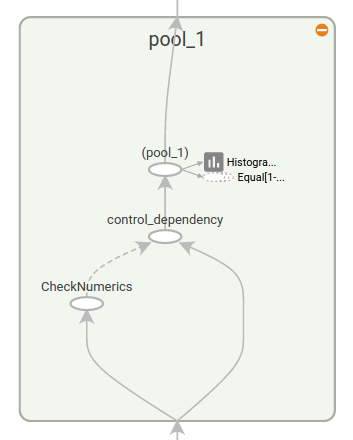
\includegraphics[width=0.5\textwidth]{pool1_expanded.png}
\caption{左边:pool\_1,右边:展开的内容}
\end{figure}
通过名字组合节点使得图更清晰。如果你构建一个模型,名称scope给你基于可视化之上的控制。你的名称scope越好,你的可视化越好。

上面的阐述可视化比率。TensorFlow图有两种连接:数据依赖和控制依赖。数据依赖显示两个操作之间的流,用实体箭头表示,控制依赖使用虚线箭头。在展开的视图(上图右)所有的连接是数据依赖结合虚线连接CheckNumerics和control\_dependencuies。

第二个简化布局的技巧。多数TensorFlow图有一些节点连接其他的节点。例如,一些节点也许在初始化的时候有一些控制依赖。画所有的边在init节点和他的依赖将看起来很杂乱。

为了减少咋暖,可视化分割所有的高级节点到右边的一个辅助区域没有画线代表他们的边。相对于先,我们话晓得节点图标表示连接。分割辅助节点步移除重要的信息,因此节点通常和bookkeeping函数相关。查看\href{https://www.tensorflow.org/programmers_guide/graph_viz#interaction}{Interaction}了解如何在主图和辅助区域移动节点。
\begin{figure}[H]
\centering
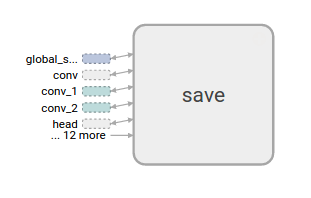
\includegraphics[width=0.5\textwidth]{save.png}
\caption{节点conv\_1连接到save,save为高级节点将在辅助区域显示}
\end{figure}
最后的结构简化是序列压缩。序列图,节点的名称有不同的数字结尾和同样的结构被压缩进一个简单的节点栈,正如下面显示。对于网络有唱的序列,这简化了试图。正如层叠节点,双击展开序列。查看\href{https://www.tensorflow.org/programmers_guide/graph_viz#interaction}{Interaction}了解如何禁用/开启层叠指定系列节点。
\begin{figure}[H]
\centering
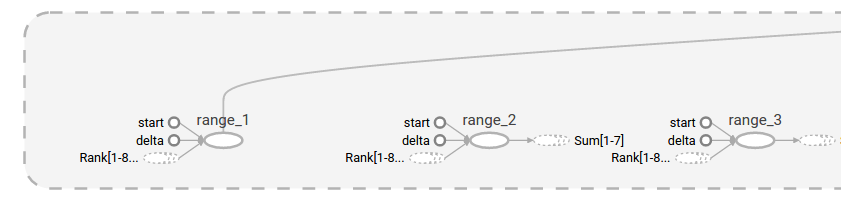
\includegraphics[width=0.5\textwidth]{series_expanded.png}
\caption{左边:压缩节点序列,右边:双击展开的视图}
\end{figure}
最后,可视化使用特殊的图标表示常数和总结节点。为了总结,这里有一些节点符号:b

\begin{table}[H]\label{fig:tensorboard_op}
\centering 
\begin{tabular}{|c|c|}
\hline
符号&含义\\
\hline 

\includegraphics{namespace_node.png}&高级节点表示一个name scope,双击展开节点\\
\hline

\includegraphics{horizontal_stack.png}&没有相互连接的序列节点\\
\hline

\includegraphics{vertical_stack.png}&相互连接的序列节点\\
\hline

\includegraphics{op_node.png}&一个单独的操作\\
\hline

\includegraphics{constant.png}&一个常数\\
\hline

\includegraphics{summary.png}&一个总结操作\\
\hline

\includegraphics{dataflow_edge.png}&显示数据在两个操作流动的边\\
\hline

\includegraphics{control_edge.png}&两个操作的控制依赖的边\\
\hline

\includegraphics{reference_edge.png}&参考边显示输出操作节点可以改变输入tensor\\
\hline
\end{tabular}
\end{table}
\subsection{交互}
通过缩放拖动图。点击或者拖动使用scroll缩放。双击在一个节点,或者点击+按钮,展开一个name scope表示操作集合。为了缩放的时候轻易地跟踪当前的视角,有一个minimap在右上角。

为了关闭一个开放的节点,双击它点击-按钮。你可以点击一次选择一个节点,它将变节点。它将编程灰色,详细的和节点连接将出现在右上角的信息card。
\begin{figure}[H]
\centering
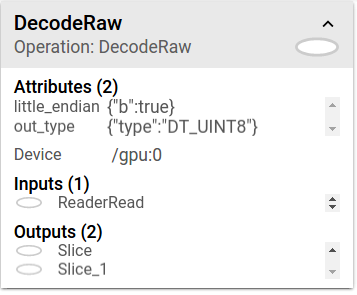
\includegraphics[width=0.5\textwidth]{infocard_op.png}
\caption{左边:信息卡显示conv2的名称scope。输入和输出结合scope的输入输出操作节点。右图:显示DecodeRaw操作的详细信息,额外的输入和输出,卡片显示设备和当前操作的属性}
\end{figure}
TensorBoard提供一些方法改变图的可视化布局。步改变图的计算语意学,但是它可以带来一些清晰地网络结构。通过右击节点的信息card节点,你可以做下面的布局更高:
\begin{itemize}
\item 节点可以在主图和辅助区域移动
\item 一些节点可以被解开组以至于在序列中的节点不出现在组中。解开组序列可以被重组。
\end{itemize}
选择可能在理解高级节点上很有用。选择任何高级节点,对应的节点图标对于其他连接将也被选中。这使得它很容易,例如,查看每个正在被保存的节点或者没有保存的。

点击一个信息卡片上节点名称。如果需要,视角将自动缩放以至于节点可视。

最后,你可以为你的图选择两种颜色方案,使用上面的颜色菜单。默认的结构视图:当两个高级节点有相同的结构时,他们出现在彩虹色中的同样颜色。特别的结构节点是灰色的。有第二个视图显示在不同设备上运行的操作。名称scope颜色比例被按不同设备分开着色。

下面的图给定一个真实图的细节:
\begin{figure}[H]
\centering
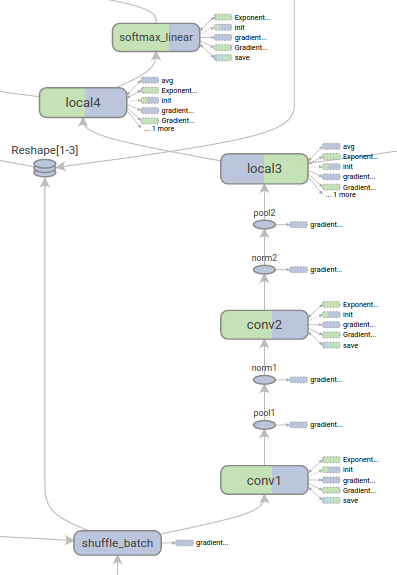
\includegraphics[width=0.5\textwidth]{colorby_device.png}
\caption{结构视图:灰色节点有特殊结构,橙色conv1和conv2节点有同样的结构,其他颜色节点类似。设备视图:名称scope分开着色不同设备上的操作,紫色为GPU绿色为CPU}
\end{figure}
\subsection{Tensor形状信息}
当序列的GraphDef包含tensor形状,图可视化器用tensor的维度标记边,边的宽反映了tensor的大小。为了包含tensor形状在GraphDef当序列化图的时候传递实际的图对象(正如在sess.graph)到FileWriter。下图显示CIFAR-10模型的tensor形状信息:
\begin{figure}[H]
\centering
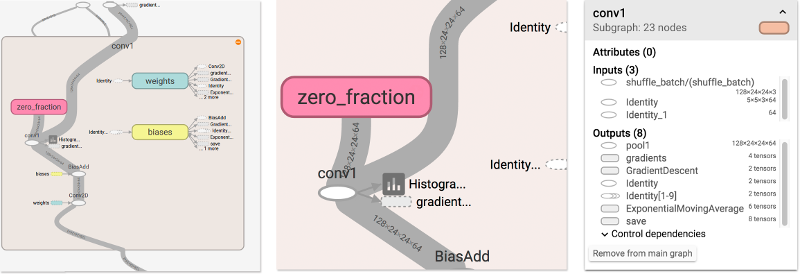
\includegraphics[width=0.5\textwidth]{tensor_shapes.png}
\caption{CIFAR-10模型的tensor信息}
\end{figure}
\subsection{运行统计}
经常为运行收集一些运行时的信息是有用的,想总内存使用,总计算时间,节点的tensor形状。下面的示例代码是\href{simple MINST tutorial}{https://www.tensorflow.org/tutorials/layers}的片段,在代码中我们记录了总结和运行统计。查看\href{https://www.tensorflow.org/programmers_guide/summaries_and_tensorboard#serializing-the-data}{Summary Tutorial}了解如何记录总结的详细信息。完整的源代码在\href{https://www.github.com/tensorflow/tensorflow/blob/r1.6/tensorflow/examples/tutorials/mnist/mnist_with_summaries.py}{这里}
\begin{pythoncode}
# Train the model, and also write summaries.
  # Every 10th step, measure test-set accuracy, and write test summaries
  # All other steps, run train_step on training data, & add training summaries

  def feed_dict(train):
    """Make a TensorFlow feed_dict: maps data onto Tensor placeholders."""
    if train or FLAGS.fake_data:
      xs, ys = mnist.train.next_batch(100, fake_data=FLAGS.fake_data)
      k = FLAGS.dropout
    else:
      xs, ys = mnist.test.images, mnist.test.labels
      k = 1.0
    return {x: xs, y_: ys, keep_prob: k}

  for i in range(FLAGS.max_steps):
    if i % 10 == 0:  # Record summaries and test-set accuracy
      summary, acc = sess.run([merged, accuracy], feed_dict=feed_dict(False))
      test_writer.add_summary(summary, i)
      print('Accuracy at step %s: %s' % (i, acc))
    else:  # Record train set summaries, and train
      if i % 100 == 99:  # Record execution stats
        run_options = tf.RunOptions(trace_level=tf.RunOptions.FULL_TRACE)
        run_metadata = tf.RunMetadata()
        summary, _ = sess.run([merged, train_step],
                              feed_dict=feed_dict(True),
                              options=run_options,
                              run_metadata=run_metadata)
        train_writer.add_run_metadata(run_metadata, 'step%d' % i)
        train_writer.add_summary(summary, i)
        print('Adding run metadata for', i)
      else:  # Record a summary
        summary, _ = sess.run([merged, train_step], feed_dict=feed_dict(True))
        train_writer.add_summary(summary, i)
\end{pythoncode}
这段代码每100步发送运行统计,在step99时发送。当你启动tensorboard和其他的Graph tab,你将现在查看选项"Session runs",它对应运行meta被添加的步骤。选择一个运行将给你显示这一步网络的快照,隐去无用的节点。在左边的控制区域,你将能通过统计计算时间着色节点。另外,检查节点将显示总共的内存,计算时间和tensor输出大小。
\begin{figure}[H]
\centering
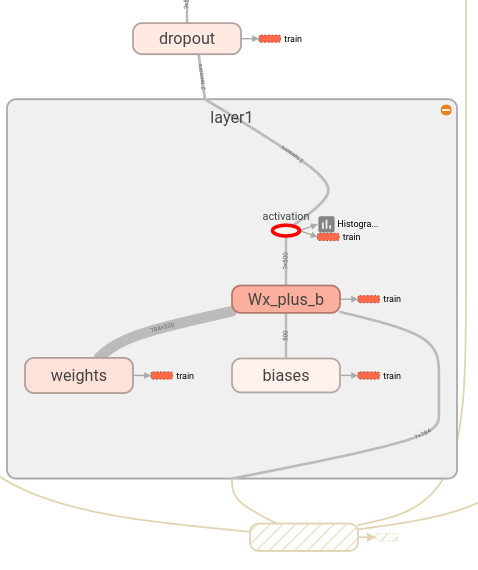
\includegraphics[width=0.5\textwidth]{run_metadata_graph.png}
\end{figure}


 % 当你启动tensorboard到Graph,你现在将在Session runs下看到运行metadada被添加的对应的步骤。选择一个运行将现实给你关于网络的快照,无用节点为灰色。在左边的控制面板,你将能着色memory或者总共的计算时间。例外,点击节点将显示准确的的memory,计算时间和tensor输出尺寸
 % \begin{figure}[!ht]
 % \centering
 % 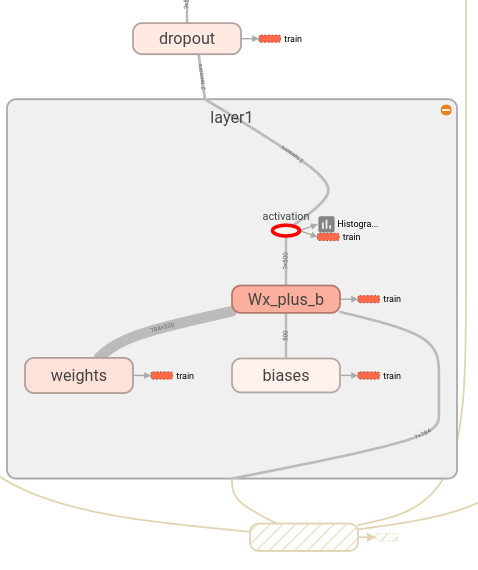
\includegraphics[width=\textwidth]{run_metadata_graph.png}
 % \caption{MNIST的TensorBoard图}
 % \end{figure}
 


\subsection{TensorBoard Histogram Dashboard}

TensorBoard Histogram Dashboard 显示TensorFlow图中的Tensor如何随着时间变化。
\subsection{一个简单的例子}
正态分布变量,均值随着和时间移动。TensorFlow有一个操作tf.random\_normal可以完美的达到这个目的。正如通常情况下TensorBoard,我们将用summary op融合数据据。
在这种情况下'tf.summary.histogram'。
这里有一个代码段将生成一些包含正态分布直方图数据的总结,这里均值随着时间增大。
\begin{lstlisting}[language=Python]
import tensorflow as tf
k = tf.placeholder(tf.float32)
mean_moving_normal = tf.random_normal(shape=[1000], mean=(5*k), stddev=1)
summaries = tf.summary.histogram('normal/moving_mean',mean_moving_normal)
sess = tf.Session()
writer = tf.summary.FileWriter('./histogram_example')
N = 400
for step in range(N):
    k_val = step/float(N)
    summ = sess.run(summaries,feed_dict={k:k_val})
    writer.add_summary(summ,global_step=step)
\end{lstlisting}
在当前代码中运行下边的代码启动TensorFlow载入数据
\begin{lstlisting}[language=Python]
tensorboard --logdir=./histogram_example
\end{lstlisting}
\begin{center}
\begin{figure}[H]
\includegraphics[width=\textwidth]{tb_hist1.png}
\end{figure}
\end{center}
tf.summary.histogram接受任一尺寸和大小的Tensor,压缩它们进入直方数据结构组成一些小的数据宽度和数量组层的bin将诶够,例如我们像组成数[0.5,1.1,1.3,2.2,2.9,2.99]成3个bin,我们可以创建三个bin:一个包含0到1之间的一切(0.5),一个包含1-2(1.1,1.3)之间,一个包含2-3(2.2,2.9,2.99)

  TensorFlow用类是的方法创建bins,但是不像我们上面的例子,它不创建整数读额bins,瑞与大型数据,稀疏数据,这样的也许导致上千个bin,bins时指数分布时,一些bins相比于一些非常大数的bin接近于0。然而,可视化指数分布bin时一个技巧,如果高被编码为数量,bin宽度更大的空间,甚至它们有相同的元素,相比较之下统计数量使得豪赌比较变得可能,直方图采集数据仅均匀的bins,这可能导致不幸的人工操作。

在直方图可视化器的每一个切片显示为一个单个的直方图。切片安装步数组织。例老的切片(e.g. step 0)比较靠后变为更深,然而新的slices接近于前景色,颜色更轻,右边的y轴显示了步数。

你可以在直方图上滑动鼠标看到更多的详细星系。你如下面的图你可以看到直方图的时间不为177有一个bin中心在3.78有bin中有34.5个元素。
\begin{center}
\begin{figure}[H]
\includegraphics[width=\textwidth]{tb_hist2.png}
\end{figure}
\end{center}
你也许注意到注意到直方切片在统计步数和时间上不总是偶数,这是因为TensorBoard用\href{https://en.wikipedia.org/wiki/Reservoir\_sampling}{reservoir sampling}保持直方图的子集,为了节约内存,Reservior sampling保证每个采样有一个相等的可能性被包含进去,但是因为它时一个随机算法,采样并不在每个偶数步发生。
\subsection{Overlay Mode}
控制面板上允许你打开直方图模式为offset为overlay。
在offset模式下,可视化转动45度,因此单个的直方图切片不再展开,而是所有的图华仔一个相同的y轴上。
\begin{center}
\begin{figure}[H]
\includegraphics[width=\textwidth]{tb_hist3.png}
\end{figure}
\end{center}
现在表上的每个切片被线分开,y轴显示每个bucket项目数量,深色线时老的,早期的时间不,浅色线时最近的新的时间不,你可以用鼠标在表上查看更多的信息。
\begin{center}
\begin{figure}[H]
\includegraphics[width=\textwidth]{tb_hist4.png}
\end{figure}
\end{center}

overlay可视化在你想直接比较不同直方图的数量。
\subsection{多个分布}
直方图控制面板对多分布下的可视化很有用,当我们通过链接两个不同的正态分布构造一个简单的二两分布,代码如下:
\begin{lstlisting}[language=Python]
import tensorflow as tf
k = tf.placeholder(tf.float32)
mean_moving_normal = tf.random_normal(shape=[1000],mean=(3*5),stddev=1)
tf.summary.histogram('normal/moving_mean',mean_moving_normal)
variance_shrinking_normal = tf.random_normal(shape=[100],mean=0,stddev=1-(k))
tf.summary.histogram('normal/shrinking_varance',variance_shrinking_normal)
normal_combined = tf.concat([mean_moving_normal,variance_shrinking_normal],0)
tf.summary.histogram('normal/bimodal',normal_combined)
summaris = tf.summary.merge_all()
sess = tf.Session()
writer = tf.summary.FileWriter('./histgram_example1')
N = 400
for step in range(N):
    k_val = step/float(N)
    summ = sess.run(summaris,feed_dict={k:k_val})
    writer.add_summary(summ,global_step=step)
\end{lstlisting}
上面的例子是滑动平均,现在我们已有一个收缩的变量分布。
\begin{center}
\begin{figure}[H]
\includegraphics[width=\textwidth]{tb_hist5.png}
\end{figure}
\end{center}
当我们链接她们在一起,我们得到一个清晰解释分歧,二进制结构的表格:
\begin{center}
\begin{figure}[H]
\includegraphics[width=\textwidth]{tb_hist6.png}
\end{figure}
\end{center}
\subsection{更多分布}
生成可视化更多分布,结合它们到表中:
\begin{lstlisting}[language=Python]
import tensorflow as tf
k = tf.placeholder(tf.float32)
# Make a normal distribution,with a shift mean
mean_moving_normal = tf.random_normal(shape=[1000],mean=(5*k),stddev=1)
tf.summary.histogram('normal/moving_mean',mean_moving_normal)
variance_shrinking_normal = tf.random_normal(shape=[1000],mean=0,stddev=1-(k))
tf.summary.histogram('normal/shinking_variance',variance_shrinking_normal)
normal_combined = tf.concat([mean_moving_normal,variance_shrinking_normal],0)
tf.summary.histogram("normal/bimodal",normal_combined)
#add gamma distribution
gamma = tf.random_gamma(shape=[1000],alpha=k)
tf.summary.histogram('gamma',gamma)
poisson = tf.random_poisson(shape=[1000],lam=k)
tf.summary.histogram('poisson',poisson)
#add a uniform distribution
uniform = tf.random_uniform(shape=[1000],maxval=k*10)
tf.summary.histogram('uniform',uniform)
#finnally combine everything together

all_distributions = [mean_moving_normal,variance_shrinking_normal,gamma,poisson,uniform]
all_combined = tf.concat(all_distributions,0)
tf.summary.histogram('all_combined',all_combined)
summaries = tf.summary.merge_all()
sess = tf.Session()
writer = tf.summary.FileWriter('./histogram_example2')
N = 400
for step in range(N):
    k_val = step/float(N)
    summ = sess.run(summaries,feed_dict={k:k_val})
    writer.add_summary(summ,global_step=step)
\end{lstlisting}
\begin{center}
\begin{figure}[H]
\includegraphics[width=\textwidth]{tb_hist7.png}
\end{figure}
\end{center}
\begin{center}
\begin{figure}
\includegraphics[width=\textwidth]{tb_hist9.png}
\end{figure}
\end{center}
\subsection{poisson分布}
\begin{center}
\begin{figure}[H]
\includegraphics[width=\textwidth]{tb_hist10.png}
\end{figure}
\end{center}
poisson分布定义在整数上,因此所有被生成的值都是整数,直方图压缩移动数据到浮点bins,导致可视化在整数值上显示一点点突起。
\subsection{结合所有的数据到一张图向上}
\begin{center}
\begin{figure}[H]
\includegraphics[width=\textwidth]{tb_hist11.png}
\end{figure}
\end{center}


\begin{lstlisting}[language=Python]
import tensorflow as tf
import matplotlib.pyplot as plt
import numpy as np
tf.set_random_seed(0)
np.random.seed(0)
x = np.linspace(-1,1,100).reshape(-1,1)
noise = np.random.normal(0,0.1,size=x.shape)
y = np.power(x,2)+noise
def gendata():
    t = np.linspace(-1,1,100).reshape(-1,1)
def save():
    print('This is save')
    tf_x = tf.placeholder(tf.float32,x.shape)
    tf_y = tf.placeholder(tf.float32,y.shape)
    l = tf.layers.dense(tf_x,10,tf.nn.relu)
    o = tf.layers.dense(l,1)
    loss = tf.losses.mean_squared_error(tf_y,o)
    train_op = tf.train.GradientDescentOptimizer(learning_rate=0.5).minimize(loss)
    sess = tf.Session()
    sess.run(tf.global_variables_initializer())
    saver = tf.train.Saver()
    for step in range(100):
        sess.run(train_op,{tf_x:x,tf_y:y})
    saver.save(sess,'params',write_meta_graph=False)
    pred,l = sess.run([o,loss],{tf_x:x,tf_y:y})
    plt.figure(1,figsize=(10,5))
    plt.subplot(121)
    plt.scatter(x,y)
    plt.plot(x,pred,'r-',lw=5)
    plt.text(-1,1.2,'save loss=%.4f'%l,fontdict={'size':15,'color':'red'})
def reload():
    print('This is reload')
    tf_x = tf.placeholder(tf.float32,x.shape)
    tf_y = tf.placeholder(tf.float32,y.shape)
    l_ = tf.layers.dense(tf_x,10,tf.nn.relu)
    o_ = tf.layers.dense(l_,1)
    loss_ = tf.losses.mean_squared_error(tf_y,o_)
    sess = tf.Session()
    saver = tf.train.Saver()
    saver.restore(sess,'params')
    pred,l = sess.run([o_,loss_],{tf_x:x,tf_y:y})
    plt.subplot(122)
    plt.scatter(x,y)
    plt.plot(x,pred,'r-',lw=5)
    plt.text(-1,1.2,'Reload Loss=%.4f'%l,fontdict={'size':15,'color':'red'})
    plt.show()
save()
tf.reset_default_graph()
reload()
\end{lstlisting}

\chapter{程序员向导}
\section{Estimators}
这篇文章介绍简化机器学习程序的高级TensorFlow API\href{https://www.tensorflow.org/api_docs/python/tf/estimator?hl=zh-cn}{ Estimators }。Estimator封装下面的行为:
\begin{itemize}
\item training
\item evaluation
\item prediction
\item export for serving
\end{itemize}
你既可以用我们提供的预先定义好的Estimator也可以写你自己的自定义的Estimator。所有的自定义的或预先提供的Estimators都基于\href{https://www.tensorflow.org/api_docs/python/tf/estimator/Estimator?hl=zh-cn}{tf.estimator.Estimator}类。
\begin{quote}
注意:TensorFlow在\href{https://www.tensorflow.org/api_docs/python/tf/contrib/learn/Estimator?hl=zh-cn}{tf.contrib.learn.Estimator }包含一个你不应该使用的废弃的Estimator。
\end{quote}
\subsection{高级Estimator}
Estimators提供下面的好处:
\begin{itemize}
\item 你可以不用改变你的模型在本地主机或者多服务器环境下运行Estimator-based。更进一步,你可以在CPU,GPU或者没有记录你的模型的TPU运行Estimator-base的模型
\item Estimators简化了模型开发者回见的共同实现
\item 你可以用高级直接代码开发一个艺术模型的状态,简单来讲,通常用Estimator创建模型比TensorFlow低级API要更简单。
\item Estimators本身构建在简化自定义的tf.layers中
\item Estimators为你构建一个图。换句话说,你不用构件图
\item Estimator提供了一个安全的分布式的训练循环控制如何或者什么时候做:
\begin{itemize}
\item 构建图
\item 初始化变量
\item 开始队列
\item 处理异常
\item 创建checkpoint文件并且从失败中恢复
\item 为TensorBoard保存总结文件
\end{itemize}
\end{itemize}
当用Estimator写一个应用时,你必须从模型中分开输入pipeline。分开简化了在不同数据集上的试验。
\subsection{自定义的Estimator}
自定义的Estimator使得你能在高于TensorFlow APIs的高级概念级别上工作。你不用担心创建计算图和会话因为Estimator为你处理所有的plubmbing。预定义的Estimator为你创建管理\href{https://www.tensorflow.org/api_docs/python/tf/Graph?hl=zh-cn}{图}和\href{https://www.tensorflow.org/api_docs/python/tf/Session?hl=zh-cn}{会话}对象。进一步,预定义的Estimators让你做最小的代码改动结合不同的模型架构试验。\href{https://www.tensorflow.org/api_docs/python/tf/estimator/DNNClassifier?hl=zh-cn}{DNNClassfier},例如一个自定义的Estimators类通过dense,前馈神经网络训练分类模型。
\subsection{预定义的Estimator程序结构}
一个预先定义的Estimator的TensorFlow程序通常由四步组成:
\begin{enumerate}
\item 写一个或者更多的数据集导入函数。例如也许创建一个函数导入训练集创建另一个函数导入测试集。每个数据集导入函数必须有两个对象:
\begin{itemize}
\item 一个包含对应特征数据的key为特征名字的value是Tensor的词典
\item 一个Tensor包含一个或者更多标签\newline
例如,下面的代码吧、描述了基本的输入函数框架:
\begin{lstlisting}[language=Python]
def input_fn(dataset):
   ...  # manipulate dataset, extracting feature names and the label
   return feature_dict, label
\end{lstlisting}
(查看\href{https://www.tensorflow.org/programmers_guide/datasets?hl=zh-cn}{Importing Data}获取详细信息)
\end{itemize}
\item 定义特征列。每个\href{https://www.tensorflow.org/api_docs/python/tf/feature_column?hl=zh-cn}{tf.feature\_column}确定特征名字,它的类型和输入预处理。例如,下面的的代码创建三个包含整数和浮点数据的特征列。三个特征列也指定一个lambda程序调用原始数据的缩放:\newline
\begin{lstlisting}[language=Python]
# Define three numeric feature columns.
population = tf.feature_column.numeric_column('population')
crime_rate = tf.feature_column.numeric_column('crime_rate')
median_education = tf.feature_column.numeric_column('median_education',
                    normalizer_fn='lambda x: x - global_education_mean')
\end{lstlisting}
\item 实例化相关的预定义Estimator。例如有一个预先定义的名字为LinearClassfier 的Estimator实现:
\begin{lstlisting}[language=Python]
# Instantiate an estimator, passing the feature columns.
estimator = tf.estimator.Estimator.LinearClassifier(
    feature_columns=[population, crime_rate, median_education],
    )
\end{lstlisting}

\item 调用一个训练,评估,推理方法。例如,所有的Estimator提供一个训练方法训练模型。\newline
\begin{lstlisting}[language=Python]
# my_training_set is the function created in Step 1
estimator.train(input_fn=my_training_set, steps=2000)
\end{lstlisting}
\end{enumerate}
\subsection{预定义Estimators的好处}
预定义的Estimators编码最佳实践提供下面的好处:
\begin{itemize}
\item 最佳决定不同计算图的不同部分应该运行在单台机器或者集群上实现方案的实践
\item 最佳事件(总结)和普遍的有用的总结时间
\end{itemize}
如果你不用自定义的Estimator,你自己必须实现上面的特征。
\subsection{自定义Estimators}
每个Estimator(预定义或者是自定义)的核心是模型函数,它包含了构建训练,评估,预测图的方法。然后当你使用一个预定义的Estimator有些人已经实现了模型函数,当依赖一个自定义的Estimator时,你必须自己写模型函数。一个\href{https://www.tensorflow.org/extend/estimators?hl=zh-cn}{ companion document }解释如何写一个模型函数。
\subsection{推荐的工作流程}
推荐的工作流程如下:
\begin{enumerate}
\item 假设存在一个合适的预定义的Estimator,用它构建你的第一个模型,用它的结果建立一个baseline
\item 构建测试你的pipeline,包含使用这个预定义的Estimator的关于你的数据的完整性和真实性
\item 如果合适的Estimator可用,运行试验决定哪个pre-made Estimator产生最好的结果
\item 可能的话,进一步提高你的模型构建你自定义的Estimator
\end{enumerate}
\subsection{从Keras模型创建Estimator}
你可以转化已经存在的Keras模型为Estimator。这样做能使得你的Keras模型获得Estimator‘s的力量,像分布式的训练。如下面样例调用\href{https://www.tensorflow.org/api_docs/python/tf/keras/estimator/model_to_estimator?hl=zh-cn}{ tf.keras.estimator.model\_to\_estimator}
\begin{lstlisting}[language=Python]
# Instantiate a Keras inception v3 model.
keras_inception_v3 = tf.keras.applications.inception_v3.InceptionV3(weights=None)
# Compile model with the optimizer, loss, and metrics you'd like to train with.
keras_inception_v3.compile(optimizer=tf.keras.optimizers.SGD(lr=0.0001, momentum=0.9),
                          loss='categorical_crossentropy',
                          metric='accuracy')
# Create an Estimator from the compiled Keras model.
est_inception_v3 = tf.keras.estimator.model_to_estimator(keras_model=keras_inception_v3)
# Treat the derived Estimator as you would any other Estimator. For example,
# the following derived Estimator calls the train method:
est_inception_v3.train(input_fn=my_training_set, steps=2000)
\end{lstlisting}
更多细节查看\href{https://www.tensorflow.org/api_docs/python/tf/keras/estimator/model_to_estimator?hl=zh-cn}{tf.keras.estimator.model\_to\_estimator }。
\section{Tensor}
Tensorflow正如它的名字表达的一样是定义tensor的计算。一个tensor是一个概括的矩阵和向量,并且有能力表示更高的维度,我们写Tensorflow程序,主要的对象就是tf.Tensor,一个tensor定义计算的一部分,最后生成值。TensorFlow程序首先用tensor建立一个图,然后运行图获得想要的数据。一个tensor需要指定两个参数:数据类型和形状。Tensor中的数据类型相同,而且总是可知的,形状可能仅仅部分知道。
下面是一些特殊的Tensor类型:
\begin{itemize}
\item	tf.Variable
\item	tf.Constant
\item	tf.Placeholder
\item	tf.SparseTensor
\end{itemize}
\subsection{Rank}
tf.Tensor的rank是对象的维度。TensorFlow的rank和数学中矩阵的rank不一样,下面显示TensorFlow rank和相对应的数学实体
\begin{center}
\begin{tabular}{|c|c|}
\hline
rank&数学实体\\
\hline
0&Scalar(只有值)\\
\hline
1&Vecor(值和方向)\\
\hline
2&矩阵(数值表)\\
\hline
3&3-Tensor\\
\hline
n&n-Tensor\\
\hline
\end{tabular}
\end{center}
\textbf{Rank0}

下面片段展示创建一些0维的变量。
\begin{lstlisting}[language=Python]
mammal = tf.Variable("Elephant", tf.string)
ignition = tf.Variable(451, tf.int16)
floating = tf.Variable(3.14159265359, tf.float64)
its_complicated = tf.Variable((12.3, -4.85), tf.complex64)
\end{lstlisting}
\textbf{Rank1}
传递列表作为初始值创建1维tf.Tensor对象
\begin{lstlisting}[language=Python]
mystr = tf.Variable(["Hello"], tf.string)
cool_numbers  = tf.Variable([3.14159, 2.71828], tf.float32)
first_primes = tf.Variable([2, 3, 5, 7, 11], tf.int32)
its_very_complicated = tf.Variable([(12.3, -4.85), (7.5, -6.23)], tf.complex64)
\end{lstlisting}
\textbf{更高的rank:}
二维的Tensor至少有一行一列
\begin{lstlisting}[language=Python]
mymat = tf.Variable([[7],[11]], tf.int16)
myxor = tf.Variable([[False, True],[True, False]], tf.bool)
linear_squares = tf.Variable([[4], [9], [16], [25]], tf.int32)
squarish_squares = tf.Variable([ [4, 9], [16, 25] ], tf.int32)
rank_of_squares = tf.rank(squarish_squares)
mymatC = tf.Variable([[7],[11]], tf.int32)
\end{lstlisting}
更高rank的Tensor,有n维数组。例如在图像处理,一些tensor的rank为4,维度通常是example-in-batch,image width,image height,color chennel。
\begin{lstlisting}[language=Python]
my_image = tf.zeros([10, 299, 299, 3])  # batch x height x width x color
\end{lstlisting}
\subsection{获取Tensor对象的rank}
你可以使用tf.rank方法获取tensor对象的rank。例如下面获取my3d的rank。
\begin{lstlisting}[language=Python]
r = tf.rank(my3d)	#在图运行后,r将保持值3。
\end{lstlisting}
\subsection{Tensor的切片}
因为tf.Tensor是n维cell阵列,为了访问tf.Tensor的单个cell,你需要指定索引。
对于rank为0的tensor,不需要索引,因为它已经是单个值了。\par
对于rank1(向量),传递一个索引允许你访问:
\begin{lstlisting}[language=Python]
my_scale = my_vector[2]
\end{lstlisting}
如果你想动态的选择向量中的元素,你可以指定[]获取一个tf.Tensor。
传递一个数值访问矩阵的子向量:
\begin{lstlisting}[language=Python]
my_row_vetor = my_matrix[2]
my_column_vector = my_matrix[:, 3]
\end{lstlisting}
\subsection{形状}
shape是tensor每一维元素的个数。TensorFlow在构造图的时候自动计算形状。有时候自动计算可能不知道rank,如果rank已经知道,每一维的形状可能知道可能不知道。
\begin{table}[H]\label{tb:pro1}
\centering
\begin{tabular}{|c|c|c|c|}
\hline
rank&shape&维数&example\\
\hline
0&[ ]&0-D&O维Tensor,标量\\
\hline
1&[D0]&1-D&一维tensor的形状\\
\hline
2&[D0,D1]&2-D&二维Tensoe的形状\\
\hline
3&[D0,D1,D2]&3-D&三维Tensor的形状\\
\hline
n&[D0,D1,\ldots,$D_{n-1}$]&N维tensor的形状[$D_0,D_1,\ldots,D_{n-1}$]&\\
\hline
\end{tabular}
\end{table}
\subsection{获取tf.Tensor对象的形状}
当建立图的时候tensor的形状已知是很有用的,你可以通过tensor的shape属性得到它的形状。得到完全定义的tf.Tensor的形状可以使用tf.shape操作。这个方法你可以建立一个图操作tensor的形状。

例如,这里显示如何创建一个和给定矩阵列数相同的全零向量。
\begin{lstlisting}[language=Python]
zeros = tf.zeros(tf.shape(my_matrix)[1])
\end{lstlisting}
\subsection{改变Tensor的形状}
tensor的元素个数是所有形状值的乘积。标量的元素形状总是1.因此,因为有相同元素不同形状的tensor,转变它们的形状是很方便的。可以使用tf.reshape.

下面例子展示了如何reshape tensor。
\begin{lstlisting}[language=Python]
rank_three_tensor = tf.ones([3, 4, 5])
matrix = tf.reshape(rank_three_tensor, [6, 10])  # Reshape existing content into
                                                 # a 6x10 matrix
matrixB = tf.reshape(matrix, [3, -1])  #  Reshape existing content into a 3x20
                                       # matrix. -1 tells reshape to calculate
                                       # the size of this dimension.
matrixAlt = tf.reshape(matrixB, [4, 3, -1])  # Reshape existing content into a
                                             #4x3x5 tensor

# Note that the number of elements of the reshaped Tensors has to match the
# original number of elements. Therefore, the following example generates an
# error because no possible value for the last dimension will match the number
# of elements.
yet_another = tf.reshape(matrixAlt, [13, 2, -1])  # ERROR!
\end{lstlisting}
\subsection{数据类型}
tf.Tensor不可能有一个以上的数据类型。然而序列化任意数据结构作为字符串存储在tf.Tensor里是可能的。

可以使用tf.cast转换一种数据类型到另一种。
\begin{lstlisting}[language=Python]
# Cast a constant integer tensor into floating point.
float_tensor = tf.cast(tf.constant([1, 2, 3]), dtype=tf.float32)
\end{lstlisting}
通过Tensor的dtype查看tensor的数据类型。你通过python对象创建tf.Tensor的时候需要指定数据类型。如果你不指定TensorFlow选择一个代表你数据的数据类型。TensorFlow转换Python整数为tf.int32,浮点数为tf.float32。转换数组时TensorFlow用和numpy相同的规则。
\subsection{评价Tensor}
当计算图被创建后你可以通过运行计算tf.Tensor获取指定的值。用Tensor.eval方法简单的计算:
\begin{lstlisting}[language=Python]
sess = tf.Session()
constant = tf.constant([1,2,3])
tensor = constant*constant
print(tensor.eval(session=sess))
\end{lstlisting}
eval方法仅仅当tf.Session()被激活时可用。Tensor.eval然后会得到一个和tensor相同数据类型的numpy数组。有时候没有上下文计算tf.Tensor是不可能的。例如,tensor依赖于Placeholder在提供给Placeholder值之前不能计算。
\begin{lstlisting}[language=Python]
p = tf.placeholder(tf.float32)
t = p + 1.0
t.eval()  # This will fail, since the placeholder did not get a value.
t.eval(feed_dict={p:2.0})  # This will succeed because we're feeding a value
                           # to the placeholder.
\end{lstlisting}
其它的模型结构在计算tf.Tensor时可能很复杂。TensorFlow不能直接计算定义在函数内部的或者控制流结构的tf.Tensor。如果tf.Tensor依赖于队列中的值,计算tf.Tensor仅仅入队的时候工作,负责计算被挂起。当和queue工作的时候,记得在计算任何tf.Tensor之前用tf.train.start\_queue\_runners。
\subsection{打印Tensor}
出于调试目的,你想要打印tf.Tesor的值。tfdbg提供了高级的调制支持。TensorFlow用下面的模板打印tf.Tensor:
\begin{lstlisting}[language=Python]
t = <<some tensorflow operation>>
print(t)  # This will print the symbolic tensor when the graph is being built.
         # This tensor does not have a value in this context.
\end{lstlisting}
这段代码打印tf.Tensor对象不是它的值,TensorFlow提供了tf.Print操作,然后第一个没有改变的Tensor参数然后打印tf.Tensor的第二个参数。

为了正确的使用tf.Print(),必须要用它的返回值,查看下面的例子:
\begin{lstlisting}[language=Python]
	#we are using the value returned by tf.Print
result = t + 1  # Now when result is evaluated the value of `t` will be printed.
\end{lstlisting}
当你计算result你将计算result依赖的每个结果,因为result依赖于t,然后计算t,打印它的输入,t被打印。
\section{Variable}\label{sec:Variable}
Tensorflow变量是在你的程序中表现共享,永久状态的最好的方法,Vaiables通过tf.Variable类操作。一个tf.Variable代表随着在它上面的操作的进行它的值可能被改变。
和tf.Tensor不同在于tf.Variable存在于session.run之外。一个tf.Vaiable存储永久tensor,指定操作允许你读和修改它的值,修改能通过多个tf.Session可视化,因此多个worker对于同一个tf.Variable可以查看到同样的值。
\subsection{创建变量}
创建变量最好的方法是调用tf.get\_variable函数。这个函数要求你指定变量的名字,名字将作为副本访问相同的变量,与checkpoint和导入模型时变量的名字一样。tf.get\_variable也允许你重用一个先前创建的有同样名字的变量,使得定义重用层很方便。
创建变量提供名字和形状。
\begin{lstlisting}[language=Python]
	my_variable = tf.get_variable("my_variable",[1,2,3])
\end{lstlisting}
上面代码创建了一个3维tensor变量my\_variable,它的形状为[1,2,3],默认数据类型为tf.float32,通过随机tf.glorot\_uniform\_initializer初始化值。
你也可以指定dtype和初始化方式。
\begin{lstlisting}[language=Python]
	my_variable = tf.get_variable("my_int_variable",[1,2,3],dtype=tf.int32,initializer=tf.zeros_initializer)
\end{lstlisting}
TensorFlow提供很一些方便的初始化器,你也可以通过有值的tf.Tensor初始化一个tf.Variable。
\begin{lstlisting}[language=Python]
	other_variable = tf.get_variable("other_variable",dtype=tf.int32,initializer=tf.constant([23,42]))
\end{lstlisting}
所以当你用tf.Tensor作为初始化器你不要指定变量的形状,因为初始化器用你的Tensor的形状。
\subsection{变量集合}
因为断开一部分TensorFlow程序也许是想创建变量,这有时候是一个简单的访问它们的方法。因此TensorFlow提供了collections(集合)代表有名字的tensor列表或者其它对象,像tf.Variable实体。

默认每个tf.Variable被放在下面的两个collections:tf.Graphkeys.Global\_VARIABLE(可以被多个设备共享的变量),tf.Graphkeys.TRAINABLE\_VARIABLE(TensorFlow将计算梯度的变量)。如果你不想一个变量被训练,将它增加到tf.GraphKeys.LOCAL\_VARIABLE集合。例如下面的代码段展示了如何增加一个my\_local变量到这个集合。
\begin{lstlisting}[language=Python]
my_local = tf.get_variable("my_local",shape=(),collections=[tf.GraphKeys.LOCAL_VARIABLES])
# TensorFlow1.4后续版本使用
# my_local = tf.get_variable("my_local",shape=(),collections=[tf.GraphKeys.GLOBAL_VARIABLES])
\end{lstlisting}
你也可以指定trainable=False。
\begin{lstlisting}[language=Python]
my_non_trainable = tf.get_variable("my_non_variable",shape=(),trainable=False)
\end{lstlisting}
你也可以用你自己的collections。任何字符串都是一个可用的集合的名字,不需要明确的创建集合。增加一个变量(或者任何对象)到集合后创建变量,调用tf.add\_to\_collection。例如,你可以用下面的代码增加一个已经存在的变量my\_local到一个my\_collection\_name集合:
\begin{lstlisting}[language=Python]
	tf.add_to_collection("my_collection_name",my_local)
\end{lstlisting}
你可以用下面的代码获取你放置在collection里面的变量的和对象列表。
\begin{lstlisting}[language=Python]
tf.get_collection("my_collection_name")
\end{lstlisting}
\subsection{配置设备}
像任何其它TensorFlow操作一样,你可以放置变量到特别的设备上。例如,下面的代码片在第二个GPU上创建一个变量v。
\begin{lstlisting}[language=Python]
with tf.device("gpu:1"):
    v = tf.get_variable("v",1)
\end{lstlisting}
对于变量在正确的设备上部署是很重要的。有时候放变量在worker上而不是参数服务器上,例如可能极大的减缓训练,在最坏的情况下让每个worker独立的复制每个变量。为此我们提供了tf.train.replica\_device\_setter。自动放置变量到参数servers上。例如:
\begin{lstlisting}[language=Python]
cluster_spec={
	"ps":["ps0:2222","ps1:2222"],
	"worker":["worker0:2222","woker1:2222","worker2:2222"]}
with tf.device(tf.train.replica_device_setter(cluster=cluster_spec)):
    v = tf.get_variable("v",shape=[20,20])#这个变量被replica_device_setter放置在参数server上
\end{lstlisting}
\subsection{初始化变量}
{\color{red}{在使用变量之前,你必须对变量进行初始化。}}如果你在低级的TensorFlow API(明确的创建自己的图和会话)上编程,你必须明确的初始化变量。最高级的框架像tf.contrib.slim,\newline
tf.estimator.Estimator和Keras在你训练模型前自动初始化变量。

明确的初始化是很有用的,因为它让你从checkpoint载入模型不用重复运行代价高昂的初始化器同时允许决定什么时候随机初始化的变量在分布式设置上被共享。

为了在开始训练之前初始化可训练的变量,调用tf\_global\_variables\_initilizer().这个函数是一个初始化tf.GraphKeys.GLOBAL\_VARIABLES集合所有变量的操作。运行下面的操作初始化所有的变量:
\begin{lstlisting}[language=Python]
session.run(tf.global_variable_initializer())
\end{lstlisting}
如果你需要手动初始化变量,你可以运行变量初始化操作:
\begin{lstlisting}[language=Python]
session.run(my_variable.initializer)
\end{lstlisting}
你可以查询那些变量没有被初始化:
\begin{lstlisting}[language=Python]
print(session.run(tf.report_uninitialized_variables()))
\end{lstlisting}
注意,默认情况下tf.global\_variables\_initializer不指定变量的初始化顺序。因此一个初始化值依赖于另一个初始化值时,你可能得到错误。任何时候你在一个不是所有的变量被初始化(用一个变量值的时候另一个变量正在初始化)的环境下最好用variable.initialized\_value()代替variable。
\begin{lstlisting}[language=Python]
v = tf.get_variable("v",shape=(),initializer=tf.zeros_initializer())
w = tf.get_variable("w",initializer=tf.initialized_value()+1)
\end{lstlisting}
\subsection{用变量}
为了在TensorFlow图中使用tf.Variable,简单的把变量当作tf.Tensor。
\begin{lstlisting}[language=Python]
v = tf.get_variable("v",shape=(),initializer=tf.zeros_initializer())
w = v+1    # w是一个基于v的值计算的Tensor,任何时候一个用在表达式中的变量自动转化一个tf.Tensor到它的值。
\end{lstlisting}
赋值给一个变量用方法assign,assign\_add和tf.Variable。例如你可以这样调用这些方法:
\begin{lstlisting}[language=Python]
v = tf.get_variable("v",shape=(),initializer=tf.zeros_initializer)
assignment = v.assign_add(1)
tf.global_variable_initializer().run()
assignment.run()
\end{lstlisting}
多数TensorFlow优化器根据一些类似梯度下降的算法已经指定了高效的更新变量值的操作。因为变量是可以更改的,有时候知道变量任何时间点被使用的值是很有用的。你可以用tf.Variable.read\_value在有时候变量使用后读取变量的值。
\begin{lstlisting}[language=Python]
v = tf.get_variable("v",shape=(),initializer=tf.zeros_initializer())
assignment = v.assign_add(1)
with tf.control_dependencuies([assignment]):
    w = v.read_value()
\end{lstlisting}
\subsection{保存和恢复}
用tf.train.Saver对象保存恢复模型是一种最简单的方法。这个构造器为图上所有的或者指定的变量添加save和restore操作。Saver提供了方法运行这些操作,指定checkpoint文件读写的路径。为了恢复模型的checkpointe而不是图,你必须首先从MetaGraph(.meta扩展的)文件。通过调用tf.train.import\_meta\_graph,从执行一个restore返回一个Saver。
\subsection{checkpoint文件}
TensorFlow保存变量在一个二进制文件中,大体上是映射变量的名字到tensor的值。当你创建一个Saver对象,你可以从checkpoint文件选择变量,默认对每个变量用tf.Variable.name的值。
\subsection{保存变量}
用tf.train.Saver()创建一个Saver管理模型的所有变量。例如,下面的代码段展示了如何调用tf.train.Saver.save()方法保存变量为一个checkpoint文件。
\begin{lstlisting}[language=Python]
# 创建变量
v1 = tf.get_variable("v1",shape=[3],initializer = tf.zeros_initializer)
v2 = tf.get_variable("v2",shape=[5],initializer = tf.zeros_initializer)
inc_v1 = v1.assign(v1+1)
dec_v2 = v2.assign(v2-1)
# 增加一个操作初始化变量
init_op = tf.global_variables_initializer()
# 增加操作保存所有的变量
saver = tf.train.Saver()
# 载入模型初始化变量,保存变量到磁盘
with tf.Session() as sess:
    sess.run(init_op)
    inc_v1.op.run(session = sess)
    dec_v2.op.run(session = sess)
    save_path = saver.save(sess,'./model.ckpt')
    print("Model saved in file:%s"%save_path)
\end{lstlisting}
\subsection{恢复变量}
tf.train.Saver对象不仅可以保存变量到checkpoint文件,也可以恢复变量。注意当你从一个文件恢复变量的时候你没有必要提前初始化它们。例如,下面的代码段展示了如何调用tf.train.Saver.restore方法从checkpoint文件恢复变量。
\begin{lstlisting}[language=Python]
tf.reset_default_graph()
v1 = tf.get_variable("v1",shape=[3])
v2 = tf.get_variable("v2",shape=[5])
saver = tf.train.Saver()
with tf.Session() as sess:
    saver.restore(sess,'./model.ckpt')
    print("模型恢复")
    print("v1:%s"%v1.eval())
    print("v2:%s"%v2.eval())
\end{lstlisting}
\subsection{选择变量恢复}
如果你不传递任何参数给tf.train.Saver(),saver处理图上所有的变量。每个变量按照变量创建的时候给定的名字保存。有时候明确的指定checkpoint文件中的变量的名字是有用的。例如你也许训练一个五层神经网络,你现在想重用之前的五层网络训练一个新的6层网络,你可以用saver恢复前面5层的权重。你可以通过传递给tf.train.Saver()构造体变量列表的名字或者(一个key是名字value是值的)Python字典保存和载入变量。
\begin{lstlisting}[language=Python]
tf.reset_default_graph()
	v1 = tf.get_variable("v1",[3],initializer = tf.zeros_initializer)
	v2 = tf.get_variable("v2",[5],initializer = tf.zeros_initializer)
	saver = tf.train.Saver({"v2:":v2})
	with tf.Session() as sess:
	    v1.initializer.run()
	    saver.restore(sess,"./model.ckpt")
	    print("v1 : %s" % v1.eval())
	    print("v2 : %s" % v2.eval())
\end{lstlisting}
注意
\begin{itemize}
	\item 如果你想保存和恢复模型的变量的子集,你可以创建多个Saver对象,它的值仅仅在Saver.restore()方法运行的时候才被载入。
	\item 如果你仅仅在会话开始时恢复变量的一个子集,你必须对其它变量执行初始化操作。
\end{itemize}
\subsection{共享变量}
TensorFlow支持两种方法的共享变量:
\begin{itemize}
	\item 明确传递tf.Variable()对象
	\item 在tf.variable\_scope对象中隐式打包tf.Variable对象。
\end{itemize}
用Veriable scope允许你控制变量重用调用函数,隐式的创建使用变量。它也允许你在你的文件结构上命名你的变量以方便理解。
\begin{lstlisting}[language=Python]
def conv_relu(input,kernel_shape,bias_shape):
    weights = tf.get_variable("weight",kernel_shape,initializer=tf.random_normal_initializer())
    biases = tf.get_variable("biase",biase_shape,initializer=tf.constant_initializer(0.0))
    conv = tf.nn.conv2d(input,weights,striders=[1,1,1,1],padding="SAME")
    return tf.nn.relu(conv+biases)
\end{lstlisting}
这个函数用weights和biases好处是清晰。在真实的模型中,我们想要一些卷基层,重复的调用这些函数将not work:
\begin{lstlisting}[language=Python]
input1 = tf.random_normal([1,10,10,32])
input2 = tf.random_normal([1,20,20,32])
x = conv_relu(input1,kernel_shape=[5,5,1,32],bias_shape=[32])
x = conv_relu(x,kernel_shape=[5,5,32,32],bias_shape=[32])
\end{lstlisting}
因为希望的行为不确定(创建新的变量还是重用之前的变量?)TensorFlow将不能做到。在不同的scope调用conv\_relu,并且我们想创建新的变量:
\begin{lstlisting}[language=Python]
def my_image_filter(input_images):
    with tf.variable_scope("conv1"):
    #这里被创建的变量名字为"conv1/weights","conv1/biases"
        relu1 = conv_relu(input_images,[5,5,1,32],[32])
    with tf.variable_scope("conv2"):
	return conv_relu(relu1,[5,5,32,32],[32])
\end{lstlisting}
如果你想你的变量被共享,你有两个字选择。第一,你可以在创建一个scope的时候用resue=True:
\begin{lstlisting}[language=Python]
with tf.variable_scope("model"):
    output1 = my_image_filter(input1)
with tf.variable_scope("model",reuse=True):
    output2 = my_image_filter(input2)
\end{lstlisting}
你可以调用scope.resue\_variable()触发一个reuse:
\begin{lstlisting}[language=Python]
with tf.variable_scope("model") as scope:
    output1 = my_image_filter(input)
    scope.reuse_variables()
    output2 = my_image_filter(input2)
\end{lstlisting}
因为用来提取scope名字提取字符串可能很危险,也可以用下面的方法初始化:
\begin{lstlisting}[language=Python]
with tf.variable_scope("model") as scope:
    output1 = my_image_filter(input1)
with tf.variable_scope(scope,reuse=True):
    output2 = my_image_filter(input2)
\end{lstlisting}
\section{图(Graphs)和会话(Session)}
TensorFlow用数据流图(dataflow graph)代表操作间的相应的计算。这导在低级的编程模型中你首先定义数据流图,然后创建一个TensorFlow会话在本地或者远程设备上运行图的一部分。

这个向导对于你想直接用低级编程模型是很有用的。更高级的API像\href{https://www.tensorflow.org/api_docs/python/tf/estimator/Estimator?hl=zh-cn}{tf.estimator.Estimator}和Keras对于用户端隐藏了图和会话的细节。但是如果你想明白这些API是如何实现的,这个向导也许很有用。
\subsection{为什么用数据流图?}
数据流图对于并行编程来说是一个常见的模型。在数据流图中,节点(node)代表了计算单元,边(edge)代表了数据消耗和产生。例如在TensorFlow图中,tf.matmul操作将对应两个边(两个相乘的矩阵)单个节点一个输出(相乘的结果)。
TensorFlow利用数据流图计算有如下好处:
\begin{itemize}
\item 并行性:通过指定边代表不同操作间的依赖,系统能很容易的识别能并行执行的操作。
\item 分布执行:通过用边代表值在不同操作间的流动,这对于tensorflow分割你的程序到不同的机器上的设备(CPUs,GPUs,TPUs)上是可能的,TensorFlow插入必须的计算和不同设备间的协调。
\item 编译:TensorFlow的\href{https://www.tensorflow.org/performance/xla/index?hl=zh-cn}{XLA compiler}可以用你的数据流图的信息生成更快的代码,例如通过融合连接操作。
\item 数据流图是一个代表你模型的代码,你可以用Python建立图,存储在\href{https://www.tensorflow.org/programmers_guide/saved_model?hl=zh-cn}{SavedModel},为了更低的推理延迟在C++程序中恢复。
\end{itemize}
\subsection{什么是\href{https://www.tensorflow.org/api_docs/python/tf/Graph?hl=zh-cn}{tf.Graph}}
一个\href{https://www.tensorflow.org/api_docs/python/tf/Graph?hl=zh-cn}{tf.Graph}包含两个相关的种类信息:
\begin{itemize}
\item Graph structure:图的节点和边,只是单个操作如何被组合在一起,但是不是但是没有规定他们如何使用。图结构像一个集合代码:查看它可以传递有用的信息,但是它不包含源代码传递的所有有用信息。
\item Graph collection:TensorFlow提供一个通常的机制存储在\href{https://www.tensorflow.org/api_docs/python/tf/Graph?hl=zh-cn}{tf.Graph}中的metadada集合。\href{https://www.tensorflow.org/api_docs/python/tf/add_to_collection?hl=zh-cn}{tf.add\_to\_collection}函数是你结合一个有key的(这里\href{https://www.tensorflow.org/api_docs/python/tf/GraphKeys?hl=zh-cn}{ tf.GraphKeys }定义一些标准的key)对象列表。一些TensorFlow库的一部分使用这设备:例如当你创建一个\href{https://www.tensorflow.org/api_docs/python/tf/Variable?hl=zh-cn}{ tf.Variable },这被默认添加到代表全局变量和可训练变量的集合中。当你后来创建一个\href{https://www.tensorflow.org/api_docs/python/tf/train/Saver?hl=zh-cn}{ tf.train.Saver }或者\href{https://www.tensorflow.org/api_docs/python/tf/train/Optimizer?hl=zh-cn}{tf.train.Optimizer},这个变量在集合中用作默认参数。
\end{itemize}
\subsection{建立一个tf.Graph}
大多数的TensorFlow的开始阶段构造一个数据流图,在这个阶段,你利用TensorFlow的API函数构造\href{https://www.tensorflow.org/api_docs/python/tf/Operation?hl=zh-cn}{tf.Operation}(节点)和\href{https://www.tensorflow.org/api_docs/python/tf/Tensor?hl=zh-cn}{tf.Tensor}(边)对象,添加它们到\href{https://www.tensorflow.org/api_docs/python/tf/Graph?hl=zh-cn}{图}实例上。TensorFlow提供默认的图到相同上下文环境下的API函数,例如:
\begin{itemize}
\item 调用tf.constant(42.0)创建一个tf.Operation生成值42.0,添加值到默认的图上,返回一个代表这个常量值的tf.Tensor。
\item 调用tf.matmul(x,y)创建一个tf.Tensor对象x,y用tf.Operation相乘,增加它到默认的图上,返回一个代表相乘结果的tf.Tensor。
\item 执行 v=tf.Variable(0)添加到图上,一个操作将存储一个可写的tensor变量在\href{https://www.tensorflow.org/api_docs/python/tf/Session?hl=zh-cn#run}{tf.Session.run}调用前保存值。变量对象包装这个操作,可以像\href{https://www.tensorflow.org/programmers_guide/graphs?hl=zh-cn#tensor-like-objects}{一个tensor}使用,将读当前存储得值。tf.Variavle对象也有像\href{https://www.tensorflow.org/api_docs/python/tf/Variable?hl=zh-cn#assign}{assign}和\href{https://www.tensorflow.org/api_docs/python/tf/Variable?hl=zh-cn#assign_add}{assign\_add}方法创建tf.Operation对象,当执行的时候更新存储值。(查看\nameref{sec:Variable}获取关于变量的更多信息)
\item 调用\href{https://www.tensorflow.org/api_docs/python/tf/train/Optimizer?hl=zh-cn#minimize}{tf.train.Optimizer.minimize}将添加操作和tensor到默认的图上计算梯度,返回一个tf.Operation,当运行的时候,使用这些题都到一些变量上。
\end{itemize}
多数程序依赖于默认的图,查看\href{https://www.tensorflow.org/programmers_guide/graphs?hl=zh-cn#dealing_with_multiple_graphs}{处理多图}获取更多高级使用情况。高级的像\href{https://www.tensorflow.org/api_docs/python/tf/estimator/Estimator?hl=zh-cn}{ tf.estimator.Estimator }API管理你的行为上的默认的图,for example也许创建不同的图训练和评估。
\begin{quote}
	\textbf{注意:}调用在TensorFlow API中多数函数添加操作和tensor到默认的图上,但是不执行实际的操作。相反,你组合这些操作直到你有一个tf.Tensor操作。这tf.Operation表示总体积算(像执行梯度下降和传递对象到tf.Session执行计算。)
\end{quote}
\subsection{命名操作}
tf.Graph对象给它包含的tf.Operation对象定义了一个namespace。TensorFlow自动为你图上的操作选择一个独一无二的名字,而且指定操作名字使程序易读和方便调试。TensorFlow API提供了两个操作来覆盖操作的名字:
\begin{itemize}
\item 每个API函数在创建一个新的tf.Operation或者返回一个新的tf.Tensor时接收一个name选项。例如tf.constant(42.0,name="answer")创建一个新的操作名字叫answer,返回一个名字为”answer:0“的tf.Tensor。如果默认图已经包含了名字为"answer"的操作,TensorFlow将添加"-1","-2"等等,例如:
\begin{lstlisting}[language=Python]
c_0 = tf.constant(0,name="c")	#操作的名字为"c"
c_1 = tf.constant(2,name="c")	#操作的名字为"c_1"
with tf.name_scope("outer"):
    c_2 = tf.constant(2,name="c")	#操作的名字为outer/c
    with tf.name_scope("inner"):
        c_2 = tf.constant(3,name="c")
    c_4 = tf.constant(4,name="c")	#操作名字为"outer/c_1"
    with tf.name_scope("inner"):
        c_5 = tf.constant(5,name="c")
\end{lstlisting}
\end{itemize}
图的可视化使用name scope组织操作减少图可视化的复杂度。查看\href{https://www.tensorflow.org/programmers_guide/graphs?hl=zh-cn#visualizing_your_graph}{可视化你的图}了解更多信息。

注意tf.Tensor对象在tf.Operation后被隐含的声明产生tensor作为输出。一个tensor名字来自"<OP\_NAME>:i",这里:
\begin{itemize}
\item "<OP\_NAME>"是产生它的操作的名字。
\item "<i>"是一个整数操作输出的tensor的索引。
\end{itemize}
\subsection{放置操作在不同的设备上}
如果你想TensorFlow用多个不同的设备,tf.device函数提供了方便的方法来在一个特别的上下文中请求所有的操作放置在相同的设备上。
指定格式如下:
\begin{lstlisting}[language=Python]
/job:<JOB_NAME>/task:<TASK_INDEX>/device:<DEVICE_TYPE>:<DEVICE_INDEX>
\end{lstlisting}
这里:
\begin{itemize}
\item <JOB\_NAME>是一个alpha数字,不是以数字开头
\item <DEVICE\_TYPE>是一个注册的设备。
\item <TASK\_INDEX>一个非负整数代表job中的任务的索引
\item <JOB\_NAME>查看\href{https://www.tensorflow.org/api_docs/python/tf/train/ClusterSpec?hl=zh-cn}{ tf.train.ClusterSpec }查看更多关于jobs和tasks的解释。
\item <DEVICE\_INDEX>:一个代表device索引的非负整数,例如为了区别在同一进程中的不同GPU。
\end{itemize}
你不需要指定设备的每一部分,例如,如果你运行在一个单GPU的机器上,你也许用tf.device添加一些操作到CPU和GPU上。
\begin{lstlisting}[language=Python]
weights = tf.random_normal()
with tf.device("/device:CPU:0")
    img = tf.decode_jpeg(tf.read_file("img.jpg"))
with tf.device("/device:GPU:0"):
    result = tf.matmul(weights,img)
\end{lstlisting}
如果你用典型的分布式配置部署TensorFlow,你也许指定job的名字和task ID放置变量到参数服务器job("/job:ps"),其它的操作到worker job("/job:worker")
\begin{lstlisting}[language=Python]
with tf.device("/job:ps/task:0"):
    weight_1 = tf.Variable(tf.truncated_normal([784,100]))
    biases_1 = tf.Variable(tf.zeros([100]))
with tf.device("/job:ps/task:1"):
    weight_2 = tf.Variable("/job:ps/task:1"):
    biases_2 = tf.Variable(tf.zeros([10]))
with tf.device("/job:worker"):
    layer_1 = tf.matmul(train_batch,weight_1)+biases_1
    layer_2 = tf.matmul(train_batch,weight_2)+biases_2
\end{lstlisting}
tf.device给你很高的灵活度度来选择放置单个操作或者更大范围的TensorFlow图。在一些情况下,有简单的算法。例如tf.train.replica\_device\_setter API可以用tf.device放置操作data-parallel distributed training.例如下面的代码段显示tf.train.replica\_device\_setter应用不同的放置策略到tf.Virable对象和其它操作:
\begin{lstlisting}[language=Python]
with tf.device(tf.train.replica_device_setter(ps_tasks=3)):
# tf.Variable objects are, by default, placed on tasks in "/job:ps" in a
# round-robin fashion.
    w_0 = tf.Variable(...)  # placed on "/job:ps/task:0"
    b_0 = tf.Variable(...)  # placed on "/job:ps/task:1"
    w_1 = tf.Variable(...)  # placed on "/job:ps/task:2"
    b_1 = tf.Variable(...)  # placed on "/job:ps/task:0"
    input_data = tf.placeholder(tf.float32)     # placed on "/job:worker"
    layer_0 = tf.matmul(input_data, w_0) + b_0  # placed on "/job:worker"
    layer_1 = tf.matmul(input_data, w_1) + b_1  # placed on "/job:worker"
\end{lstlisting}
\subsection{Tensor-like对象}
一些TensorFlow操作接收一个或者更多的tf.Tensor对象作为参数。例如,tf.matmul得到tf.Tensor对象,tf.add\_n得到一个tf.Tensor列表对象。为了方便使用这些函数在tf.Tensor中接收一个tensor-like对象,用tf.convert\_to\_tensor方法转换它为tf.Tensor,Tensor-like包含下面的元素类型:
\begin{itemize}
\item tf.Tensor
\item tf.Variable
\item numpy.ndarray
\item list(tensor-like对象的列表)
\item Python标量:bool,float,int,str。
\end{itemize}
你可以用\href{https://www.tensorflow.org/api_docs/python/tf/register_tensor_conversion_function?hl=zh-cn}{tf.register\_tensor\_convension\_function。}

默认,每次你用相同的tensor-like对象TensorFlow将创建一个新的tf.Tensor。如果tensor-like对象很大(numpy.ndarray包含一些训练样本),当你多次使用你也许会超出内存。为了避免这样,手动调用tf.convert\_to\_tensor在tensor-like对象,用tf.Tensor返回。
\subsection{在tf.Session执行图}
TensorFlow用tf.session类代表客户程序(通常是Python程序),尽管类似的接口其他语言中(C++)也可用,一个tf.Session对象提供访问在本地机器上的设备,分布式的TensorFlow运行环境中访问远程设备。它也缓存一些关于你的tf.Graph的信息以至于你能高效的运行相同的计算多次。
\subsection{创建tf.Session}
如果你用低层的TensorFlow API,你可以为当前图创建一个tf.Session
\begin{lstlisting}[language=Python]
#创建一个默认的session
with tf.Session() as sess:
#创建一个远程会话
with tf.Session("grpc://example.org:2222"):
\end{lstlisting}
因为一个tf.Session拥有自己的物理资源(像GPU和网络连接),它是通常用作上下文管理(with),自动关闭会话。但是你应该确定调用tf.Session.close在程序结束后释放资源。

高级API像tf.train.MonitoredTrainingSession或者tf.estimator.Estimator将为你创建和管理一个tf.Session。APIs接收target和config参数(或者作为tf.estimator.RunConfig的一部分),含义如下:
tf.Session.\_\_init\_\_接收三个参数:
\begin{itemize}
	\item target 如果这个参数为空,会话仅仅用在本地机器上。然而,你也许指定grpc:// URL指定TensorFlow Server地址,让会话访问server上的所有设备。查看\href{https://www.tensorflow.org/api_docs/python/tf/train/Server?hl=zh-cn}{tf.train.Server}查看TensorFlow创建server的详细信息。例如通常between-graph replication配置,tf.Session在同一进程中作为客户连接tf.train.Server。\href{https://www.tensorflow.org/deploy/distributed?hl=zh-cn}{ distributed TensorFlow }步数向导描述其他的常见情形。
	\item graph 默认情况下新的tf.Session将被限制到仅能在当前的图上运行操作。如果你在你的程序(查看\href{https://www.tensorflow.org/programmers_guide/programming-with-multiple-graphs?hl=zh-cn}{Programming with multiple graphs }获取更多详情)中用多个图,你可以在创建会话的时候指定tf.Graph。
	\item config 这个参数允许你指定tf.Configproto控制session的行为。例如包含一些配置选项。
	\item allow\_soft\_placement 设置设个参数为True使用soft 设备放置算法,该算法忽略tf.device注释,尝试放置CPU-only操作在GPU设备上,然后放他们在CPU上。
	\item cluster\_def:当用分布式的TensorFlow,这个选项允许你指定用于计算的机器,提供不同job名字的映射任务索引和网络地址。查看\href{https://www.tensorflow.org/api_docs/python/tf/train/ClusterSpec?hl=zh-cn#as_cluster_def}{ tf.train.ClusterSpec.as\_cluster\_def }获取更多详情
	\item graph\_option.optimizer\_options:在执行前提供控制优化TensorFlow的执行。
	\item gpu\_options.allow\_grouth:设置为True改变GPU显存分配以至于它的随着现存分配渐渐增长,而不是启动的时候分配尽量多的内存。
\end{itemize}
\subsection{用tf.Session.run执行操作}
tf.Session.run是运行tf.Operation和评估tf.Tensor的主要操作,可以传递一个或者更多的tf.Operation和tf.Tensor或者tensor-like 类型的对象,像tf.Variable。这些fetch决定了tf.Graph的使用与计算fetch的所有子图操作的输出。例如下面的代码片段显示了不同的参数能操作不同的子图执行:
\begin{lstlisting}[language=Python]
x = tf.constant([[37.0,-23.0],[1.0,4.0]])
w = tf.Variable(tf.random_uniform([2,2]))
y = tf.matmul(x,w)
output = tf.nn.softmax(y)
init_op = w.initializer
with tf.Session() as sess:
# 初始化变量
    sess.run(init_op)
    print(sess.run(output))
    y_val,output_val = sess.run([y,output])
\end{lstlisting}
tf.Session.run也可以用feeds字典,字典映射tf.Tenor(常见的tf.placeholder())对象为合适执行的值(典型的Python标量,列表,Numpy数组)。
\begin{lstlisting}[language=Python]
x = tf.placeholder(tf.float32,shape=[3])
y = tf.square(x)
with tf.Session() as sess:
    print(sess.run(y,{x:[1.0,2.0,3.0]}))
    print(sess.run(y,{x:[0.0,0.0,5.0]}))
    sess.run(y) 运行z此代码会Raise  `tf.errors.InvalidArgumentError`
    # 因为当你计算一个tensor的时候它以来的值应该给定。
    # sess.run(y,{x:37.0})Raises `ValueError`,因为37.0的形状不匹配
\end{lstlisting}
tf.Session.run也接收一个选项options参数使你指定调用的选项,run\_metadata参数使你收集关于执行的metadata。例如你可以用下面的选项处理执行信息:
\begin{lstlisting}[language=Python]
y = tf.matmul([[37.0,-23.0],[1.0,4.0]],tf.random_uniform([2,2]))
with tf.Session() as sess:
	# 定义sess.run的选项
    options = tf.RunOptions()
    options.output_partition_graphs = True
    options.trace_level = tf.RunOptions.FULL_TRACE
# 定义返回metadata的容器
metadata = tf.RunMetadata()
sess.run(y,options=options,run_metadata=metdadata)
# 打印每个设备执行的子图
print(metadata.partition_graphs)
\end{lstlisting}
\subsection{GraphDef和MetaGraphDef}
TensorFlow用数据流图作为程序的表示,一个tf.Graph包含两个相关的信息:
\begin{itemize}
\item 图的结构(Graph structure):节点和边指示了操作如何被组合在一起。但是没有描述它们如何被使用,图的结构像集合代码,查看它们可能传达一些有用的信息,但是它不包含源代码传送的所有信息。
\item 图集合(Graph collections)TensorFlow提供了一个通常的机制从tf.Graph的恢复metadata集合。tf.add\_to\_collection函数使得你能用key(tf.GraphKeys定义的一些标准的key)结合列表对象,tf.get\_colletion使得你能结合key查看所有的对象,一些TensorFlow库用如下机制:当你创建一个tf.variable,它被增加到代表全局变量和训练的变量集合中,之后你创建一个tf.train.Saver或者tf.train.Optimizer,集合中的变量被用作默认参数。
\end{itemize}
一个图可以用两种形式表示:
\begin{itemize}
	\item tf.GraphDef:合适图结构的低级表示,包含所有操作的描述和它们之间的边。tf.GraphDef代表使用的低级APIs,像tensorflow:session C++ APIs 通常它要求额外的上下文环境(如典型的操作的名字)来充分使用它。tf.Graph.as\_graph\_def方法转换一个tf.Graph为tf.GraphDef。
	\item tf.train.MetaGraphDef:这是数据流图的高级表示它包含一个tf.GraphDef,和一些帮助我们理解图的信息(像图集合的上下文信息)。tf.train.export\_meta\_graph函数转化一个tf.Graph为tf.trainMetaGraphDef。tf.train.Saver.save方法也写一个\newline tf.train.MetaGraphDef,它可能被用在结合保存的checkpoint文件去恢复训练保存点的状态。
\end{itemize}
通常情况下我们鼓励你用tf.train.MetaGraphDef而不是tf.GraphDef。在一些情况下tf.GraphDef是很有用的,例如当用下tf.import\_graph\_def或者Graph Transform这样的低级函数修改图,但是tf.train.MetaGraphDef建议用于高级应用。例如用tf.train.MetaGraphDef SavedModel library包装tf.Graph和一系列训练模型参数以至于它们能被后续服务使用。

如果你有tf.train.MetaGraphDef,tf.train.import\_meta\_graph函数将载入默认的图,调用这个函数有下面两种特征:
\begin{itemize}
	\item 它将从原始的图集合中恢复图的内容。像tf.global\_variable和默认的参数像 \newline tf.train.latest\_checkpoint 函数可能被用于从类似的checkpoint目录寻找最新的checkpoint
\end{itemize}
如果你有一个tf.GraphDef,tf.import\_graph\_def函数使得你能载入图进一个已经存在的python tf.Graph对象。为了利用导入的图,你必须知道在tf.GraphDef中操作或者Tensor的名字。tf.import\_graph\_def函数有两个主要的特性帮你导入的图:
\begin{itemize}
	\item 你可以通过传递选项input\_map参数重新绑定导入图的tensor对象到默认的图。例如,input\_map使你获取定义在tf.GraphDef导入图的片段,连接图中的tensor和你在代码段中创建的tf.placeholder。
	\item 你可以传递它们的名字到return\_elements列表从导入的图中返回tf.Tensor或者tf.Operation对象
\end{itemize}
\subsection{可视化你的图}
TensorFlow提供一个工具帮助你理解你图中的代码。图的可视化是TensorBoard
的一个组件它在你的浏览器中生成你的图的结构。最简单的创建可视化的方法是当创建tf.summary.FileWriter时传递tf.Graph
\begin{lstlisting}[language=Python]
# Build your graph.
x = tf.constant([[37.0, -23.0], [1.0, 4.0]])
w = tf.Variable(tf.random_uniform([2, 2]))
y = tf.matmul(x, w)
# ...
loss = ...
train_op = tf.train.AdagradOptimizer(0.01).minimize(loss)
with tf.Session() as sess:
# `sess.graph` provides access to the graph used in a `tf.Session`.
    writer = tf.summary.FileWriter("/tmp/log/...", sess.graph)
# Perform your computation...
for i in range(1000):
    sess.run(train_op)
      # ...
writer.close()
\end{lstlisting}
注意当你用tf.estimator.Estimator时,图(上面的任何总结)将被自动采集到你创建estimator时指定的model\_dir。
你可以在TensorBoard中打开采集,导航到Graph,查看你的图的高级可视化结果。注意典型的TenmsorFlow图,特别是训练图自动计算梯度,同一时间有很多节点可视化。图可视化操作利用scope的名字分组相关的操作到高级节点。你可以点击橙色的+按钮展开里面的子图。
\begin{figure}[H]
	\includegraphics[width=\textwidth]{mnist_cnn.png}
\end{figure}
\subsection{用多图编程}
\begin{quote}
注意当训练一个模型的时候,通常的使用你的代码的方式是用一个图训练你的模型,另一个图评估或者在你的训练好的模型执行推理。在一些情况下,推理图将不同于训练图,例如像dropout,batch normalization在不同的情况下用不同的操作。更进一步,默认的程序像tf.train.Saver用tf.Variable对象的名字在不同的checkpoint中的变量中识别。当用这种方式编程的时候,你可以完全用Python处理建立,执行图,你也可以在同一进程用多个图。
\end{quote}
TensorFlow提供了一个默认的图隐含的在相同的上下文环境传递所有的API函数。对于一些程序,单个图是足够的,然而tensorFlow也提供了方法操作默认的图,下面的情况在高级使用情况可能很有用:
\begin{itemize}
	\item 一个tf.Graph为tf.Operation对象定义了tf.Operation的namespace,每个图中的操作必须有独一无二的名字。TensorFlow将通过添加"\_1","\_2"形成独一无二的名字,因此如果它们的名字已经被传出去了,用多个操作创建图给你对操作的名字更好的控制。
	\item 默认的图存储关于每个tf.Operation和tf.Tensor的信息。如果你的程序创建了很多互不连接的子图,用不同的tf.Graph建立子图可能更高效,因此不相关的状态可能被垃圾收集器收集。
\end{itemize}
你可以安装一个不同的tf.Graph作为默认的图,用tf.Graph.as\_default上下文管理器:
\begin{lstlisting}[language=Python]
g_1 = tf.Graph()
with g_1.as_default():
    c = tf.constant("Node in g_1")
    sess_1 = tf.Session()
g_2 = tf.Graph()
with g_2.as_default():
    d = tf.constant("Node in g_2")
sess_2 = tf.Session(graph=g_2)
assert c.graph is g_1
assert sess_1.graph is g_1
assert d.graph is g_2
assert sess_2.graph is g_2
\end{lstlisting}
查看当前默认的图可以使用tf.get\_default\_graph返回一个tf.Graph对象。
\begin{lstlisting}[language=Python]
# Print all of the operations in the default graph.
g = tf.get_default_graph()
print(g.get_operations())
\end{lstlisting}
\section{保存和恢复}
这章解释如何保存和恢复\href{https://www.tensorflow.org/programmers_guide/variables?hl=zh-cn}{变量}和模型。
\subsection{保存和恢复变量}
一个TensorFlow变量提供通过你的程序表示和操作共享,永久状态的最佳方法。(查看\href{https://www.tensorflow.org/programmers_guide/variables?hl=zh-cn}{Variable获取详情})这章解释如何保存和恢复变量,注意,Estimator自动保存和恢复变量(在model\_dir)

tftrain.Saver类提供方法保存和恢复模型。tf.train.Saver构造体提供方法保存和恢复模型。tf.train.Saver构造体添加save和restore操作到图上,或者一个指定的列表图上的变量。Saver对象提供方法运行这些操作,指定checkpoint文件写入或者读取的路径。

saver将保存所有的你的模型上定义的变量。如果你载入一个模型不知道如何构建他的图(例如,如果你挣写一个常规程序载入模型),然后读保存和恢复模型概览章节.

TensorFlow保存变量在二进制的checkpoint文件,通俗讲,映射名称到tensor值。
\subsection{保存变量}
结合tf.train.Saver()创建一个Saver关咯模型中的所有变量。例如,下面的代码段展示如何调用tf.train.Saver.save方法保存变量到checkpoint文件:
\begin{lstlisting}[language=Python]
# Create some variables.
v1 = tf.get_variable("v1", shape=[3], initializer = tf.zeros_initializer)
v2 = tf.get_variable("v2", shape=[5], initializer = tf.zeros_initializer)

inc_v1 = v1.assign(v1+1)
dec_v2 = v2.assign(v2-1)

# Add an op to initialize the variables.
init_op = tf.global_variables_initializer()

# Add ops to save and restore all the variables.
saver = tf.train.Saver()

# Later, launch the model, initialize the variables, do some work, and save the
# variables to disk.
with tf.Session() as sess:
  sess.run(init_op)
  # Do some work with the model.
  inc_v1.op.run()
  dec_v2.op.run()
  # Save the variables to disk.
  save_path = saver.save(sess, "/tmp/model.ckpt")
  print("Model saved in file: %s" % save_path)
\end{lstlisting}
\subsection{恢复变量}
tf.train.Saver对象不仅保存变量到checkpoint文件,也恢复变量。注意当你从文件恢复变量时你不是必须提前初始化他们。例如,下面的代码段展示如何调用tf.train.Saver.restore方法从checkpoint恢复变量。
\begin{lstlisting}[language=Python]
tf.reset_default_graph()

# Create some variables.
v1 = tf.get_variable("v1", shape=[3])
v2 = tf.get_variable("v2", shape=[5])

# Add ops to save and restore all the variables.
saver = tf.train.Saver()

# Later, launch the model, use the saver to restore variables from disk, and
# do some work with the model.
with tf.Session() as sess:
  # Restore variables from disk.
  saver.restore(sess, "/tmp/model.ckpt")
  print("Model restored.")
  # Check the values of the variables
  print("v1 : %s" % v1.eval())
  print("v2 : %s" % v2.eval())
\end{lstlisting}
\subsection{选择什么变量存储和恢复}
如果你没有传递任何参数给tf.train.Saver(),saver处理所有的在图中的变量。每个变量被存储在变量创建的传递的名字下。

明确为checkpoint文件中的变量指定名字有事很有用。例如,你也许有训练的模型的变量名字为"weights",你想恢复他的值为一个名称为"params"的变量。

有时仅仅在保存和恢复用于模型的变量的子集时有用。例如,你已经训练了一个5层神经网络,你现在想训练一个新的6层模型重用存在的5层训练的权重。你可以用saver恢复前五层的权重。

你可以按照下面通过传递tf.train.Saver()结构体容易的自定名字和变量保存和载入变量:
\begin{itemize}
\item 一个变量列表(将存储在他们的名字下)
\item 一个Python字典,keys是使用的名字和是管理的变量
\end{itemize}
稍后继续保存/恢复例子:
\begin{lstlisting}[language=Python]
tf.reset_default_graph()
# Create some variables.
v1 = tf.get_variable("v1", [3], initializer = tf.zeros_initializer)
v2 = tf.get_variable("v2", [5], initializer = tf.zeros_initializer)

# Add ops to save and restore only `v2` using the name "v2"
saver = tf.train.Saver({"v2": v2})

# Use the saver object normally after that.
with tf.Session() as sess:
  # Initialize v1 since the saver will not.
  v1.initializer.run()
  saver.restore(sess, "/tmp/model.ckpt")

  print("v1 : %s" % v1.eval())
  print("v2 : %s" % v2.eval())
\end{lstlisting}
注意:
\begin{itemize}
\item 如果你需要保存和恢复模型变量的不同子集,你可以创建一些Saver对象。同样的变量可以在多个saver对象中被坚挺;他得知仅仅当Saver.restore()方法运行时改变。
\item 如果你仅仅在会话开始时恢复一个模型变量的子集,你必须为其他变量运行一个初始化操作。查看\href{https://www.tensorflow.org/api_docs/python/tf/variables_initializer?hl=zh-cn}{tf.variables\_initializer}获取更多信息。
\item 为了查看在checkpoint中的变量,你可以使用\href{https://www.github.com/tensorflow/tensorflow/blob/r1.4/tensorflow/python/tools/inspect_checkpoint.py}{inspect\_checkpoint}库,特别是print\_tensors\_in\_checkpoint\_file函数
\item 默认。Saver为每个变量使用\href{https://www.tensorflow.org/api_docs/python/tf/Variable?hl=zh-cn#name}{tf.Variable.name}的值。然而,当你创建一个Saver对象的时候,你也许小可为在checkpoint文件中的变量选择名字。
\end{itemize}
\subsection{保存和恢复模型概览}
当你想保存和载入变量,图和图的metadata-basiclly,当你想保存和恢复你的默认,我们推荐使用SavedModel。SavedModel是一个语言中立,可恢复的,封闭的序列个事。SavedModel使得高级系统和工具产生,消耗,变换TensorFlow模型可行,包含tf.saved\_model APIs,Estimator APIs有一个CLI。
\subsection{APIs 构建和载入一个SavedModel}
这章集中注意力在SPIs用于构建和载入一个SavedModel,特别是当使用低级TensorFlow APIs的时候。
\subsection{构建一个SavedModel}
我们提供一个SavedModel \href{https://www.tensorflow.org/api_docs/python/tf/saved_model/builder?hl=zh-cn}{builder}的Python实现。SavedModelBuilder类提供函数保存多个MetaGraphDef。一个MetaGraph是一个数据流图,加他的关联的变量,assert和签名。一个MetaGraphDef是表示MetaGraph的proto buffer。一个signature是来自图的输入和输出集合。

如果声明需要被保存和写入或者复制到磁盘,他们可以被提供然后首先MetaGrapgDef被添加。如果多MetaGraphDef关联一个同样名字的assert,仅仅第一个版本保留。

每个MetaGraphDef添加到SavedModel必须被用户指定的tags注释。tags提供一个均值企鹅报指定的MetaGraphDef载入和恢复没见着变量的共享集合和assert。这些tags通常注释一个MetaGraphDef集合他的功能(例如servinf和训练),可选的硬件指定aspect(例如GPU)。
例如,下面的代码按时一个典型的使用SavedModelBuilder去构建一个SavedModel:
\begin{lstlisting}[language=Python]
export_dir = ...
...
builder = tf.saved_model_builder.SavedModelBuilder(export_dir)
with tf.Session(graph=tf.Graph()) as sess:
  ...
  builder.add_meta_graph_and_variables(sess,
                                       [tag_constants.TRAINING],
                                       signature_def_map=foo_signatures,
                                       assets_collection=foo_assets)
...
# Add a second MetaGraphDef for inference.
with tf.Session(graph=tf.Graph()) as sess:
  ...
  builder.add_meta_graph([tag_constants.SERVING])
...
builder.save()
\end{lstlisting}
subsection{在Python中载入一个SavedModel}
Python版本的SavedModel\href{https://www.tensorflow.org/api_docs/python/tf/saved_model/loader?hl=zh-cn}{载入器}为SavedModel提供载入和恢复能力。载入操作要求下面的信息:
\begin{lstlisting}[language=Python]
\item 在会话中恢复图定义和变量
\item tags用于确保MetaGraphDef载入
\item SavedModel目录
\end{lstlisting}
在载入时,变量自己assets,签名用作指定MetaGraphDef将被存储在应用session。
\begin{lstlisting}[language=Python]
export_dir = ...
...
with tf.Session(graph=tf.Graph()) as sess:
  tf.saved_model.loader.load(sess, [tag_constants.TRAINING], export_dir)
  ...
\end{lstlisting}
\subsection{在C++中载入一个SavedModel}
C++版本的SavedModel \href{https://github.com/tensorflow/tensorflow/blob/master/tensorflow/cc/saved_model/loader.h}{载入器}提供一个API从一个路径载入SavedModel,尽管允许SessionOptions和RunOptions。你必须指定tags结合图被载入。载入的SavedModel版本被作为SavedModelBundle访问并且包含MetaGraphDef和Session被载入。
\begin{lstlisting}[language=C++]
const string export_dir = ...
SavedModelBundle bundle;
...
LoadSavedModel(session_options, run_options, export_dir, {kSavedModelTagTrain},
               &bundle)
\end{lstlisting}
\subsection{标准的常数}
SavedModel为各种使用情况提供灵活的构建和载入TensorFlow图。对多数使用情况,SavedModel的API提供一些在Python和C++中的常数,容易通过工具重用和共享。
\subsection{标准的MetaGraphDef tags}
你也许设置tag唯一的确认一个保存在SavedModel的MetaGraphDef。一些常用的tags在下面指定:
\begin{itemize}
\item \href{https://github.com/tensorflow/tensorflow/blob/master/tensorflow/python/saved_model/tag_constants.py}{Python}
\item \href{https://github.com/tensorflow/tensorflow/blob/master/tensorflow/cc/saved_model/tag_constants.h}{C++}
\end{itemize}
\subsection{标准的MetaGraphDef tags}
一个\href{https://github.com/tensorflow/tensorflow/blob/master/tensorflow/core/protobuf/meta_graph.proto}{SignatureDef }是一个protocol buffer定义图支持的计算签名。通常输入keys输出keys,方法名称在:
\begin{itemize}
\item \href{https://github.com/tensorflow/tensorflow/blob/master/tensorflow/python/saved_model/signature_constants.py}{Python}
\item \href{https://github.com/tensorflow/tensorflow/blob/master/tensorflow/cc/saved_model/signature_constants.h}{C++}
\end{itemize}
\subsection{结合Estimator使用SavedModel}
在训练一个Estimator模型后,你也许想从模型创建一个服务接受请求返回结果。你可以在你的机器上本地运行这样的一个服务或者规模化部署在云端。

为了准备训练的Estimator服务,你必须导出它为标准的SavedModel格式。
\begin{itemize}
\item 指定输出节点和对应的可以被服务的(分类,回归,预测)\href{https://github.com/tensorflow/serving/blob/master/tensorflow_serving/apis/prediction_service.proto}{APIs}
\item 导出你的模型为SavedModel格式
\item 从本地server和请求的预测服务模型
\end{itemize}
\subsection{准备服务输入}
在训练中,一个\href{https://www.tensorflow.org/get_started/input_fn?hl=zh-cn}{input\_fn()}接受数据通过模型准备他。在服务时间,类似的,一个serving\_input\_receiver\_fn()接受推理请求为模型准备他们。函数有下面的目的:
\begin{itemize}
\item 添加一个Placeholder到图上服务系统接获取推理请求
\item 为了添加任何额外的操从输入格式转化将来模型希望的Tensor 
\end{itemize}
一个函数返回一个\href{https://www.tensorflow.org/api_docs/python/tf/estimator/export/ServingInputReceiver?hl=zh-cn}{tf.estimator.export.ServingInputReceiver}对象,打包placeholder和将来Tensor的结果在一起。
一个典型的样例是推理请求以序列化的tf.Example到达,因此servinf\_input\_receiver\_fn()创建一个单独的字符串placeholder接收他们,这serving\_input\_receiver\_fn()单后表示添加一个\href{https://www.tensorflow.org/api_docs/python/tf/parse_example?hl=zh-cn}{tf.parse\_examples}操作到图上代表解析tf.Examples。
当写像serving\_input\_receiver\_fn()的时候,你必须传递一个解析的规范到\href{https://www.tensorflow.org/api_docs/python/tf/parse_example?hl=zh-cn}{tf.parse\_example }告诉解析器什么特征的名字被期望和如何映射他们为Tensor。一个解析器说明接受一个来自特征名字到\href{https://www.tensorflow.org/api_docs/python/tf/FixedLenFeature?hl=zh-cn}{tf.FixedlenFeature}\href{https://www.tensorflow.org/api_docs/python/tf/VarLenFeature?hl=zh-cn}{tf.VarLenFeature}和\href{https://www.tensorflow.org/api_docs/python/tf/SparseFeature?hl=zh-cn}{tf.SparseFeature}的字典。注意这解析说明应该不包含任何标签和权重列,因为这将在服务时间可用,对比下解析规范在训练时间用在input\_fn()。

结合
\begin{lstlisting}[language=Python]
feature_spec = {'foo': tf.FixedLenFeature(...),
                'bar': tf.VarLenFeature(...)}

def serving_input_receiver_fn():
  """An input receiver that expects a serialized tf.Example."""
  serialized_tf_example = tf.placeholder(dtype=tf.string,
                                         shape=[default_batch_size],
                                         name='input_example_tensor')
  receiver_tensors = {'examples': serialized_tf_example}
  features = tf.parse_example(serialized_tf_example, feature_spec)
  return tf.estimator.export.ServingInputReceiver(features, receiver_tensors)
\end{lstlisting}
\href{https://www.tensorflow.org/api_docs/python/tf/estimator/export/build_parsing_serving_input_receiver_fn?hl=zh-cn}{tf.estimator.export.build\_parsing\_serving\_input\_receiver\_fn }利用函数提供通常情况的输入接收器。
\begin{quote}
\textbf{注意:}当在本地服务器上训练一个用于预测 API模型是,解析步骤不需要应为模型将接受原始数据。
\end{quote}
甚至如果你请求不解析或者其他的输入处理,如果服务系统将直接feed特征Tensor,你必须始终提供一个serving\_input\_receiver\_fn()为将来的Tensor创建placeholder传递他们。\href{https://www.tensorflow.org/api_docs/python/tf/estimator/export/build_raw_serving_input_receiver_fn?hl=zh-cn}{tf.estimator.export.build\_raw\_serving\_input\_receiver\_fn}w为这提供效用。

如果有些效用不满足你的需要,你能写自己的serving、——input、——receiver、——fn()。一种情况是如果你的训练input\_fn()需要合并一些处理逻辑必须能在服务时间概括这些逻辑。为了减少训练服务偏斜,我们推荐压缩这样的处理在一个函数中,然后同input\_fn()和serving\_input\_receiver\_fn()中调用。

注意serving\_input\_receiver\_fn()也决定签名的输入比例。当写一个的serving\_input\_receiver\_fn()的时候,你必须告诉解析器签名希望和如何映射他们到你的模型希望的输入。通过对比,签名的输出比例由模型决定。
\subsection{执行导出}
为了导出你训练的Estimator,调用\href{https://www.tensorflow.org/api_docs/python/tf/estimator/Estimator?hl=zh-cn#export_savedmodel}{tf.estimator.Estimator.export\_savedmodel }结合导出的基础路径和servinf\_input\_receiver\_fn。
\lstinline[language=Python]{estimator.export_savedmodel(export_dir_base, serving_input_receiver_fn)}
这个方法通过调用serving\_input\_receiver\_fn()获取特征Tensor,构建一个新的图。然后调用这个Estimator的model\_fn()生成基于这些特征的模型图。它开始一个新的Session,默认恢复最近的checkpoint。(如果需要的话,一个不同的checkpoint能被传递)最后它在哥顶的export\_dir\_base(例如export\_dir\_base/<timestamp>)创建一个时间戳导出目录,写一个SavedModel进去包含一个从这会话保存的单独的MetaGraphDef。
\begin{quote}
\textbf{注意:}垃圾收集旧的导入是你的责任。否则连续的导入将在export\_dir\_base下累积。
\end{quote}
\subsection{指定一个自定义模型的输出}
当写一个自定义的model\_fn,你必须填充\href{https://www.tensorflow.org/api_docs/python/tf/estimator/EstimatorSpec?hl=zh-cn}{tf.estimator.EstimatorSpec }export\_outputs返回的值的元素。这是一个字典\{name:output\}描述用于导出和服务的输出签名。

通常情况下做一个单独的预测,这字典包含一个元素,name是不重要的。在multi-header模型,每个head被一个在这个字典中的输入表示。在这种情况下name是你的选择的字符串能在服务时间被用于请求一个指定的head。
每个output值必须是一个ExportOutput对象如:\href{https://www.tensorflow.org/api_docs/python/tf/estimator/export/ClassificationOutput?hl=zh-cn}{tf.estimator.export.ClassificationOutput},\href{https://www.tensorflow.org/api_docs/python/tf/estimator/export/RegressionOutput?hl=zh-cn}{tf.estimator.export.RegressionOutput}或者\href{https://www.tensorflow.org/api_docs/python/tf/estimator/export/PredictOutput?hl=zh-cn}{tf.estimator.export.PredictOutput}。
\begin{quote}
\textbf{注意:}在mult-header情形下,一个SignatureDef将被model\_fn返回的export\_outpus字典的每个元素生成。这些SignatureDefs当提供给对象的ExportOutput输入是在输入时不同。输入总是有serving\_input\_receiver\_fn提供。一个推理请求也许通过name指定head。一个head必须使用\href{https://www.github.com/tensorflow/tensorflow/blob/r1.4/tensorflow/python/saved_model/signature_constants.py}{signature\_constants.DEFAULT\_SERVING\_SIGNATURE\_DEF\_KEY }指示当推理请求没有指定的时候那个SignatureDef将被服务。
\end{quote}
\subsection{服务导入的本地模型}
对于本地不熟,你可以用\href{http://github.com/tensorflow/serving}{TensorFlow Serving}服务你的吗O型,一个开源的项目载入SavedModel和利用它作为\href{http://www.grpc.io/}{gRPC}服务。

首先\href{http://github.com/tensorflow/serving}{安装TensorFlow Serving}

然后构建运行本地的模型服务器,替代\$export\_dir\_base结合你上面导出的SavedModel:
\begin{lstlisting}[language=C++]
bazel build //tensorflow_serving/model_servers:tensorflow_model_server
bazel-bin/tensorflow_serving/model_servers/tensorflow_model_server --port=9000 --model_base_path=$export_dir_base 
\end{lstlisting}
现在你有一个服务器通过gRPC的9000端口监听推理。
\subsection{从一个本地服务器请求预测}
服务器根据\href{https://github.com/tensorflow/serving/blob/master/tensorflow_serving/apis/prediction_service.proto#L15}{PredictionService}对应gRPC API服务定义响应请求。(嵌套的protocol buffer被定义在\href{https://github.com/tensorflow/serving/blob/master/tensorflow_serving/apis}{neighboring files}).
从API服务定义中,gRPC框架在多用语言中提供远程访问API生成客户库文件。在一个用Bazel构建的项目中,这枯萎自动构建并且提供这样的依赖(例如使用Python)
\begin{lstlisting}[language=Python]
 deps = [
    "//tensorflow_serving/apis:classification_proto_py_pb2",
    "//tensorflow_serving/apis:regression_proto_py_pb2",
    "//tensorflow_serving/apis:predict_proto_py_pb2",
    "//tensorflow_serving/apis:prediction_service_proto_py_pb2"
  ]
\end{lstlisting}
Python客户端代码可以然后导入库:
\begin{lstlisting}[language=Python]
from tensorflow_serving.apis import classification_pb2
from tensorflow_serving.apis import regression_pb2
from tensorflow_serving.apis import predict_pb2
from tensorflow_serving.apis import prediction_service_pb2
\end{lstlisting}
\begin{quote}
\textbf{注意:}prediction\_service\_pb2定义服务为一个整体因此总是被要求。然而一个典型的客户将需要仅仅classfication\_pb2,regression\_pb2和prediction\_pb2,依赖请求的类型。
\end{quote}
发送一个gRPC请求然后通过集合protocol buffer包含请求数据然后传递数据到服务桩(stub)。注意现在请求protocol buffer被创建空的然后通过\href{https://developers.google.com/protocol-buffers/docs/reference/python-generated?hl=zh-cn}{generated protocol buffer API}填充。
\begin{lstlisting}[language=Python]
from grpc.beta import implementations

channel = implementations.insecure_channel(host, int(port))
stub = prediction_service_pb2.beta_create_PredictionService_stub(channel)

request = classification_pb2.ClassificationRequest()
example = request.input.example_list.examples.add()
example.features.feature['x'].float_list.value.extend(image[0].astype(float))

result = stub.Classify(request, 10.0)  # 10 secs timeout
\end{lstlisting}
在这个例子中的返回结果是一个ClassficationResponse protocol buffer。
这是一个框架例子,请查看TensorFlow serving文档和\href{https://github.com/tensorflow/serving/tree/master/tensorflow_serving/example}{例子}查看详情。
\begin{quote}
\textbf{注意:}ClassficationRequest和RegressionRequest包含一个tensorflow.serving.Input protocol buffer,它包含已了tensorflow.Example protocol buffers列表。PredictRequest,相比之下,通过TensorProto包含一个从特征名称到值的映射。对应,当用Classfy和Regress SPIs,TensorFlow servingfeed序列化的tf。Examples到图上,因此你的serving\_input\_receiver\_fn应该包含一个tf.parse\_example()操作。当用一般的Predict API的时候,然而TensorFlow Serving feed原始的特征数据到图上,因此通过serving\_input\_receiver\_fn()应该被使用。
\end{quote}
\subsection{CLI查看和执行SavedModel}
你可以使用SavedModel命令行接口(CLI)查看和执行一个SavedModel。例如,你可以使用CLI查看模型的SignatureDef。CLI是你能快速确认模型的输入tensor的形状和数据类型。然而,如果你想测试你的模型,你可以通过在sample输入中传递sample输入用CLI做一个明确的选择(例如,Python表达式)然后获取输出。
\subsection{安装SavedModel CLI}
一般来说,你可以用两种方式安装TensorFlow:
\begin{itemize}
\item 安装一个预先编译好的TensorFlow二进制
\item 通过从源代码构建TensorFlow 
\end{itemize}
如果你通过预定义的TensorFlow二进制安装TensorFlow,然后SavedModel CLI已经安装在你的系统上,路径为bin\\saved\_nodel\_cli。
如果你通过TensorFlow源代码安装,你必须寻星下面的命令构建saved\_model\_cli:
\begin{lstlisting}[language=Bash]
bazel build tensorflow/python/tools:saved_model_cli
\end{lstlisting}
\subsection{命令概览}
SavedModel CLI在SavedModel中的一个MetaGraphDef中支持下面的命令:
\begin{itemize}
\item show 显示在SavedModel中的MetaGraphDef一个计算
\item run 在MetaGraphDef上的一个计算
\end{itemize}
\subsection{显示}
一个SavedModel包含一个或者更多的MetaGraphDef,确保他们的tag-sets。为了服务模型,你也许想知道每个模型的SignatureDef种类,什么是他们的输入和输出。show目录让你用层级结构顺序检查SavedModel的内容。这里是语法:
\begin{lstlisting}[language=Python]
usage: saved_model_cli show [-h] --dir DIR [--all]
[--tag_set TAG_SET] [--signature_def SIGNATURE_DEF_KEY]
\end{lstlisting}
例如,下面的命令显示所有在SavedModel中可用的MetaGraphDef tag-sets:
\begin{lstlisting}[language=Python]
saved_model_cli show --dir /tmp/saved_model_dir
The given SavedModel contains the following tag-sets:
serve
serve, gpu 
\end{lstlisting}
下面的命令显示所有在MetaGraphDef中可用的SignatureDef keys:
\begin{lstlisting}[language=Bash]
saved_model_cli show --dir /tmp/saved_model_dir --tag_set serve
The given SavedModel `MetaGraphDef` contains `SignatureDefs` with the
following keys:
SignatureDef key: "classify_x2_to_y3"
SignatureDef key: "classify_x_to_y"
SignatureDef key: "regress_x2_to_y3"
SignatureDef key: "regress_x_to_y"
SignatureDef key: "regress_x_to_y2"
SignatureDef key: "serving_default"
\end{lstlisting}
如果一个MetaGraphDef有多个tags在tag-set中,你必须指定所有的tags,每个tag通过逗号隔开。例如:
\lstinline[language=Bash]{saved_model_cli show --dir /tmp/saved_model_dir --tag_set serve,gpu}
为了为一个SignatureDef指定所有的输入输出TensorInfo,传递在SignatureDef key到signature\_def选项。当你想知道tensor key value,数据类型和稍后执行计算图的输入tensor的形状时很有用,例如:
\begin{lstlisting}[language=C++]
saved_model_cli show --dir \
/tmp/saved_model_dir --tag_set serve --signature_def serving_default
The given SavedModel SignatureDef contains the following input(s):
inputs['x'] tensor_info:
    dtype: DT_FLOAT
    shape: (-1, 1)
    name: x:0
The given SavedModel SignatureDef contains the following output(s):
outputs['y'] tensor_info:
    dtype: DT_FLOAT
    shape: (-1, 1)
    name: y:0
Method name is: tensorflow/serving/predict
\end{lstlisting}
为了显示在SavedModel中所有可用信息,使用--all选项。例如:
\begin{lstlisting}[language=Bash]
saved_model_cli show --dir /tmp/saved_model_dir --all
MetaGraphDef with tag-set: 'serve' contains the following SignatureDefs:

signature_def['classify_x2_to_y3']:
The given SavedModel SignatureDef contains the following input(s):
inputs['inputs'] tensor_info:
    dtype: DT_FLOAT
    shape: (-1, 1)
    name: x2:0
The given SavedModel SignatureDef contains the following output(s):
outputs['scores'] tensor_info:
    dtype: DT_FLOAT
    shape: (-1, 1)
    name: y3:0
Method name is: tensorflow/serving/classify

...

signature_def['serving_default']:
The given SavedModel SignatureDef contains the following input(s):
inputs['x'] tensor_info:
    dtype: DT_FLOAT
    shape: (-1, 1)
    name: x:0
The given SavedModel SignatureDef contains the following output(s):
outputs['y'] tensor_info:
    dtype: DT_FLOAT
    shape: (-1, 1)
    name: y:0
Method name is: tensorflow/serving/predict
\end{lstlisting}
\subsection{运行命令}
调用run命令运行一个计算图,产地输入然后显示输出,这里是语法:
\begin{lstlisting}[language=Bash]
usage: saved_model_cli run [-h] --dir DIR --tag_set TAG_SET --signature_def
                           SIGNATURE_DEF_KEY [--inputs INPUTS]
                           [--input_exprs INPUT_EXPRS] [--outdir OUTDIR]
                           [--overwrite] [--tf_debug]
\end{lstlisting}
run命令提供下面两种方法传递给模型:
\begin{itemize}
\item --inputs 选项是你能在文件中传递numpy数据
\item --input\_exprs 选项使你能传递Python表达式
\end{itemize}
--inputs\\
在文件中传递输入数据,指定--inputs选项,接受下面的常规格式:
\lstinline[language=Bash]{--inputs <INPUTS>}
这里INPUTS可以是下面的格式:
\begin{itemize}
\item <input\_key>=<filename> 
\item <input\_key>=<filename>[<varia\_name>]
\end{itemize}
你可以传递多个INPUTS,如果你传递多个输入,使用分号分割INPUTS。saved\_model\_cli使用numpy.load载入文件名,文件名必须是下面格式:
\begin{itemize}
\item .npz
\item .npy
\item pickle 格式
\end{itemize}
一个.npy文件总是包含一个numpu数组,一次当从.npy文件载入时,内容将被直接由指定的输入tensor指定。如果你用.npy文件指定variable\_name,variable\_name将被忽略警告问题。
当如.npz(zip)文件载入时,你也能选择指定一个variable\_name确认对输入tensor key的变量和zip文件载入。如果你不指定variable\_name,SavedModel CLI将检查仅仅一个包含zip文件的文件为指定的输入tensor key载入它。
当从pickle文件载入是,如果没有variable\_name被在方括号指定,在pickle中无论什么江北传递到指定的输入tensor key。否则,SavedModel CLI将假设一个目录存储pickle文件和variable\_name将被使用的值。\\
--inputs\_exprs\\
为了通过Python表达式传递输入,指定--input\_expr选项。对于当你没有数据文件的时候是很有用的,但是像结合简单的数据粗略的检查模型匹配模型的SignatureDef的形状,例如:
\lstinline[language=Python]{`input_key=[[1], [2], [3]]`}
另外Python表达式,你也许传递numpy函数。例如:
\lstinline[language=Python]{input_key=np.ones((32, 32, 3))}
(注意numpy模块对于你导入为np已经可用)
\subsection{保存输出}
默认,SavedModel CLI写输出到标准输出流。如果一个目录传递给--outdir选项,输出将被保存在给定目录下输出tensor keys重命名为npy文件。
\subsection{TensorFlow Debugger(tfdbg) Integration}
如果--tf\_debug选项被设置,SavedModel CLI将使用TensorFlow Debugger(tfdbg)查看运行SavedModel时中间Tensor和运行图或者子图。
\subsection{run的完整例子}
给定:
\begin{itemize}
\item 你的模型简单的添加x1和x2得到输出y
\item 所有在模型中的tensor形状为(-1,1)
\item 你有两个npy文件:
\begin{enumerate}
	\item /tmp/data\_data1.npy 包含一个numpy数组[[1],[2],[3]]
	\item /tmp/my\_data2.npy 包含另一个numpy数组[[0.5],[0.5],[0.5]]
\end{enumerate}
\end{itemize}
下面的目录运行两个npy文件得到输出y:
\begin{lstlisting}[language=Bash]
saved_model_cli run --dir /tmp/saved_model_dir --tag_set serve \
--signature_def x1_x2_to_y --inputs x1=/tmp/my_data1.npy;x2=/tmp/my_data2.npy \
--outdir /tmp/out
Result for output key y:
[[ 1.5]
 [ 2.5]
  [ 3.5]]
\end{lstlisting}
稍微改动先前的例子,这里用两个.npy文件,你现在有一个.npz文件和pickle文件。进一步,你想覆盖任何存在的输出文件,这里是命令:
\begin{lstlisting}[language=Bash]
saved_model_cli run --dir /tmp/saved_model_dir --tag_set serve \
--signature_def x1_x2_to_y \
--inputs x1=/tmp/my_data1.npz[x];x2=/tmp/my_data2.pkl --outdir /tmp/out \
--overwrite
Result for output key y:
[[ 1.5]
 [ 2.5]
 [ 3.5]]
\end{lstlisting}
你也许指定Python表达式而不是一个输入文件。例如,下面命令用Python表达式代替输入x2:
\begin{lstlisting}[language=Bash]
saved_model_cli run --dir /tmp/saved_model_dir --tag_set serve \
--signature_def x1_x2_to_y --inputs x1=/tmp/my_data1.npz[x] \
--input_exprs 'x2=np.ones((3,1))'
Result for output key y:
[[ 2]
 [ 3]
 [ 4]]
\end{lstlisting}
为了在TensorFlow Debugger上运行模型,使用下面的命令:
\begin{lstlisting}[language=Bash]
saved_model_cli run --dir /tmp/saved_model_dir --tag_set serve \
--signature_def serving_default --inputs x=/tmp/data.npz[x] --tf_debug 
\end{lstlisting}
\subsection{SavedModel目录的结构}
当你茂村一个模型为SavedModel格式的时候,TensorFlow创建一个下面子目录和文件组的SavedModel目录:
\begin{lstlisting}[language=Bash]
assets/
assets.extra/
variables/
    variables.data-?????-of-?????
    variables.index
saved_model.pb|saved_model.pbtxt 
\end{lstlisting}
这里:
\begin{itemize}
\item assert是一个包含扩展文件的子文件夹,像词汇。Assets被复制到SavedModel位置当载入一个指定的MetaGraphDef是被读取
\item assets.extra是一个子文件夹,这里高级库和用户能添加他们自己的assets和模型共存,但是不通过图载入。这子文件夹不通过SavedModel库管理
\item variables是一个包含来自tf.train.Saver的子文件夹
\item saved\_model.pb或者saved\_model.pbtxt是SavedModel protocol协议。它包含图定义作为metaGraphDef protocol buffer 
\end{itemize}
一个单个的SavedModel可以表示多张图。在这种情况下,所有的在SavedModel中的图共享一个单个的checkpoint(变量)和assets。例如下面的图显示了一个SavedModel包含三个MetaGraphDef,所有的MetaGraphDef共享checkpoint和assets:
\begin{figure}[H]
\centering
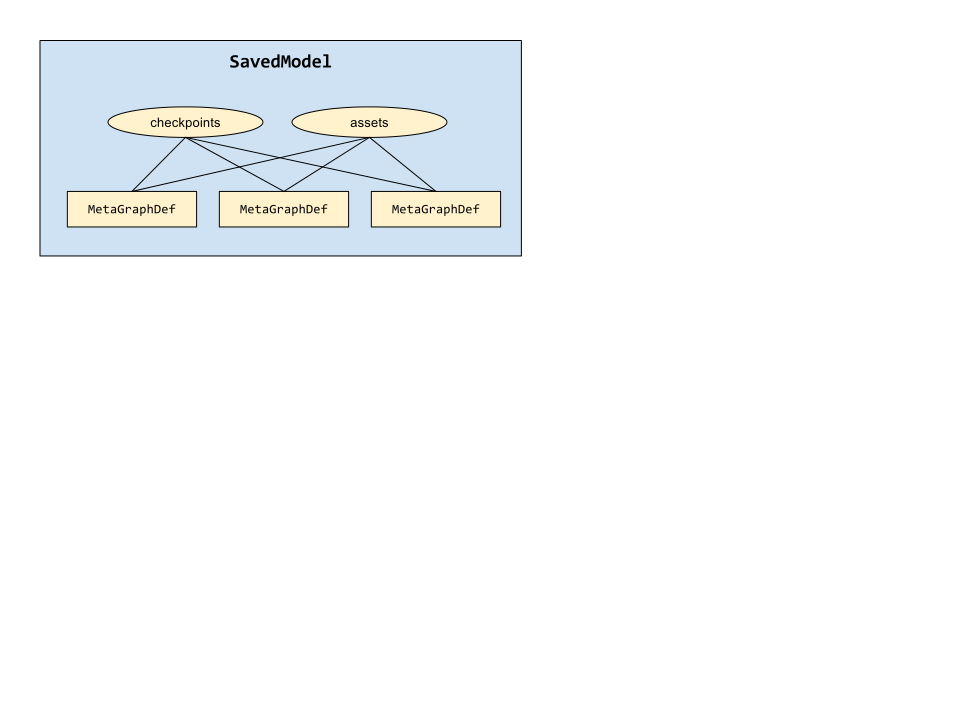
\includegraphics[width=\textwidth]{SavedModel.png}
\end{figure}
每张图介个指定的tags,使得在载入和恢复操作时确认可行。

\section{导入数据}
Dataset模块允许你从简单的,可重用的片段输入pipeline。例如图像模块的pipeline
也许集合分布式文件系统的数据,随机扰动每张图片,随机融合选中的图片为一个batch来训练,pipeline的text模型能利用元素提取的文本数据,转换它们为查找表embedding的标志符将不同长度的序列放在一起成为一个batch。Dataset API使得处理大型数据,不同数据格式和复杂的转换变得很容易。
一个 Dataset
 API包含两个TebsorFlow抽象。
\begin{itemize}
\item 一个tf.contrib.data.Dataset代表一个元素序列,其中的每个元素代表了一个或者更多的Tensor对象。例如在图像pipeline,一个元素可能是单个的训练样本(一对代表了label和图像数据的tensor)有两种方法创建数据集:
	\begin{enumerate}
		\item 创建一个源(Dataset.from\_tensor\_slices())从一个或者更多的tf.Tensor图像构造数据集。
		\item 应用转换格式从一个或者更多的tf.contrib.data.Dataset对象构造数据集。
	\end{enumerate}
	\item tf.contrib.data.Iterator提供主要的从数据集提取元素的方法当Iterator.get\_next()操作执行的时候从Dataset生成下一个元素,典型的行为作为输入pipeline和你的模型之间的接口。最简单的迭代器(iterator)是"one-shot iterator"它结合了数据集和迭代。用Iterator.initializer操作用不同的数据集重新初始化和参数化一个迭代器,例如在一个程序多次迭代训练样本和验证集。
\end{itemize}
\subsection{基本的机制}
为了开始一个输入pipeline你需要定义一个源。例如从内存中的一些tensor构造一个数据集。你可以使用tf.contrib.data.Dataset.from\_tensors()或者tf.contrib.data.Dataset.from
\newline \_tensor\_slices()。如果你的输入数据在磁盘上,推荐你用TFRecord
格式,你可以构造一个tf.contrib.data.TFRecordDataset。

当你有一个Dataset对象的时候,你可以通过链式方法调用tf.contrib.data.Dataset对象转化成新的Dataset。例如你可以用之前的元素转换作为Dataset.map()(应用一个函数到每个元素)多元素转换像Dataset.batch()。查看文档\href{https://www.tensorflow.org/api_docs/python/tf/contrib/data/Dataset}{tf.contrib.data.Dataset}完成列表转换。
最常用的方法是消耗从Dataset来的值创建一个迭代器对象,提供访问一个元素的数据集的元素一次(调用Dataset.make\_one\_shot\_iterator()),一个tf.contrib.data.Iterator提供两个操作:Iterator.initializer重新初始化你的迭代器状态;Iterator.get\_next()返回迭代器下一个元素的Tensor。
\subsection{数据结构}
一个数据集包含有相同结构的元素。一个元素包含一个或者更多称为组件的tf.Tensor对象。每个组件有tf.DType代表在tensor中元素的数据类型,Dataset.output\_types和Dataset.output\_shapes属性允许你查看每个数据集元素的组件的类型和形状。这些参数的嵌套结构映射元素的结构(也许是一个tensor,一个tensor元组,或者嵌套的tensor元组)
\begin{lstlisting}[language=Python]
dataset1 = tf.contrib.data.Dataset.from_tensor_slices(tf.random_uniform([4,10]))
print(dataset1.output_types)#tf.float32
print(dataset1.output_shapes)#(10,)
dataset2 = tf.contrib.data.Dataset.from_tensor_slices((tf.random_uniform([4]))
tf.random_uniform([4,100],maxval=100,dtype=tf.int32))
print(dataset2.output_types)#(tf.float32,tf.int32)
print(dataset2.output_shapes)#((),(100,))
datasets = tf.contrib.data.Dataset.zip((dataset1,dataset2))
print(dataset3.output_types)#(tf.float32,(tf.float32,tf.int32))
print(dataset3.output_shapes)#(10,((),(100,)))
\end{lstlisting}
给每个元素的组成命名是很方便的,例如它们代表不同训练样本的特征。另外,你可以用collections.namedtuple或者一个字典映射字符串到tensor代表Dataset的单个元素。
\begin{lstlisting}[language=Python]
dataset = tf.contrib.data.Dataset.from_tensor_slices({
	"a":tf.random_uniform([4]),
	"b":tf.random_uniform([4,100],maxval=100,dtype=tf.int32}))
print(dataset.output_types())#{'a':tf.float32,'b':tf.int32}
print(dataset.output_shape)#{'a':(),'b':(100,)}
\end{lstlisting}
Dataset转换支持任何的数据结构,当你用Dataset.map(),Dataset.flat\_map和Dataset.filter()转换应用函数到每个元素,元素结构决定函数的参数:
\begin{lstlisting}[language=Python]
dataset1 = dataset1.map(lambda x: ...)
dataset2 = dataset2.flat_map(lambda x, y: ...)
# Note: Argument destructuring is not available in Python 3.
dataset3 = dataset3.filter(lambda x, (y, z): ...)
\end{lstlisting}
\subsection{创建一个迭代器}
当你创建一个Dataset代表你的输入数据的时候,下一步是创建一个迭代器从数据集中访问元素,Dataset API当前支持一下迭代器:
\begin{itemize}
	\item one-shot
	\item initilizable
	\item reinitilizable
	\item feedable
\end{itemize}
one-shot迭代器是迭代器中最简单的形式,支持在数据集上迭代一次,不需要初始化。One-shot处理大多数的基于队列的输入pipeline,但是它们不支持参数化。用Dataset.range()作为例子:
\begin{lstlisting}[language=Python]
dataset = tf.contrib.data.Dataset.range(100)
iterator = dataset.make_one_shot_iterator()
next_element = iterator.get_next()
for i in range(10):
    value = sess.run(next_element)
    assert i == value
\end{lstlisting}
initializable迭代器要求你使用前明确的运行iterator.initializer操作。为此它允许你送入一个或者更多的tf.placeholder() tensor\textcolor{red}{初始化你的迭代器},继续用Dataset.range():
\begin{lstlisting}[language=Python]
#Base environ pass
max_value = tf.placeholder(tf.int64, shape=[])
dataset = tf.contrib.data.Dataset.range(max_value)
iterator = dataset.make_initializable_iterator()
next_element = iterator.get_next()
sess = tf.Session()
# Initialize an iterator over a dataset with 10 elements.
sess.run(iterator.initializer, feed_dict={max_value: 10})
for i in range(10):
    value = sess.run(next_element)
    assert i == value
# Initialize the same iterator over a dataset with 100 elements.
sess.run(iterator.initializer, feed_dict={max_value: 100})
for i in range(100):
    value = sess.run(next_element)
    assert i == value
\end{lstlisting}
一个reinitializable迭代器可以通过多个不同的Dataset对象初始化。例如你也许有一个用随机扰动输入图像提高泛化性的输入pipeline一个验证输入pipeline在没有修改的数据上评价预测。这些pipeline将用于相同结构(每个组件有相同的类型和兼容的形状)的不同的Dataset对象
\begin{lstlisting}[language=Python]
# Define training and validation datasets with the same structure.
training_dataset = tf.contrib.data.Dataset.range(100).map(
    lambda x: x + tf.random_uniform([], -10, 10, tf.int64))
validation_dataset = tf.contrib.data.Dataset.range(50)
# A reinitializable iterator is defined by its structure. We could use the
# `output_types` and `output_shapes` properties of either `training_dataset`
# or `validation_dataset` here, because they are compatible.
iterator = Iterator.from_structure(training_dataset.output_types,
training_dataset.output_shapes)
next_element = iterator.get_next()
training_init_op = iterator.make_initializer(training_dataset)
validation_init_op = iterator.make_initializer(validation_dataset)
# Run 20 epochs in which the training dataset is traversed, followed by the
# validation dataset.
for _ in range(20):
# Initialize an iterator over the training dataset.
    sess.run(training_init_op)
    for _ in range(100):
        sess.run(next_element)
    # Initialize an iterator over the validation dataset.
    sess.run(validation_init_op)
    for _ in range(50):
        sess.run(next_element)
\end{lstlisting}
一个feedable迭代器可以和tf.placeholder用在一起来调用tf.Session.run时选择什么通过deed\_dict机制。它提供相同的函数作为重新初始化迭代器,但是当你在不同数据集切换的时候不要求你从数据集开始初始化。例如用相同的训练验证样本你可以用tf.contrib.data.Iterator.from\_string\_handle定义一个feedable迭代器允许你在不同的数据集之间切换:
\begin{lstlisting}[language=Python]
# Define training and validation datasets with the same structure.
training_dataset = tf.contrib.data.Dataset.range(100).map(
    lambda x: x + tf.random_uniform([], -10, 10, tf.int64)).repeat()
validation_dataset = tf.contrib.data.Dataset.range(50)
# A feedable iterator is defined by a handle placeholder and its structure. We
# could use the `output_types` and `output_shapes` properties of either
# `training_dataset` or `validation_dataset` here, because they have
# identical structure.
handle = tf.placeholder(tf.string, shape=[])
iterator = tf.contrib.data.Iterator.from_string_handle(
        handle, training_dataset.output_types, training_dataset.output_shapes)
next_element = iterator.get_next()
# You can use feedable iterators with a variety of different kinds of iterator
# (such as one-shot and initializable iterators).
training_iterator = training_dataset.make_one_shot_iterator()
validation_iterator = validation_dataset.make_initializable_iterator()
# The `Iterator.string_handle()` method returns a tensor that can be evaluated
# and used to feed the `handle` placeholder.
training_handle = sess.run(training_iterator.string_handle())
validation_handle = sess.run(validation_iterator.string_handle())
# Loop forever, alternating between training and validation.
while True:
# Run 200 steps using the training dataset. Note that the training dataset is
# infinite, and we resume from where we left off in the previous `while` loop
# iteration.
    for _ in range(200):
        sess.run(next_element, feed_dict={handle: training_handle})
    # Run one pass over the validation dataset.
    sess.run(validation_iterator.initializer)
    for _ in range(50):
        sess.run(next_element, feed_dict={handle: validation_handle})
\end{lstlisting}
\subsection{消耗迭代器的值}
Iterator.get\_next()方法返回一个或多个迭代器的下一个元素tf.Tensor对象。每次迭代器被计算的时候它们得到数据集中的下一个元素,在TensorFlow中调用Iterator.get\_next()不会立即前进迭代器。相反你需要在一个TensorFlow表达式返回tf.Tensor对象,传递表达式的结果给tf.Session.run得到表达式的结果和下一个迭代器。
如果迭代器到大数据的尾部,执行Iterator.get\_next()操作将报出tf.errors.OutOfRangeError。这个点后迭代器将进入不稳定状态,你必须再次初始化它:
\begin{lstlisting}[language=Python]
dataset = tf.contrib.data.Dataset.range(5)
iterator = dataset.make_initializable_iterator()
next_element = iterator.get_next()
# Typically `result` will be the output of a model, or an optimizer's
# training operation.
result = tf.add(next_element, next_element)
sess.run(iterator.initializer)
print(sess.run(result))  # ==> "0"
print(sess.run(result))  # ==> "2"
print(sess.run(result))  # ==> "4"
print(sess.run(result))  # ==> "6"
print(sess.run(result))  # ==> "8"
try:
    sess.run(result)
except tf.errors.OutOfRangeError:
    print("End of dataset")  # ==> "End of dataset"
\end{lstlisting}
一个常用的模板是创建一个try-except块的训练循环包装器:
\begin{lstlisting}[language=Python]
sess.run(iterator.initializer)
while True:
    try:
        sess.run(result)
    except tf.errors.OutOfRangeError:
        break
\end{lstlisting}
如果数据集中的每个元素都有迭代的结构在相同的迭代结果下Iterator.get\_next()将返回一个或者更多的tf.Tensor。
\begin{lstlisting}[language=Python]
dataset1 = tf.contrib.data.Dataset.from_tensor_slices(tf.random_uniform([4, 10]))
dataset2 = tf.contrib.data.Dataset.from_tensor_slices((tf.random_uniform([4]), tf.random_uniform([4, 100])))
dataset3 = tf.contrib.data.Dataset.zip((dataset1, dataset2))
iterator = dataset3.make_initializable_iterator()
sess.run(iterator.initializer)
next1, (next2, next3) = iterator.get_next()
\end{lstlisting}
注意计算任何next1,next2或者next3将对所有的组件前进迭代器。一个典型的消耗迭代器将不能包含在单个表达式中的所有组件。
\subsection{读输入数据}
\subsubsection{消耗NumPy数据}
如果你的所有数据都适合于存储,一个简单的方法是用Dataset.from\_tensor\_slices()转换它们为tf.Tensor对象创建一个Dataset。
\begin{lstlisting}[language=Python]
# Load the training data into two NumPy arrays, for example using `np.load()`.
with np.load("/var/data/training_data.npy") as data:
    features = data["features"]
    labels = data["labels"]
# Assume that each row of `features` corresponds to the same row as `labels`.
assert features.shape[0] == labels.shape[0]
dataset = tf.contrib.data.Dataset.from_tensor_slices((features, labels))
\end{lstlisting}
注意上面的代码将在你的TensorFlow图中创建一个嵌入的features和labels作为一个tf.constant()操作。对于小的数据集这是很有用的,但是比较浪费存储,因为数据的内容将被多次复制可能达到tf.GraphDef protocal buffer的2GB限制。
\begin{lstlisting}[language=Python]
# Load the training data into two NumPy arrays, for example using `np.load()`.
with np.load("/var/data/training_data.npy") as data:
    features = data["features"]
    labels = data["labels"]
    # Assume that each row of `features` corresponds to the same row as `labels`.
assert features.shape[0] == labels.shape[0]
features_placeholder = tf.placeholder(features.dtype, features.shape)
labels_placeholder = tf.placeholder(labels.dtype, labels.shape)
dataset = tf.contrib.data.Dataset.from_tensor_slices((features_placeholder, labels_placeholder))
# [Other transformations on `dataset`...]
dataset = ...
iterator = dataset.make_initializable_iterator()
sess.run(iterator.initializer, feed_dict={features_placeholder: features,
                                        labels_placeholder: labels})
\end{lstlisting}
\subsection{消耗TFRecord数据}
一些数据集有一个或者多个文件。tf.contrib.data.TextLineDataset提供了一个简单的方法从一个或者更多text文件提取
行给定一个或者更多的文件名TextLineDataset将产生一个或者更多的字符串值元素。像TFRecordDataset,TextLineDataset接收filenames作为一个tf.Tensor,因此你可以通过tf.placeholder参数化它
\begin{lstlisting}[language=Python]
filenames = ["/var/data/file1.txt", "/var/data/file2.txt"]
dataset = tf.contrib.data.TextLineDataset(filenames)
\end{lstlisting}
默认情况下一个TextLineDataset产生文件的每一行,这也许并不是你想要的,例如一个文件的开头行有一些注释。这些行可以用Dataset.skip()移除和Dataset.filter()转换。为了在分割的文件应用这些转换,我们用Dataset.flat\_map()为每个文件创建一个迭代的Dataset
\lstinputlisting[language=Python]{./code/read_data.py}
\subsection{用Dataset.map()处理数据}
Dataset.map(f)通过使用函数f作用于输入数据集的每个元素生成一个新的数据集。它通过函数编程语言用map函数应用到列表。这个函数f接收tf.tensor对象代表一个单个的输入元素,返回一个代表一个数据集中单个元素tf.Tensor对象。它通过标准的TensorFlow操作转化一个元素为另一个。
\subsection{解析tf.Example protocal buffer消息}
一些输入的pipeline从TFRecord格式的文件提取tf.train.Example protocal buffer消息,用tf.python\_io.TFRecordWriter。每个tf.train.Example记录包含一个或者多个特征,输入pipline通常转换这些特征为tensor。
\begin{lstlisting}[language=Python]
# Transforms a scalar string `example_proto` into a pair of a scalar string and
# a scalar integer, representing an image and its label, respectively.
def _parse_function(example_proto):
    features = {"image": tf.FixedLenFeature((), tf.string, default_value=""),
                "label": tf.FixedLenFeature((), tf.int32, default_value=0)}
    parsed_features = tf.parse_single_example(example_proto, features)
    return parsed_features["image"], parsed_features["label"]

# Creates a dataset that reads all of the examples from two files, and extracts
# the image and label features.
filenames = ["/var/data/file1.tfrecord", "/var/data/file2.tfrecord"]
dataset = tf.contrib.data.TFRecordDataset(filenames)
dataset = dataset.map(_parse_function)
\end{lstlisting}
\subsection{解码图像数据变换大小}
当在一个真实世界的图像数据中训练一个神经网络,需要转换不同大小到一个同样的大小,因此它们也许处理为一个固定的尺寸
\begin{lstlisting}[language=Python]
# Reads an image from a file, decodes it into a dense tensor, and resizes it
# to a fixed shape.
def _parse_function(filename, label):
    image_string = tf.read_file(filename)
    #这里需要根据读取图片的数据编码格式,条用不同的解码函数
    image_decoded = tf.image.decode_png(image_string)
    image_resized = tf.image.resize_images(image_decoded, [28, 28])
    return image_resized, label

# A vector of filenames.
filenames = tf.constant(["/var/data/image1.jpg", "/var/data/image2.jpg", ...])

# `labels[i]` is the label for the image in filenames[i]
labels = tf.constant([0, 37, ...])
dataset = tf.contrib.data.Dataset.from_tensor_slices((filenames, labels))
dataset = dataset.map(_parse_function)
\end{lstlisting}
\subsection{用专门的Python logic}
考虑到性能要求,我们鼓励你尽可能用TensorFlow操作处理你的数据。然而当解析你的数据时有是有调用额外的python操作处理数据是有用的。为了这么做,在Dataset.map()转换中调用tf.py\_func()操作
\begin{lstlisting}[language=Python]
import cv2

# Use a custom OpenCV function to read the image, instead of the standard
# TensorFlow `tf.read_file()` operation.
def _read_py_function(filename, label):
  image_decoded = cv2.imread(image_string, cv2.IMREAD_GRAYSCALE)
  return image_decoded, label

# Use standard TensorFlow operations to resize the image to a fixed shape.
def _resize_function(image_decoded, label):
  image_decoded.set_shape([None, None, None])
  image_resized = tf.image.resize_images(image_decoded, [28, 28])
  return image_resized, label

filenames = ["/var/data/image1.jpg", "/var/data/image2.jpg", ...]
labels = [0, 37, 29, 1, ...]

dataset = tf.contrib.data.Dataset.from_tensor_slices((filenames, labels))
dataset = dataset.map(
    lambda filename, label: tf.py_func(
        _read_py_function, [filename, label], [tf.uint8, label.dtype]))
dataset = dataset.map(_resize_function)
\end{lstlisting}
\subsection{简单的批处理}
一个最简单的批处理是堆叠数据集中n个连续的元素。Dataset.batch()变换就是这么做的,和tf.stack()一样应用元素的每个组件,每个组件i所有的元素必须有一个相同的形状tensor。
\begin{lstlisting}[language=Python]
inc_dataset = tf.contrib.data.Dataset.range(100)
dec_dataset = tf.contrib.data.Dataset.range(0, -100, -1)
dataset = tf.contrib.data.Dataset.zip((inc_dataset, dec_dataset))
batched_dataset = dataset.batch(4)

iterator = batched_dataset.make_one_shot_iterator()
next_element = iterator.get_next()

print(sess.run(next_element))  # ==> ([0, 1, 2,   3],   [ 0, -1,  -2,  -3])
print(sess.run(next_element))  # ==> ([4, 5, 6,   7],   [-4, -5,  -6,  -7])
print(sess.run(next_element))  # ==> ([8, 9, 10, 11],   [-8, -9, -10, -11])
\end{lstlisting}
\subsection{批量的tensorpadding}
上面的方法要要求所有的元素有相同的尺寸,然而一些模型(sequence模型)中输入数据有不同的形状。为了处理这些情况,Dataset.padded\_batch()使你通过指定一个或者更多维(需要padding)转换不同形状的tensor为一个batch。
\begin{lstlisting}[language=Python]
dataset = tf.contrib.data.Dataset.range(100)
dataset = dataset.map(lambda x: tf.fill([tf.cast(x, tf.int32)], x))
dataset = dataset.padded_batch(4, padded_shapes=[None])

iterator = dataset.make_one_shot_iterator()
next_element = iterator.get_next()

print(sess.run(next_element))  # ==> [[0, 0, 0], [1, 0, 0], [2, 2, 0], [3, 3, 3]]
print(sess.run(next_element))  # ==> [[4, 4, 4, 4, 0, 0, 0],
                               #      [5, 5, 5, 5, 5, 0, 0],
                               #      [6, 6, 6, 6, 6, 6, 0],
                               #      [7, 7, 7, 7, 7, 7, 7]]
\end{lstlisting}
Dataset.padded\_batch()转换允许你为每组件的一维度设置不同的pading,它也许有变化的长度或者固定的长度,它可以覆盖padding的值(默认为0)。
\subsection{处理多epoch}
Dataset API提供了两个主要的方法处理相同数据的多个epochs,最简单的方法是用Dataset.repeat()变换数据集在多个epoch、例如,在输入中创建一个数据集10 epochs
\begin{lstlisting}[language=Python]
filenames = ["/var/data/file1.tfrecord", "/var/data/file2.tfrecord"]
dataset = tf.contrib.data.TFRecordDataset(filenames)
dataset = dataset.map(...)
dataset = dataset.repeat(10)
dataset = dataset.batch(32)
\end{lstlisting}
使用Dataset.repeat()变换没有参数重复输入将不确定。Dataset.repeat()变换连接它的参数每个epochs没有任何结束信号和下一个epoch的开始信号。如果你想接收每个epoch信号,你可以写一个循环在数据集的末尾捕获tf.errors.OutOgRange。
\begin{lstlisting}[language=Python]
filenames = ["/var/data/file1.tfrecord", "/var/data/file2.tfrecord"]
dataset = tf.contrib.data.TFRecordDataset(filenames)
dataset = dataset.map(...)
dataset = dataset.batch(32)
iterator = dataset.make_initializable_iterator()
next_element = iterator.get_next()

# Compute for 100 epochs.
for _ in range(100):
    sess.run(iterator.initializer)
    while True:
    try:
        sess.run(next_element)
    except tf.errors.OutOfRangeError:
        break

  # [Perform end-of-epoch calculations here.]
\end{lstlisting}
\subsection{随机打乱输入数据}
Dataset.shuffle()用和tf.RandomShuffleQueue方法随即打乱输入数据集,它保持一个固定的buffer平均的从bugger选择下一个元素(查看完整例子):
\begin{lstlisting}[language=Python]
filenames = ["/var/data/file1.tfrecord", "/var/data/file2.tfrecord"]
dataset = tf.contrib.data.TFRecordDataset(filenames)
dataset = dataset.map(...)
dataset = dataset.shuffle(buffer_size=10000)
dataset = dataset.batch(32)
dataset = dataset.repeat()
\end{lstlisting}
\subsection{用高级APIs}
tf.train.MonitoredTrainingSession API简化了一些在分布式方面运行方面的设置。MonidotedTrainingSession用tf.errors.outOfRangeError作为训练完成的标记,因此用Dataset API,我们推荐用Dataset.make\_one\_shot\_iterator()例如:
\begin{lstlisting}[language=Python]
filenames = ["/var/data/file1.tfrecord", "/var/data/file2.tfrecord"]
dataset = tf.contrib.data.TFRecordDataset(filenames)
dataset = dataset.map(...)
dataset = dataset.shuffle(buffer_size=10000)
dataset = dataset.batch(32)
dataset = dataset.repeat(num_epochs)
iterator = dataset.make_one_shot_iterator()

next_example, next_label = iterator.get_next()
loss = model_function(next_example, next_label)

training_op = tf.train.AdagradOptimizer(...).minimize(loss)

with tf.train.MonitoredTrainingSession(...) as sess:
    while not sess.should_stop():
        sess.run(training_op)
\end{lstlisting}
为了在tf.estimator.Estimator的input\_fn中使用一个Dataset,我们推荐用Dataset.make\_one\_shot\_iterator(),例如:
\begin{lstlisting}[language=Python]
def dataset_input_fn():
    filenames = ["/var/data/file1.tfrecord", "/var/data/file2.tfrecord"]
    dataset = tf.contrib.data.TFRecordDataset(filenames)

# Use `tf.parse\_single\_example()` to extract data from a `tf.Example`
# protocol buffer, and perform any additional per-record preprocessing.
    def parser(record):
        keys_to_features = {
            "image_data": tf.FixedLenFeature((), tf.string, default_value=""),
            "date_time": tf.FixedLenFeature((), tf.int64, default_value=""),
            "label": tf.FixedLenFeature((), tf.int64,
                                    default_value=tf.zeros([], dtype=tf.int64)),
    }
        parsed = tf.parse_single_example(record, keys_to_features)

        # Perform additional preprocessing on the parsed data.
        image = tf.decode_jpeg(parsed["image_data"])
        image = tf.reshape(image, [299, 299, 1])
        label = tf.cast(parsed["label"], tf.int32)

        return {"image_data": image, "date_time": parsed["date_time"]}, label

  # Use `Dataset.map()` to build a pair of a feature dictionary and a label 
  # tensor for each example.
  dataset = dataset.map(parser)
  dataset = dataset.shuffle(buffer_size=10000)
  dataset = dataset.batch(32)
  dataset = dataset.repeat(num_epochs)
  iterator = dataset.make_one_shot_iterator()

  # `features` is a dictionary in which each value is a batch of values for
  # that feature; `labels` is a batch of labels.
  features, labels = iterator.get_next()
  return features, labels
\end{lstlisting}
\section{线程和队列}
\begin{quote}
	\emph{注意在TensorFlow1.2之前我们推荐用多线程,队列输入pipeline,在TensorFlow1.2开始我们推荐使用tf.contrib.data模块。tf.contrib.data提供了一个更加简单的结构构建高效的输入pipeline,我们已经停止了之前正在开发的多线程和队列输入pipeline,我们帮依然维护旧的代码的开发者维护文档。}
\end{quote}
%多线程及时是一个强有力的而且广泛使用的支持一步计算的机制,入上面章节所述,TensorFlow计算图节点和计算图实现,一个队列是一个已经准备好的节点,向一个变量;以它节点可以修改它的内容。类似的,节点可以入队新的元素到队列或者从队列中出去已近存在的元素,TensorFlow队列提供了一个方法结合多个计算步。如果队列为空依然出队或者队列已满依然入队豆浆产生阻塞,挡这两个条件不满足的时候阻塞解除基础处理。TensorFlow实现了多个队列类,不同的类之间的不同是元素从队列移除的顺序。为了更好的理解我们考虑一个简单的情况我们创建"First in first out"队列然后填充0.然后我们构造一张图从队列中获取元素增加1,然后将它放在队列的尾部,慢慢地队列中的数字增加。
\begin{lstlisting}[language=Python]
sess = tf.Session()
q = tf.FIFOQueue(3,"float")
init = q.enqueue_many(([0.,0.,0.],))
x = q.dequeue()
y = x+1
q_inc = q.enqueue([y])
init.run(session=sess)
q_inc.run(session=sess)
q_inc.run(session=sess)
q_inc.run(session=sess)
q_inc.run(session=sess)
\end{lstlisting}
Enqueue,EnqueueMany和Dequeue是一个特别的节点。它们是指向队列真实值的指针,允许它们改变状态。我们推荐你考虑这些操作的时候用面向对象的理解,事实上在Python API中这些操作通过调用队列的方法。
\begin{quote}
	\emph{注意Queue方法必须运行在相同的设备上,不兼容的设备放置将在创建这些操作的时候被忽略}
\end{quote}
\subsection{队列用法}
像tf.FIFOQueue和tf.RandomShuffleQueue是在图上执行异步计算的重要的TensorFlow对象。典型的队列输入pipline用RandomShuffleQueue为训练模型准备输入:
\begin{itemize}
	\item 多线程准备训练数据和将数据入队
	\item 训练线程执行训练操作从队列出队mini-batch
\end{itemize}
我们推荐使用Dataset的shuffle和batch方法完成这个任务。然而,如果你仍然愿意使用队列版本,你可以在tf.train.shuffle\_batch中找到完美的实现。

下面展示一个简单的实现,这个函数获取一个source tensor,capacity和batch size作为参数返回一个批量打乱的出队tensor。
\begin{lstlisting}[language=Python]
def simple_shuffle_batch(source, capacity, batch_size=10):
  # Create a random shuffle queue.
    queue = tf.RandomShuffleQueue(capacity=capacity,
                                  min_after_dequeue=int(0.9*capacity),
                                  shapes=source.shape, dtypes=source.dtype)

    # Create an op to enqueue one item.
    enqueue = queue.enqueue(source)

    # Create a queue runner that, when started, will launch 4 threads applying
    # that enqueue op.
    num_threads = 4
    qr = tf.train.QueueRunner(queue, [enqueue] * num_threads)

    # Register the queue runner so it can be found and started by
    # `tf.train.start\_queue\_runners` later (the threads are not launched yet).
    tf.train.add_queue_runner(qr)

    # Create an op to dequeue a batch
    return queue.dequeue_many(batch_size)
\end{lstlisting}
当tf.train.start\_queue\_runners开始的时候,或者直接通过tf.train.MonitoredSession,QueueRunner将在后台开启进程填充队列,同时主线程执行dequeue\_many操作从中拉取数据,现在这些操作不相互依赖,除非间接地通过队列的内部依赖。简单的用这个函数像这样:
\begin{lstlisting}[language=Python]
# create a dataset that counts from 0 to 99
input = tf.constant(list(range(100)))
input = tf.contrib.data.Dataset.from_tensor_slices(input)
input = input.make_one_shot_iterator().get_next()

# Create a slightly shuffled batch from the sorted elements
get_batch = simple_shuffle_batch(input, capacity=20)

# `MonitoredSession` will start and manage the `QueueRunner` threads.
with tf.train.MonitoredSession() as sess:
    # Since the `QueueRunners` have been started, data is available in the
    # queue, so the `sess.run(get\_batch)` call will not hang.
    while not sess.should_stop():
        print(sess.run(get_batch))
\end{lstlisting}
输出
\begin{lstlisting}[language=Python]
[ 8 10  7  5  4 13 15 14 25  0]
[23 29 28 31 33 18 19 11 34 27]
[12 21 37 39 35 22 44 36 20 46]
\end{lstlisting}
对于更多的情况有tf.train.MonitoredSession提供的自动线程启动和管理是足够的,在极少的情况下不行,TensorFlow提供了手动管理你的线程的工具。
\subsection{手动线程管理}
正如我们看到的,TensorFlow Session是多线程的而且是线程安全的,因此多线程能够容易的在相同的会话和运行操作中使用。然而,不总是很容易实现一个Python程序按照要求驱动线程,所有的线程必须能同时停止,特别是必须捕获和报告,队列停止的时候必须被合适的关闭。TensorFlow提供了两个类:tf.train.Coordinator和tf.train.QueueRunner。这两个类帮助多线程一起停止,向程序报告异常等待它们停止,QueueRunner类被用于创建一个线程协作同一队列中的入队tensor。
\subsection{Coordinator}
tf.train.Coordinator类管理TensorFlow程序的后台线程帮助多线程一起停止,关键的方法是:
\begin{itemize}
	\item tf.train.Coordinator.should\_stop:如果线程应该被停止返回True。
	\item tf.train.Coordinator.request\_stop:请求应该停止的线程。
	\item tf.train.Coordinator.join:等待直到指定的线程被停止。
\end{itemize}
你首先创建一个Coordinator对象然后创建一些用于协调的线程。线程通常循环运行当shold\_stop为True是停止。任何线程都可以决定计算应该被停止。它仅仅必须调用request\_stop(),should\_stop()返回True是其它线程停止。
\begin{lstlisting}[language=Python]
# Using Python's threading library.
import threading

# Thread body: loop until the coordinator indicates a stop was requested.
# If some condition becomes true, ask the coordinator to stop.
def MyLoop(coord):
    while not coord.should_stop():
    ...do something...
    if ...some condition...:
        coord.request_stop()

# Main thread: create a coordinator.
coord = tf.train.Coordinator()

# Create 10 threads that run 'MyLoop()'
threads = [threading.Thread(target=MyLoop, args=(coord,)) for i in range(10)]

# Start the threads and wait for all of them to stop.
for t in threads:
  t.start()
coord.join(threads)
\end{lstlisting}
显然,coordinator可以管理线程做不同的事。它们不是必须和上面的例子一样。coordinator也支持捕获和报告异常,查看\href{https://www.tensorflow.org/api_docs/python/tf/train/Coordinator}{tf.train.Coordinator}文档查看更多信息。
\subsection{QueueRunner}
tf.train.QueueRunner类创建一些线程重复执行入队操作。这些线程可以用coordinator一起停止,另外一个队列runner将运行一个closer操作,如果在coordinator中的队列被报告异常将关闭队列。你可以用一个队列runner实现下面的架构,首先用一个TensorFlow为输入样本建立一个图,添加操作处理将样本送入队列,添加训练操作从队列出队。
\begin{lstlisting}[language=Python]
example = ...ops to create one example...
# Create a queue, and an op that enqueues examples one at a time in the queue.
queue = tf.RandomShuffleQueue(...)
enqueue_op = queue.enqueue(example)
# Create a training graph that starts by dequeueing a batch of examples.
inputs = queue.dequeue_many(batch_size)
train_op = ...use 'inputs' to build the training part of the graph...	
\end{lstlisting}
在Python的训练程序中,创建一个QueueRunner将运行一些线程处理入队样本、创建一个Coordinator要求queue runner用coordinator开启它的线程。用coordinator写一个训练循环。
\begin{lstlisting}[language=Python]
# Create a queue runner that will run 4 threads in parallel to enqueue
# examples.
qr = tf.train.QueueRunner(queue, [enqueue_op] * 4)

# Launch the graph.
sess = tf.Session()
# Create a coordinator, launch the queue runner threads.
coord = tf.train.Coordinator()
enqueue_threads = qr.create_threads(sess, coord=coord, start=True)
# Run the training loop, controlling termination with the coordinator.
for step in range(1000000):
    if coord.should_stop():
        break
    sess.run(train_op)
# When done, ask the threads to stop.
coord.request_stop()
# And wait for them to actually do it.
coord.join(enqueue_threads)
\end{lstlisting}
\subsection{处理异常}
线程通过队列runner启动做的比仅仅运行入队操作要多。它们捕获处理队列生成的异常,包括用于报告队列被关闭的tf.errors.OutOfRangeError异常。一个训练中的程序用一个coordinator必须类似的在主循环中捕获和报告异常。下面是上面训练循环的一个改进的例子:
\begin{lstlisting}[language=Python]
try:
    for step in range(1000000):
      if coord.should_stop():
        break
      sess.run(train_op)
except Exception, e:
    # Report exceptions to the coordinator.
    coord.request_stop(e)
finally:
    # Terminate as usual. It is safe to call `coord.request\_stop()` twice.
    coord.request_stop()
    coord.join(threads)
\end{lstlisting}
\section{embeddings}
一个embedding是一个从离散对象,像字映射为一个真实值的向量,例如一个英文字符的300维的embedding可能包括:
\begin{lstlisting}[language=Python]
blue:  (0.01359, 0.00075997, 0.24608, ..., -0.2524, 1.0048, 0.06259)
blues:  (0.01396, 0.11887, -0.48963, ..., 0.033483, -0.10007, 0.1158)
orange:  (-0.24776, -0.12359, 0.20986, ..., 0.079717, 0.23865, -0.014213)
oranges:  (-0.35609, 0.21854, 0.080944, ..., -0.35413, 0.38511, -0.070976)
\end{lstlisting}
embedding让你能在离散的数据上应用机器学习,分类器,更常用的神经网络都被设计为一个高密度的连续向量(所有的值都用来定义一个对象)如果离散对象被编码为一个离散的原子,有独一无二的id号,它们阻止学习和泛化,一种考虑embeddings的方法是转化非向量的对象为有用的机器学习输入。,embeding作为机器学习的输出也是有用的,因为embedding映射对象为向量,在向量空间中的应用是类似的。一个通常的用法是找到一个最接近的邻居。用和相面相同的word embedding,例如对于每个字和相关的角度这里有三个接近的邻居:
\begin{lstlisting}[language=Python]
blue:  (red, 47.6°), (yellow, 51.9°), (purple, 52.4°)
blues:  (jazz, 53.3°), (folk, 59.1°), (bluegrass, 60.6°)
orange:  (yellow, 53.5°), (colored, 58.0°), (bright, 59.9°)
oranges:  (apples, 45.3°), (lemons, 48.3°), (mangoes, 50.4°)
\end{lstlisting}
这将告诉程序苹果和橙子类似度($45.3^o$)比柠檬和橙子($48.3^o$)更类似。
\subsection{训练一个embedding}
为了在TensorFlow中训练word embedding,首先你需要分隔文字成单词赋值给词汇表中的每一个单词一个整数。假设我们已经做了这步,word\_ids是一个整数向量。例如句子"I have a cat."可能被分割成["I","have","a","cat","."]然后相关的word\_ids tensor形状为[5]由5个整数组成。为了得到这些单词ids embeded,我们需要用tf.gather函数按照下面创建embedding变量。
\begin{lstlisting}[language=Python]
word_embeddings = tf.get_variable(“word_embeddings”,
    [vocabulary_size, embedding_size])
embedded_word_ids = tf.gather(word_embeddings, word_ids)
\end{lstlisting}
在这之后tensor embedded\_word\_ids在我们的例子中将有形状[5,embedding\_size]同时包含5个单词的embeddings(dense vector)。变量word\_embeddings将被学习,在训练结束后它将包含所有在词汇表中的embeddings。embeddings可能被多种方式训练,依靠数据变量。例如可以用循环神经网络从语料中的句子的前一个单词预测下一个单词或者用两个网络做多种语言的翻译。这个方法在\textbf{字词的向量表示}中有描述,但是上面的所有情况下有一个像上面的embedding变量和用tf.gather的embbedded word。
\subsection{可视化Embeddings}
TensorBoard有一个内建的可视化器,称为EmbeddingProjector,用于交互式的embedding可视化。embedding projector将从你的checkpointer文件读取embeddings用PCA映射它们到3维空间。对于PCA的可视化查看\href{http://setosa.io/ev/principal-component-analysis/}{这里},另一个有用的映射是t-SNE。如果你正在embedding上工作,你可能像添加labels/images到数据点。你可以通过生成一个包含每个点的labels和用我们的Python API映射器的配置\href{https://www.tensorflow.org/programmers_guide/embedding#metadata}{metadata file},或者在和你的checkpoint文件相同多个目录手动构造和保存一个projector\_config.pbtxt。
\subsection{创建}
\begin{enumerate}
	\item 设置一个2维tensor保存你的embedding。
		\begin{lstlisting}[language=Python]
			embedding_var = tf.get_variable(...)
		\end{lstlisting}
	\item 定期保存你模型的变量到LOG\_DIR目录中
		\begin{lstlisting}[language=Python]
			saver = tf.train.Saver()
			saver.save(session,os.path.join(LOG_DIR,"model.ckpt"),step)
		\end{lstlisting}
	\item 结合meta data和你的embedding(可选)
\end{enumerate}
如果你有任何的metadata(labels,images)结合你的embedding,你可以调用TensorBoard通过指定存储在LOG\_DIR中的一个projector\_config.pbtxt或者用你自己的PythonAPI。例如下面的projector\_config.pbtxt结合word\_embedding tensor和存储在\$LOG\_DIR/metadata.tsv的metadata文件。
\begin{lstlisting}[language=Python]
embeddings {
	  tensor_name: 'word_embedding'
	    metadata_path: '$LOG_DIR/metadata.tsv'
	   }
\end{lstlisting}
相同的配置可以通过下面的代码段一程序产生:
\begin{lstlisting}[language=Python]
from tensorflow.contrib.tensorboard.plugins import projector
# Create randomly initialized embedding weights which will be trained.
vocabulary_size = 10000
embedding_size = 200
embedding_var = tf.get_variable('word_embedding', [vocabulary_size, embedding_size])
# Format: tensorflow/tensorboard/plugins/projector/projector_config.proto
config = projector.ProjectorConfig()
# You can add multiple embeddings. Here we add only one.
embedding = config.embeddings.add()
embedding.tensor_name = embedding_var.name
# Link this tensor to its metadata file (e.g. labels).
embedding.metadata_path = os.path.join(LOG_DIR, 'metadata.tsv')
# Use the same LOG_DIR where you stored your checkpoint.
summary_writer = tf.summary.FileWriter(LOG_DIR)
# The next line writes a projector_config.pbtxt in the LOG_DIR. TensorBoard will
# read this file during startup.
projector.visualize_embeddings(summary_writer, config)
\end{lstlisting}
在你运行你的模型和训练你的embedding后,运行TensorBoard和指定job的LOG\_DIR
\begin{lstlisting}[language=Python]
tensorboard --logdir=LOG_DIR
\end{lstlisting}
点击顶端面板的Embedding选择合适的运行。
\subsection{metdadata}
通常embeddings有metedata结合。metadata应该被存储在和模型的checkpoint分隔的文件中,因此metadata不是可训练的模型的参数。这是应该为\href{https://en.wikipedia.org/wiki/Tab-separated_values}{TSV file}(显示红色标签),第一行十粗体显示的表头和包含metadata值得子序列行。
\begin{lstlisting}{language=Python}
Word\tFrequency
Airplane\t345
Car\t241
...
\end{lstlisting}
有不明确的和主要数据文件的关键共享,而不是在madatada文件中的顺序和embedding tensor里面的顺序相匹配,换句话说第一行是头信息,metadata文件中(i+1)行和存储在checkpoint文件中的embedding tensor的第i行相关。
\begin{quote}
	\emph{如果TSV metadata文件仅仅有一列,我们不需要第一行假设每一行是embedding的label,我们包括这个例外,因为它匹配通常用的"vocab file"格式。}
\end{quote}
\subsection{图像}
如果你有图像和你的embedding结合,你将需要生成一个每个数据点缩略图组成的图像。它被称为\href{https://www.google.com/webhp#q=what+is+a+sprite+image}{sprite image}。sprite应该有和存储进行优先顺序的缩略图相同的行和列:第一个数据点放在是左上角最后一个数据放在右下角。

\begin{tabular}{|c|c|c|}
	\hline
	0&1&2\\
	\hline
	3&4&5\\
	\hline
	6&7&\\
	\hline
\end{tabular}

注意上面例子的最后一个元素不是必须填,对于具体的sprite例子查看10000张手写体数据\href{https://www.tensorflow.org/images/mnist_10k_sprite.png}{sprite image}
\begin{quote}
	\emph{注意我们当前支持$8192px\times8192px$}
\end{quote}
在够早了sprite后你需要告诉Embedding Projector到哪里寻找它:
\begin{lstlisting}[language=Python]
embedding.sprite.image_path = PATH_TO_SPRITE_IMAGE
	# Specify the width and height of a single thumbnail.
	embedding.sprite.single_image_dim.extend([w, h])
\end{lstlisting}
\subsection{交互}
Embedding Projector有三个面板:
\begin{enumerate}
	\item 左上角的Data面板,你也已选择运行embedding tensor和数据列标上颜色和label points。
	\item 左下角的Projections面板选择projection的类型(PCA,tSNE)
	\item 右边的Insepctor面板,这里你能搜索类似的点查看最近邻居的列表
\end{enumerate}
\subsection{Projections}
Embedding Projector有三种方法减少数据集的维度:两个线性一个非线性。每二个方法可以被用来创建一个二维或者三维视图。

PCA:一个直接的降维技术,Embedding projectorj计算10个主成分。菜单让你映射这些成分为任何二维或者三维。PCA是一个线性projection,检查全局结构时很有效
。

t-SNE:一个流行的非线性降维Embedding Projector提供二维和三维视图。客户端执行算法的每一步都被更新动画。因为t-SNE经常保留一些本地结构,对于本利邻居和发现集群是很有用的。尽管对于高维数据可视化很有用,t-SNE画图可能会有一些神秘或者难以理解,查看\href{http://distill.pub/2016/misread-tsne/}{great artical}查看t-SNE如何高效使用。

Custom:你也可以构造基于文本搜索查找在空间中有用的方向的特别的线性projections。为了定义一个projection轴,输入两个搜索字符串或者正则表达式。程序计算标签和搜索结果配的标签的中心,在不同的向量中心作为一个projection轴。
\subsection{导航}
为了探索数据集,用2维或者3维视图查看,缩放,旋转和用自然的手势点击和拖动面板。点击一个点引起右边面板显示一个确定的最相邻的文本列表。最相邻的点本身在projection被强调。

缩放进入集群给定一些信息,但是有时候更有用的是限制自己点的视角和在这些点上执行projection。,你可以用多种方式选择点:
\begin{enumerate}
	\item 在点击点后,相邻的点也被选中。
	\item 在搜索后匹配的查询被选中。
	\item Embedding选择,点击一个点拖动定义一个选择范围。
\end{enumerate}
在选择一个数据集点后,你可以用右边的inspector面板隔离这些点用isolate Pointes进一步分析,
\begin{figure}[H]
	\includegraphics[width=\textwidth]{embedding-nearest-points.png}
	\caption{important最相邻的embedding数据集}
\end{figure}
custom projection结合过滤会很有用,下面我们过滤和"politics"100个最相邻的点,project它们在x轴上从好到坏,向量表示,y轴水机。你可以看右边的我们有"ideas","science",\newline "perspective","journalism"左边有"crisis","violence"和"conflict"。
\begin{figure}
\includegraphics[width=\textwidth]{embedding-custom-projection.png}
\end{figure}

\subsection{合作的特性}
为了分享你的发现你可以用右上角的bookmark面板保存当前状态(包括计算任何projection的坐标)为一个小文件。Projector可能被指定到一个或者更多文件,产生下面的面板,其它人可以通过标签序列查看。
\begin{figure}[H]
	\includegraphics[width=\textwidth]{embedding-bookmark.png}
\end{figure}
\subsection{简单的问答}
embedding是一个动作还是一个事物?两者都是,人们谈论向量空间的embedding word形成embedding(事物)。通常两个是一个从离散对象到向量映射embedding概念,创建应用映射是一个行为,但是映射是一个事物。

是高维还是低维embedding?300维的向量字词空间,例如当和上百万的字词空间相比是低维。但是数学上它是高维,显示了大量和人们直觉上的2维或者三维空间不一致的特性。

embedding和embedding layer是一样的吗?不是,一个embedding layer是神经网络的一部分,不是一个embedding是一个更常用的概念。
